\documentclass[openright, twoside, british]{book}

\usepackage[utf8]{inputenc}
\usepackage{kotex}
\usepackage{ptmt}

\title{Fundamentals of Problem Solving}
\author{Mingeon Jeong \and Donghyun Gu}
\date{\today}

\begin{document}

% Front matter section.
\frontmatter

% Include the title page, which is located in the FrontMatter subfolder.
\include{./FrontMatter/titlepage}

% Create the book's title page.
\maketitle\pagebreak

\tableofcontents

\mainmatter

\part{서론}
\chapter{시간 복잡도와 공간 복잡도}
\section{개요}
\label{sec: start}
Problem Solving에 필요한 알고리즘 공부에 앞서, 알고리즘을 평가하는 방법을 알 필요가 있다. 보통 알고리즘의 평가는 \textbf{시간과 메모리}의 두 가지 측면에서 이루어진다. Problem Solving에서 시간 제한과 메모리 제한은 문제를 풀기 전에 꼭 확인해야 하는 요소 중 하나이며, 시간 제한에 따라 문제 풀이가 달라지기도 한다.

당연하게도 시간과 메모리는 제약 조건(Constraint)에 대한 함수로 표시될 것이다. 아주 간단히 1부터 $n$까지 수의 합을 구하는 문제와 이에 대한 아래 두 가지 알고리즘을 보자:

\begin{itemize}
    \item 알고리즘 1: 반복문을 이용해 $1$부터 $n$까지 순서대로 구한다.
    \item 알고리즘 2: $\sum_{i=1}^n i = \frac{n(n+1)}{2}$ 공식을 이용해 구한다.
\end{itemize}

직관적으로 알고리즘 1보다 알고리즘 2가 더 빠른 시간에 작동할 것이라고 추측할 수 있고, 실제로 그렇다(궁금한 사람은 $n=100,000,000$ 정도를 대입하여 직접 실행해보자). 그렇다면 정학히 얼마나 더 빠를까?

이에 대한 답을 명확히 줄 수 있는 수학적 기호가 바로 시간 복잡도와 공간 복잡도이다. 알고리즘 1의 시간 복잡도와 공간 복잡도를 보면 반복문에서 $n$번의 연산을 하고, 답에 저장하는 변수 하나만 필요하므로 메모리는 $1$이 필요하다고 생각할 수 있다. 반면 알고리즘 2의 경우에는 반복문 없이 총 세 번의 연산으로 답을 구할 수 있다. 이 알고리즘의 경우에는 시간 복잡도는 $3$로 줄어들고 공간 복잡도는 여전히 $1$이다. 즉, 알고리즘 2가 알고리즘 1보다 $n$배 빠르다고 말할 수 있다.

이런 의문이 들었을 수도 있다: 정확히는 $n/3$배 빠른 것 아닌가? 위에서 $n$으로 표시한 이유는 시간 복잡도와 공간 복잡도에서 상수가 크게 중요하지 않기 때문이다. 시간 복잡도와 공간 복잡도는 정확히 얼마의 시간이 걸리는지 알기 위한 것이 아니라, 제약조건에 따라 어느 정도로 시간이 빠르게 증가하는지를 확인하고자 하는 것이다. 즉, 우리는 시간에 가장 큰 영향을 주는 항만 남겨 표기해야 한다. 그리고 이를 수학적으로 나타내기 위해 점근 표기법(asymptotic notation)을 사용한다.

\section{점근 표기법}
점근 표기법이란, 함수가 증가 또는 감소하는 경향성을 나타내기 위한 표기법이다. 대표적으로는 Big-O, small-o, Big-Theta, small-theta, Big-Omega, small-omega 표기법이 있으며, 이 중 이 책에서는 PS에서 자주 쓰이는 Big-O와 Big-Theta notation에 대해서만 서술할 것이다. 이들의 정의는 다음과 같다.
\begin{definition}[Big-O notation]
    $\limsup_{x\to\infty} f(x)/g(x)<\infty$이면 $f(x)=O(g(x))$이다.
\end{definition}
\begin{definition}[Big-Theta notation]\label{def: big-theta}
    $\limsup_{x\to\infty} f(x)/g(x)<\infty$이고 $\liminf_{x\to\infty} f(x)/g(x)$ $>0$이면 $f(x)=\Theta(g(x))$이다.
\end{definition}
위 정의에서 보다시피 Big-O notation은 $f(x)$의 점근적 상한, Big-Theta notation은 $f(x)$의 점근적 상한이자 하한을 나타내는 것으로, Big-Theta가 더 엄밀한 값을 나타낸다는 것을 알 수 있다. 하지만 PS에서는 이 둘을 혼용해서 모두 \Cref{def: big-theta}의 정의로 사용하며, 이 책에서도 이후로 나오는 Big-O notation에 대한 정의는 예의 정의로 쓰일 것이다.

이제 시간 복잡도를 표기하는 방법을 알아보기 위해 앞의 예시를 다시 한 번 가져와보자.
\begin{itemize}
    \item 알고리즘 1: 반복문을 이용해 $1$부터 $n$까지 순서대로 구한다.
    \item 알고리즘 2: $\sum_{i=1}^n i = \frac{n(n+1)}{2}$ 공식을 이용해 구한다.
\end{itemize}
\cref{sec: start}에서 분석한 내용과 같이 알고리즘 1에는 $n$번의 연산이 쓰이며, 알고리즘 2에는 3번의 연산이 쓰인다. 이를 Big-O notation으로 표현한다면 알고리즘 1은 $O(n)$의 시간 복잡도를, 알고리즘 2는 $O(1)$의 시간 복잡도를 가진다고 표현할 수 있다(\Cref{def: big-theta}에서는 계수가 포함되어도 상관이 없지만, 이제부터는 그 상수를 생략하고 표기할 것이다).

공간 복잡도에 대해서도 같은 표기법을 사용한다는 것을 알아두자.

\section{제한 시간과 시간 복잡도}
현재 컴퓨터는 1초에 약 $10^8$번 정도, 많게는 $10^9$번 정도의 연산을 수행할 수 있다고 알려져 있다. PS 문제를 푼다면 본인이 생각한 풀이의 시간 복잡도를 분석하여 그 식에 입력 제한을 대입하여 제한 시간 안에 풀이가 답을 찾을지 확인하는 것이 좋다. 다음은 PS에서 사용되는 대표적인 시간 복잡도이다.
\begin{itemize}
    \item 상수 시간 복잡도, $O(1)$
    \item 로그 시간 복잡도, $O(\log N), O(\log^2 N)$ 등
    \item 루트 시간 복잡도, $O(\sqrt N)$
    \item 다항 시간 복잡도, $O(N), O(N^2)$ 등
    \item 지수 시간 복잡도, $O(2^N), O(3^N)$ 등
    \item 팩토리얼 시간 복잡도, $O(N!)$
\end{itemize}
보통 시간 복잡도는 위 예시들의 합 또는 곱으로 이루어진다.

\section{연습문제}
\begin{problem}
    크기 $N$의 어떤 집합 $S$의 모든 부분집합을 출력하려고 한다. 완전 탐색 방식의 시간복잡도는 무엇인가?
\end{problem}
\begin{problem}
    $N$개의 노드로 이루어진 완전 이진 트리의 리프에서 루트까지 올라가는 경로를 출력하고자 한다. 시간복잡도는 무엇인가?
\end{problem}

(추가될 예정)

\part{기본 알고리즘}
\chapter{백트래킹}
백트래킹(backtracking)은 해를 찾는 도중 해가 아니어서 막히면, 되돌아가서 다시 해를 찾아가는 알고리즘으로 최적화 문제와 결정 문제를 푸는데 쓰이며, 구현 시 재귀함수를 사용한다. 대표적인 문제들로 재귀함수의 사용법과 백트래킹을 익혀보자.

\section{이론}
스도쿠와 같은 퍼즐을 컴퓨터로 어떻게 풀 수 있을까? 가장 쉬운 방법은 모든 방법을 시도하는 것이다. 이를 위해 경우의 수를 셀 때 썼던 수형도(나뭇가지 그림)과 같은 아이디어를 쓸 수 있다. 첫 번째 칸에서 1~9 중 하나를 시도하고, 그 다음 칸에서 또 1~9중 하나를 시도하고, 이를 반복하는 완전 탐색을 하는 것이다. 빈 칸이 $t$개인 스도쿠를 푼다면, 총 $9^t$개의 경우를 시도하게 될 것이다.

하지만 꼭 모든 경우를 탐색해야 할까? 스도쿠에서 처음 두 칸에 모두 1을 채우는 것은, 뒤에 칸이 어떻게 채워지던지 불가능하다. 즉, 탐색을 하다가 중간에 불가능하다는 결론이 나오면 그 이후는 시도할 필요가 없다! 이 경우에는 다시 되돌아가서 다른 경우를 시도할 수 있다. 이처럼, 완전 탐색을 하되, 자명하게 불가능한 경우를 제외하여 시간의 효율을 조금 더 향상시킨 것이 백트래킹이다.

즉, 문제가 상수 개 중 하나를 선택하는 것을 여러 번 반복한다면, 백트래킹을 고려할 수 있다. 이때, 어느 순서로 채우는지에 따라 소요되는 시간이 크게 영향받을 수 있으므로, 좋은 방식을 찾는 것이 중요하다. 이제, 몇 가지의 예시 문제들로 백트래킹을 익히자.

\section{$N$-Queen 문제}
다음과 같은 문제를 생각해보자.
\begin{example}[$N$-Queen problem]\label{ex: n-queen}
    $N \times N$ 체스판 위에 $N$개의 퀸을 놓고자 한다. 가능한 경우가 존재하면 가능한 경우 한 가지를 출력하고, 그렇지 않으면 $-1$을 출력하라. 단, $N \leq 25$이다.
\end{example}
효율적 구현을 위해서는 어떤 순서로 선택을 할 지 결정해야 한다. 다음 관찰이 도움을 준다.

\begin{obs}
    한 가로줄에는 최대 하나의 퀸만 위치할 수 있다. 따라서 $N$개의 퀸을 놓으려면 정확히 하나의 가로줄에 하나의 퀸이 위치해야 한다.
\end{obs}

즉, 각 가로줄마다 하나의 퀸이 어디 위치할 지 $N$개 중에 하나를 선택하는 문제로 바꿀 수 있다. 이렇게 제일 위 가로줄부터 채우는 방식을 쓰기 위해 재귀함수 \texttt{solve}의 파라미터로 현재까지 퀸의 위치를 정한 가로줄의 개수 $L$을 사용할 것이다. 당연히 $L$은 현재까지 놓은 퀸의 개수와 같다. 그러면 \texttt{solve(L)}은 $L+1$번째 가로줄에 있는 $N$개의 칸에 퀸이 놓일 수 있는지 시험해 가능한 경우에 대해 모두 \texttt{solve(L+1)}을 호출하는 것으로 문제를 해결할 수 있다. 이 과정을 반복해 $L=N$에 도달하면 $N$개의 퀸을 놓았다는 뜻이므로, 현재 퀸의 위치를 출력하고 코드를 종료하면 된다. 만약 모든 경우를 시험했음에도 불구하고 코드가 종료되지 않았다면, 불가능하다는 뜻이므로 $-1$을 출력하고 코드를 종료하면 된다.

그렇다면 어떤 칸에 퀸이 놓일 수 있는지 어떻게 판단할 수 있을까? 그 퀸이 있는 세로줄, 가로줄, 그리고 두 방향에 대각선들에 있는 칸에 대해 다른 퀸이 있는지 확인하면 된다. 한 가로줄에 퀸 하나임은 보장되므로 가로줄은 확인할 필요가 없고, 아래쪽에 퀸이 없음이 보장되므로 위쪽에 있는 가로줄만 확인하면 된다. 이 과정은 정답 코드의 \texttt{isvaild(r, c)} 함수에서 처리된다.

\begin{code} \label{code: n-queen}
\Cref{ex: n-queen}의 정답 코드
\begin{lstlisting}
#include <bits/stdc++.h>
using namespace std;

int n, board[25][25];

bool isvaild(int r, int c) {
    for (int i = 0; i < r; i++) {
        if (board[i][c] == 1) return false;
    }

    int k = 1;
    while (true) {
        if (r + k >= n || c - k < 0) break;
        if (board[r + k][c - k] == 1) return false;
        k++;
    }
    k = 1;
    while (true) {
        if (r - k < 0 || c - k < 0) break;
        if (board[r - k][c - k] == 1) return false;
        k++;
    }

    return true;
}

void solve(int L) {
    if (L == n) {
        for (int i = 0; i < n; i++) {
            for (int j = 0; j < n; j++) cout << board[i][j] << " ";
            cout << "\n";
        }
        exit(0);
    }
    for (int i = 0; i < n; i++) {
        if (isvaild(L, i)) {
            board[L][i] = 1;
            solve(L + 1);
            board[L][i] = 0;
        }
    }
}

int main() {
    cin >> n;
    solve(0);
    cout << "-1\n";
    return 0;
}
\end{lstlisting}

\end{code}

\section{순열 구하기}

다음으로 백트래킹으로 주어진 조건을 만족하는 수열을 구하자. 고등학교 확률과 통계에서 배우는 것과 비슷한 느낌의 문제다.

\begin{example} $1 \leq M \leq N \leq 8$을 만족하는 두 정수 $N$과 $M$이 주어질 때, 각 조건을 만족하는 길이가 $M$인 \textbf{서로 다른 수열을 사전 순으로 모두} 출력하는 프로그램을 작성하라.
    \begin{itemize}
        \item (15649번) $1$부터 $N$까지 자연수 중에서 중복 없이 $M$개를 고른 수열
        \item (15650번) $1$부터 $N$까지 자연수 중에서 중복 없이 $M$개를 고른 \textbf{단조증가} 수열
        \item (15651번) $1$부터 $N$까지 자연수 중에서 \textbf{중복이 가능하게} $M$개를 고른 수열
        \item (15652번) $1$부터 $N$까지 자연수 중에서 \textbf{중복이 가능하게} $M$개를 고른 \textbf{단조증가} 수열
    \end{itemize}
\end{example}

이 문제에서도 \Cref{code: n-queen}에서 $L$에 대응하는 것을 잡아야 한다. 첫 번째 수부터 차례로 고르는 것이 제일 편하다. 따라서 현재까지 고른 수의 개수를 $L$로 두고 구현한다. 또한, 이 문제에서는 수열을 출력해야 하므로 지금까지 선택한 것을 저장해야 한다. 동적 자료구조인 \texttt{std::vector}을 아래와 같이 활용하면 편하다.

\begin{lstlisting}
#include <vector>
using namespace std;

vector<int> path;
void solve(int L) {
// ...
    path.push_back(i);
    solve(L+1);
    path.pop_back();
// ...
}
\end{lstlisting}

책에서는 이러한 방식을 재귀함수의 경로 기록이라고 할 것이다. 책에서 \texttt{path}라는 벡터 변수가 사용된다면, 함수 호출에 따른 경로를 기록한 경우가 많을 것이다.

이제 직접 네 문제를 구현해보라. 조건이 약간씩 다르기 때문에 세부적인 코드는 조금씩 변경해야 할 것이다. 이후의 과정은 독자에게 맡긴다.

이제, 비슷하지만 조금 더 어려운 문제를 보자.

\begin{example} $1 \leq M \leq N \leq 8$을 만족하는 두 정수 $N$과 $M$, 그리고 $N$개의 수로 이루어진 수열 $A_i$가 주어질 때, 각 조건을 만족하는 길이가 $M$인 \textbf{서로 다른 수열을 사전 순으로 모두} 출력하는 프로그램을 작성하라. 단, $N$개의 주어지는 수들 중에는 \textbf{같은 수가 있을 수 있다}.
    \begin{itemize}
        \item (15663번) 수열 $A_i$에서 중복 없이 $M$개를 고른 수열
        \item (15664번) 수열 $A_i$에서 중복 없이 $M$개를 고른 \textbf{단조증가} 수열
        \item (15665번) 수열 $A_i$에서 \textbf{중복이 가능하게} $M$개를 고른 수열
        \item (15666번) 수열 $A_i$에서 \textbf{중복이 가능하게} $M$개를 고른 \textbf{단조증가} 수열
    \end{itemize}
\end{example}

이 문제의 차이점은 $N$개의 수 중에 같은 수가 있을 수 있다는 것이다. 같은 수가 있으면, 이전 문제와 같은 방식으로 구현한 코드에서 출력하는 수열이 모두 다르다는 보장을 할 수 없다. 즉, 어떤 경우에 같아지는지 생각하고, 그 경우를 배제해야 한다. 같아지는 경우는 배열에 똑같은 수가 $a$번째와 $b$번째에 있을 때, 선택된 위치 중에서 $a$만을 $b$로 바꾼 경우이다. 즉, 아무것도 선택되지 않거나, $a$만 선택되거나, $a$와 $b$가 모두 선택되는 경우만 남기면 된다. 이것은 똑같은 수 중에서 더 앞에 있는 수가 선택되지 않았으면, 그 수를 선택하지 않는 방법으로 해결할 수 있다.

판단이 어렵다고 생각할 수 있지만, 배열을 처음에 정렬하고 시작함을 상기하자. 정렬된 배열에서 똑같은 수는 항상 연속된 위치에 있다. 이를 이용하면 구현을 쉽게 할 수 있다. 이후의 과정은 독자에게 맡긴다.

\section{격자 이동}
백트래킹을 사용하면 길을 찾을 수도 있다. 격자에서 상하좌우로만 이동할 수 있다면, 이것 자체도 4개 중에 하나를 선택하는 것을 반복하는 것이기 때문이다. 이와 관련된 문제를 하나 보자.

\begin{example} \label{ex: boj-1502}
    (1502번) $n \times m$ 격자에 두 개의 1이 적혀 있다. 두 개의 1 사이를 상하좌우로 인접한 칸으로 선을 그어 이으려고 한다. 선이 모든 칸을 다 지나야 할 때 가능한 이동 경로를 지나는 칸의 좌표로 출력하는 프로그램을 작성하라. 만약 가능한 경우가 없다면 \texttt{-1}을 출력한다. $m$과 $n$은 $2$ 이상 $8$ 이하의 짝수이다.
\end{example}

이 문제에서도 $L$에 대응하는 것을 생각하자. 지금까지 지난 칸의 수를 $L$로 잡으면 편하게 구현할 수 있을 것이다. 물론, 현재 칸에 따라 다음 칸이 달라지기 때문에 현재 칸의 위치를 나타내는 좌표도 파라미터로 넣어야 한다.

이 문제에 유용한 테크닉이 하나 있다. 격자에서 상하좌우로 이동하는 것은 현재 위치에서 $(-1, 0), (1, 0), (0, -1), (0, 1)$ 중 하나를 더하는 것과 같은데, 이것을 직접 작성해서 처리해도 되지만, 아래 코드와 같이 배열을 활용하면 조금 더 간단하게 할 수 있다.

\begin{lstlisting}
int dx[4] = {-1, 0, 1, 0}, dy[4] = {0, 1, 0, -1};

void solve(int L, int x, int y) {
// ...
    for (int k = 0; k < 4; k++) {
        int X = x + dx[k], Y = y + dy[k];
    }
// ...
}
\end{lstlisting}

이 방식은 상하좌우가 아니라 대각선까지 포함해 8칸이 이동 가능한 경우에도 비슷하게 적용할 수 있다. 이 방법을 사용하여 구현해보자. 만약, 구현 과정에서 시간 초과가 난다면 절대 불가능한 경우를 제외해 경우의 수를 줄여야 한다. 예를 들어 모든 칸을 지나지 않고 두 번째 1에 도착하는 경우는 절대 불가능한 경우이다.

\section{최적화}
이번에는 백트래킹에서 어떻게 불가능한 경우를 잘 추려내서 경우의 수를 줄일 수 있는지 예시를 통해 감을 익히자. 2048이라는 유명한 게임과 관련된 문제이다.

\begin{example}
    $N \times N$ 격자에서 2048 게임(\url{https://play2048.co/})을 시뮬레이션 하고자 한다. 실제 게임과 다르게 \textbf{블록의 생성이 없을 때}, 초기 상태에서 $X$번 이동하여 만들 수 있는 가장 큰 숫자를 구하는 프로그램을 작성하라.
    \begin{itemize}
        \item (12100번) $1 \leq N \leq 20$, $X = 5$
        \item (12094번*) $1 \leq N \leq 20$, $X = 10$
    \end{itemize}
\end{example}

$X=5$인 경우는 가능한 경우가 $4^5$으로 작기 때문에 완전 탐색을 해도 충분하다. 하지만, $X=10$인 경우, $N^2 \times 4^{10}$이 생각보다 커서 최적화가 필요하다. 일단 보드가 바뀌지 않는 경우 그 방향으로의 이동은 할 필요가 없다. 이는 자명한 최적화다.

정말 중요한 최적화는 문제에서 최댓값을 요구한다는 것이다. 즉, 현재 상황에서 어떻게 이동하더라도 최댓값이 갱신될 수 없으면 더 탐사할 필요가 없다. 이는 백트래킹 문제에서 자주 사용되는 중요한 테크닉이다. 더 구체적으로 말하면, 항상 최댓값은 많아야 2배 증가하므로, 현재 값에 남은 횟수 만큼 2를 곱한 값이 최댓값 이하라면 더 탐사할 필요가 없다.

상술한 두 가지 최적화를 추가하면 $X=10$인 경우에도 제한 시간 내에 문제를 해결할 수 있다.

\section{연습문제 A}
\begin{problem}
    \Cref{code: n-queen}의 시간 복잡도는 무엇인가?
\end{problem}
\begin{problem}
    \Cref{code: n-queen}에서 \texttt{isvaild(r, c)} 함수의 시간복잡도를 $T(n)$이라고 할 때 전체 시간복잡도를 $T(n)$으로 나타내라. 이 사실로부터 알 수 있는 것은 무엇인가?
\end{problem}
\begin{problem}
    $N=25$일 때, CPU의 연산 속도를 1초당 $10^{9}$회라고 가정하고 \Cref{code: n-queen}의 수행 시간을 구해보라. 예상되는 실행 시간은 얼마인가? 실제 실행 시간과 얼마나 차이나는가? 이 차이는 왜 발생하는가?
\end{problem}
\begin{problem}
    (9021번**) \Cref{ex: boj-1502}는 백트래킹을 사용하지 않고 수학적인 해법을 찾을 수 있다. 수학적인 해법을 찾아, $m$과 $n$이 $2$ 이상 $100$ 이하의 짝수인 경우를 해결해보라. 이렇게 각 문제마다 고유의 규칙을 찾아 답을 구성하는 것을 구성적(constructive)이라고 한다.
\end{problem}

\section{연습문제 B}

\begin{problem}
    (1128번) $N$개의 물건이 있고, 각 물건에는 무게와 가격이 있다. 또, 가방이 있는데, 가방에 담을 수 있는 무게의 최댓값은 $C$이다. 가방에 물건을 적절히 담아, 가방에 담긴 물건의 무게 합이 $C$ 이하이면서 가격의 합이 최대가 되도록 하려고 한다. 가능한 최댓값을 구하라. 단, $N \leq 50$, $C \leq 10^{16}$이고 물건의 무게와 가격은 모두 $10^{16}$ 이하이다. 또한, \textbf{물건의 무게는 모두 피보나치 수 중 하나이다}($1, 2, 3, 5, 8, 13, \cdots$).
\end{problem}

\begin{problem}
    (1799번) $N \times N$ 체스판에서 비숍을 놓을 수 있는 칸과 놓을 수 없는 칸이 주어질 때, 어떤 두 비숍도 공격당하지 않도록 놓을 수 있는 최대 개수를 출력하라. $N \leq 10$이다.
\end{problem}

\begin{problem}
    (5070번) 아래와 같은 모양의 퍼즐을 생각하자. 
    
    \begin{center}
        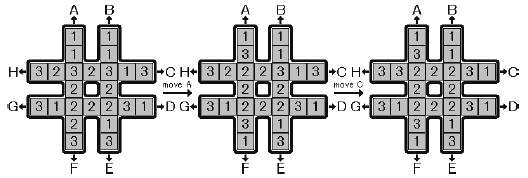
\includegraphics[width=0.5\textwidth]{Images/5070.png}
    \end{center}

    다음은 이 퍼즐에 대한 설명이다.
    \begin{itemize}
        \item 각 블록에는 1부터 3까지 수 중 하나가 적혀 있으며 각각은 정확히 8개씩 있다.
        \item 목표는 가운데 정사각형의 여덟 블록이 모두 같은 숫자가 되도록 하는 것이다.
        \item 사용할 수 있는 동작은 7개의 블록으로 이루어진 줄에서 끝 블록을 반대쪽 끝으로 이동시키고 나머지 여섯 개의 블록을 한 칸씩 미는 8가지의 동작이다. 각각의 동작은 A~H까지 라벨링되어 있다.
    \end{itemize}
    최소 횟수로 동작을 사용하여 퍼즐을 해결하려고 한다. 최소 횟수로 해결하는 방법들 중 사전순으로 가장 앞선 동작의 나열을 출력하고, 그 나열을 쓸 때 가운데 정사각형의 여덟 블록이 어떤 숫자가 되는지 출력하라.
\end{problem}

\begin{problem}
    (25795번) 화이트 초콜릿 조각과 다크 초콜릿 조각을 각각 $N$개를 붙여 초콜릿을 만들었다. 이 나열 중 특별한 조건을 만족하는 초콜릿을 예쁜 초콜릿이라고 한다.
    \begin{itemize}
        \item 화이트 + 다크 는 예쁜 초콜릿이다.
        \item 화이트 + 예쁜 초콜릿 + 다크 는 예쁜 초콜릿이다.
        \item 예쁜 초콜릿 + 예쁜 초콜릿 은 예쁜 초콜릿이다.
        \item 위 세 가지 규칙으로 만들어지지 않는 나머지 초콜릿은 예쁜 초콜릿이 아니다.
    \end{itemize}
    초콜릿의 점수는 정수 $a$에서 시작해 왼쪽부터 화이트 초콜릿 조각이 있으면 $b$를 더하고 다크 초콜릿 조각이 있으면 $c$를 곱하여 계산한 값을 $10^5$으로 나눈 나머지이다. $N, a, b, c$가 주어질 때 예쁜 초콜릿들 초콜릿의 점수가 가장 높을 때 최댓값을 구하여라. $N \leq 15$이고 $a, b, c$는 모두 $10^5$ 이하이다.
\end{problem}

\section{연습문제 C}

\begin{problem} 
    (2071번) $N \times N$의 검은 돌만 놓여 있는 바둑판의 집의 개수를 세려고 한다. 기존의 바둑과 다르게 모든 방향에서 블록으로 가려져 있는 곳만을 집으로 인정한다. 즉, 테두리는 둘러싸일 수 없으므로 집이 아니다. 하지만 바둑판을 이미 치워 바둑판의 모양은 알 수 없고 각 $N$개의 가로줄과 세로줄에 있는 바둑돌의 수, 각 $2N-1$개의 우상향과 우하향 방향의 대각선에 있는 바둑돌의 수만을 알고 있다. 이 정보를 입력으로 받아 바둑판에 있는 집의 크기를 계산하는 프로그램을 작성하라. 단, $N \leq 15$이고 주어진 정보로 바둑판의 모양을 유일하게 결정할 수 있음이 보장된다.
\end{problem}

\begin{problem}
    (2396번) 길이가 $L$인 막대 $M$개를 잘라 토막 $N$개를 얻었다. 다시 이 토막으로 길이가 같은 막대 여러 개를 만드려고 한다. 가능한 방법들 중에서 토막의 길이가 가장 짧을 때 그 길이를 출력하라. $N \leq 100$이고 토막의 길이도 $100$ 이하이다.
\end{problem}

\begin{problem}
    (18461번**) 길이가 $N$인 순열(permutation)에서 최장 증가 부분 수열(LIS)과 같은 길이를 가지며 교집합이 공집합인 증가하는 부분 수열 두 개가 존재하는 순열의 개수를 구하여라. $N \leq 75$이다.
    \begin{itemize}
        \item 길이가 $N$인 순열은 $1$부터 $N$까지의 수가 정확히 한 번씩 나타나는 수열이다.
        \item 증가 부분 수열은 길이 $N$의 주어진 수열에서 몇 개의 수를 제거하여 만든 증가 수열을 말하고, 최대 증가 부분 수열은 어떤 수열의 증가 부분 수열들 중 가장 긴 길이의 증가 부분 수열이다.
    \end{itemize}
\end{problem}

\begin{problem}
    (24258번*) $n$이 주어질 때 $a_1 a_2 a_3 \cdots a_n = a_1 + a_2 + \cdots + a_n$이며 $a_1 \geq a_2 \geq \cdots \geq a_n$인 순서쌍 $(a_1, a_2, \cdots, a_n)$의 개수를 출력하라. $2 \leq n \leq 10^{11}$이고 이러한 순서쌍의 개수는 주어진 조건에서 $10^{18}$개 미만임이 보장된다.
\end{problem}

\begin{problem}
    (26272번) $N$가지의 참-거짓 질문에 대한 대답 순서쌍이 모두 다른 $2^N$명의 사람들이 있다. 연구원은 매일 피실험자들을 대상으로 $2N$가지 유형의 실험을 진행하는데, $2i-1$번 유형의 실험에서는 $i$번 질문에 참이라 대답한 사람만 부르고, $2i$번 유형의 실험에서는 $i$번 질문에 거짓이라 대답한 사람만 부른다. 피실험자의 편의를 위해 연구원들은 이전 실험에 참가한 피실험자들 중 절반 이상이 다음 실험의 참여 대상이 되도록 순서를 정하려고 한다. 하지만 매번 실험 순서가 같다면 실험이 편향될 수 있기 때문에 연구자들은 $x$번 유형의 실험을 $y$번째로 시행할 수 있는 실험 시행 순서 중 가장 사전순으로 앞선 것을 택할 것이다. 여러분은 $Q$번 $x$와 $y$가 주어질 때마다 결정되는 실험 시행 순서 $a_k$를 구해 
    $$\sum_{k=1}^{2N} {ka_k}$$
    를 $10^9 + 7$로 나눈 나머지를 출력해야 한다. $2 \leq N \leq 10^9$이고, $1 \leq Q \leq 2\cdot10^5$이다.
\end{problem}

\newpage

\section{힌트}

\begin{hint}

\end{hint}

\begin{hint}

\end{hint}

\begin{hint}

\end{hint}

\begin{hint}
    thregium의 practice\_baekjoon 레포지토리
\end{hint}

\begin{hint}
    두 가지 최적화가 필요하다.
    \begin{itemize}
        \item 똑같은 무게를 가지는 여러 물건들 중에서 ?한 것을 먼저 골라야 한다.
        \item $C$ 이하인 가장 큰 피보나치 수부터 $t_1, t_2, \cdots$라 하면, 적당히 작은 상수 $k$에 대해 무게가 $t_1, t_2, \cdots, t_k$인 물건을 모두 고르지 않으면 [...]을 보장할 수 있다.
    \end{itemize}
\end{hint}

\begin{hint}
    N-Queen 문제와 비슷하게, 한 대각선에는 하나의 비숍만 놓일 수 있음을 활용해보자.
\end{hint}

\begin{hint}
    
\end{hint}

\begin{hint}
    모든 화이트 초콜릿을 자신보다 뒤에 있는 다크 초콜릿과 대응시키되, 모두 다른 다크 초콜릿과 대응시킬 수 있어야 예쁜 초콜릿이다. 이 조건은 현재까지 사용한 화이트 초콜릿의 개수와 다크 초콜릿의 개수로 쉽게 판별할 수 있다.
\end{hint}

\begin{hint}
    utilForever의 BOJ 레포지토리
\end{hint}

\begin{hint}
    hummingbird-12의 boj-solutions 레포지토리
\end{hint}

\begin{hint}
    \url{https://qoj.ac/contest/443}
\end{hint}

\begin{hint}
    총 다섯 개의 단계별 힌트가 있다.

    \textbf{[ 1 ]} \newline
    $i \geq j$인 $i$와 $j$에 대해 $(a_i, a_j)$에서 $(a_i+1, a_j-1)$로 바꾸면, 합은 일정하지만 곱은 감소한다. 즉, 합이 일정한 상황에서 곱의 최소는 $(a_1, 1, 1, \cdots, 1)$에서 갖는다. 그런데, $(a_1, 1, 1, \cdots, 1)$에서는 항상 합이 곱보다 크기 때문에, 실질적으로 $(a_1, 2, 1, \cdots, 1)$을 고려해야 한다. 이 상태에서 합보다 곱이 크다면 불가능하다. 이를 수식으로 풀면,
    $$2a_1 \leq n + a_1 \Rightarrow a_1 \leq n, a_1 \times a_2 \times \cdots \times a_n = a_1 + a_2 + \cdots + a_n \leq 2a_1 \leq 2n$$
    가 된다.

    \textbf{[ 2 ]} \newline
    이제, $a_2$부터 하나씩 결정하되, 곱으로 경우의 수를 줄일 것이기 때문에 $2$ 이상의 값으로 결정하자. 그러면 $2$ 이상의 값의 개수가 $2$개일 때부터($1$개는 불가능하다) $n$개일 때까지 모두 확인해야 하므로, 매번 아직 결정되지 않은 값을 모두 $1$로 두고 가능한 $a_1$이 존재하는지 판단하자. 재귀함수의 파라미터로는 $a_k$를 결정할 때의 $k$, $a_k$의 상한, 현재까지 합, 현재까지 곱을 넣으면 충분하다.

    \textbf{[ 3 ]} \newline
    \underline{곱에서 합을 뺀 값}을 점점 작아지게 만들어보자. 아래 부등식에서 각 순서쌍은, 곱에서 합을 뺀 값을 나타낸다.
    
    \begin{align*}
        (a_1, a_2, \cdots, a_n) \geq (a_1 + S, a_2, \cdots, a_k, 1, 1, \cdots, 1) \geq (a_1, a_2, \cdots, a_k, 1, 1, \cdots, 1) & \\ \textrm{where}~S = (a_{k+1}-1) + (a_{k+2}-1) + \cdots + (a_n-1) &
    \end{align*}

    즉, $a_k$까지 수를 정하고 그 이후는 $1$이라 가정한 뒤 가능한 $a_1$을 구했을 때, $a_2$보다 작으면 그 이후는 무조건 불가능하다. $(a_1=a_2, a_2, \cdots, a_k, 1, 1, \cdots, 1)$에서 곱에서 합을 뺀 값이 이미 양수이기 때문에, $(a_1 \geq a_2, a_2, \cdots, a_k, 1, 1, \cdots, 1)$에서도 양수이고, $(a_1, a_2, \cdots, a_k, a_{k+1}, \cdots, a_n)$에서도 양수가 되기 때문이다.

    \textbf{[ 4 ]} \newline
    \textbf{[ 3 ]}에 의해 $a_{k+1}$부터 전부 1일 때 가능한 유리수 $a_1$의 값이 $a_1$의 상한이 된다. 그리고 \textbf{[ 1 ]}에 의해 그 때 $a_1 + a_2 + \cdots + a_n$이 최대이다. 이렇게 구한 합의 상한과 하한 안에, $a_2 \times a_3 \times \cdots \times a_k$의 배수가 있어야 한다. 이를 활용하면 경우의 수를 더 줄일 수 있다.

    \textbf{[ 5 ]} \newline
    \textbf{[ 2 ]}를 확장해, $a_3$부터 하나씩 결정할 수 있다. 이 풀이의 장점은 현재까지의 곱에 따라 두 가지 방법을 사용할 수 있다는 것이다. $a_3 a_4 \cdots a_k$가 작을 때는 $a_2$의 상한이 $O \left( \sqrt{\frac{n}{a_3 a_4 \cdots a_k}} \right)$이므로, 가능한 $a_2$에 따라 $a_1$을 구한다. 반면, $a_3 a_4 \cdots a_k$가 클 때는 \textbf{[ 4 ]}와 같이 $a_1 + a_2 + \cdots a_n$의 값의 상한과 하한을 구하고, 그 범위에 속하는 $a_3 a_4 \cdots a_k$의 배수마다 이차방정식의 근의 공식으로 $a_1$과 $a_2$를 한번에 구하는 것이다. 이 방법은 $O(n \times (a_3 a_4 \cdots a_k)^{-2})$의 시간을 요구한다.
    
    \url{https://old.infosbg.com/Shumen_2021.html}
\end{hint}

\begin{hint}
    이 문제는 직접 규칙을 찾으며 주어진 입력에 따라 케이스를 나누어 수학적으로 해결할 수도 있다. 하지만, 여기서는 백트래킹 풀이에 대한 힌트를 수록한다.

    \textbf{[ 1 ]} \newline
    직전 점호 인원 중 절반이 넘게 소집해제되지 않는다는 것과, $a_k$와 $a_{k+1}$을 $2$로 나눈 몫이 다름은 동치이다.

    \textbf{[ 2 ]} \newline
    만약, $x$번 유형의 점호를 $y$번째로 실시해야 한다는 조건이 없다면, $1, 3, 2, 4, \cdots$와 같은 순서로 두는 것이 사전 순으로 가장 앞선다.

    \textbf{[ 3 ]} \newline
    \textbf{[ 2 ]}의 순서에서 $x$번 유형의 점호를 $y$번째로 실시하기 위해 원래 $x$번 유형이 있던 자리 주변과 $y$번째 주변의 순서를 바꾸어야 할 것이다. 각각에서 사전순 최소를 백트래킹으로 탐색하자.
\end{hint}

\chapter{정렬}
정렬(sorting)은 어떤 배열의 값들을 작은 수부터 큰 수 또는 큰 수부터 작은 수의 순서로 나열하는 것을 말한다. 이 장에서는 총 7가지 정렬 알고리즘과 정렬 기준 설정에 대해 배울 것이다.

\section{비교 기반 정렬 알고리즘}
비교 기반 정렬 알고리즘은 어떤 두 수를 비교해 얻은 결과만을 이용해 정렬하는 알고리즘이다. 다른 말로, 배열 $arr$에 속하는 어떤 두 수 $x, y$를 비교해 더 작은 수가 앞에 와야 함을 이용해 정렬하는 것이다.

이러한 비교 기반 정렬 알고리즘의 특징은 시간복잡도의 상한이 $O(N \log N)$이라는 것이다. 그 이유는 $N$개의 데이터에서 존재할 수 있는 모든 초기 데이터가 $N!$가지인데, 적절한 한 번의 비교를 통해 가능한 경우의 수를 절반으로 줄일 수 있기 때문에 최소 연산 횟수는 $O(\log N!)$로 정해져 있기 때문이다(스털링 근사에 의해 $O(N!)=O(N \log N)$이 된다). 

이 절에서는 총 다섯 종류의 비교 기반 정렬 알고리즘을 다룬다. 앞 3개는 평균 시간복잡도가 $O(N^2)$인 알고리즘, 뒤 2개는 평균 시간복잡도가 $O(N \log N)$인 알고리즘이다. 비교 기반 정렬 알고리즘은 모두 중요하므로 주의 깊게 보도록 하자.

\subsection{버블 정렬}
버블 정렬은 인접한 두 수를 비교해 큰 수가 앞에 있으면 뒤집는 과정을 반복함으로써 정렬하는 방식이다. 정확히 말하면 $1 \leq i < N$인 모든 $i$에 대해 $i$번째 수와 $i+1$번째 수의 크기 순서가 반대이면 $i$번째 수와 $i+1$번째 수를 뒤집는 과정을 정렬될 때까지 반복하는 것이다. \Cref{code: bubble}에 구현 코드가 있다.

\begin{code} \label{code: bubble}
버블 정렬 구현 코드
\begin{lstlisting}
#include <bits/stdc++.h>
using namespace std;

int n, arr[1010];

bool check() {
    for (int i = 1; i < n; i++) {
        if (arr[i] > arr[i + 1]) return true;
    }
    return false;
}

int main() {
    cin >> n;
    for (int i = 1; i <= n; i++) cin >> arr[i];

    while (check()) {
        for (int i = 1; i < n; i++) {
            if (arr[i] > arr[i + 1]) swap(arr[i], arr[i + 1]);
        }
    }

    for (int i = 1; i <= n; i++) cout << arr[i] << " ";
    return 0;
}
\end{lstlisting}
\end{code}

버블 정렬의 시간복잡도는 어떻게 될까? 뒤집는 과정이 반복되는 횟수에 $N$을 곱한 것이 시간복잡도가 될 것이다. 그렇다면 뒤집는 과정은 얼마나 많이 반복될까? 수학적으로 $N$번 이하임을 증명할 수 있다. 즉, 버블 정렬의 시간복잡도는 $O(N^2)$이다. 증명은 \Cref{pb: bubble-pf}을 참고하라.

버블 정렬의 교환 횟수는 어떻게 될까? 한 번 교환할 때마다 $i<j$이고 $arr[i]>arr[j]$인 순서쌍 $(i, j)$의 개수가 하나씩 줄어든다는 것은 자명한 사실이다. 즉, 어떤 배열 $arr$에 대해 $i<j$이고 $arr[i]>arr[j]$인 순서쌍 $(i, j)$의 개수로 정의되는 \textit{Inversion Count}가 버블 정렬의 교환 횟수가 된다. \textit{Inversion Count}를 구하는 문제를 \Cref{pb: inversion-square}에서 풀어보라.

\subsection{삽입 정렬}
삽입 정렬은 앞에서부터 정렬해나가는 방식으로 $x$번째까지 정렬되어 있을 때 $x+1$번째를 자신보다 작은 수가 나올 때까지 앞으로 한 칸씩 옮기며 정렬하는 방식이다. 이 방법을 사용했을 때 정렬이 됨은 자명하게 확인할 수 있다. \Cref{code: insertion}를 보라.

\begin{code} \label{code: insertion}
삽입 정렬 구현 코드
\begin{lstlisting}
#include <bits/stdc++.h>
using namespace std;

int n, arr[1010];

int main() {
    cin >> n;
    for (int i = 1; i <= n; i++) cin >> arr[i];

    for (int i = 1; i <= n; i++) {
        for (int j = i; j >= 2; j--) {
            if (arr[j] < arr[j - 1]) swap(arr[j], arr[j - 1]);
            else break;
        }
    }

    for (int i = 1; i <= n; i++) cout << arr[i] << " ";
    return 0;
}
\end{lstlisting}
\end{code}

삽입 정렬의 재미있는 특징은 거의 정렬되어 있다면 빠른 시간에 완료된다는 것이다. 왜냐하면 $x$번째 수 앞에 있는 수들 중 $x$번째 수보다 큰 수의 개수와 교환 횟수가 동일하기 때문이다($N=5$일 때 배열 $1, 3, 5, 4, 2$와 $5, 4, 3, 2, 1$의 교환 횟수를 비교해 확인해보라). 이러한 특징은 전체 배열이 거의 정렬되었을 때 의도적으로 삽입 정렬을 사용하는 하이브리드 정렬에 자주 사용된다. 하지만 여전히 시간복잡도는 $O(N^2)$이다. 완전히 역순인 최악의 경우에는 교환 횟수가 $N(N-1)/2$이기 때문이다.

\subsection{선택 정렬}
선택 정렬은 배열에서 최솟값을 찾고 그 수를 제일 앞으로 보내는 과정을 반복함으로써 정렬하는 방식이다. 당연히 $k$개의 수를 앞으로 보냈다면 $k+1$번째 수부터 최솟값을 찾아야 한다. \Cref{code: selection}을 보라.

\begin{code} \label{code: selection}
선택 정렬 구현 코드
\begin{lstlisting}
#include <bits/stdc++.h>
using namespace std;

int n, arr[1010];

int main() {
    cin >> n;
    for (int i = 1; i <= n; i++) cin >> arr[i];

    for (int i = 1; i <= n; i++) {
        int idx, val = 1e9;
        for (int j = i; j <= n; j++) {
            if (val > arr[j]) {
                idx = j;
                val = arr[j];
            }
        }
        swap(arr[i], arr[idx]);
    }

    for (int i = 1; i <= n; i++) cout << arr[i] << " ";
    return 0;
}

\end{lstlisting}
\end{code}

시간복잡도는 $O(N^2)$이다.

\subsection{퀵 정렬}
퀵 정렬은 어떤 기준값인 \texttt{pivot}을 잡아 \texttt{pivot}보다 작은 수는 앞으로 보내고, 큰 수는 뒤로 보낸 후 각 부분을 다시 정렬하는 재귀적 정렬 방식이다. 

그렇다면 어떻게 \texttt{pivot}을 기준으로 양쪽으로 수를 나눌까? 일단 \texttt{pivot}의 경우에는 어떤 수를 선택해도 상관없기 때문에, 보통 첫 번째 수를 잡는다. 이후, 두 개의 포인터(정확히는 인덱스 번호를 저장하는 정수형 변수이다) \texttt{p, q}를 사용하는데, \texttt{p}는 왼쪽 끝에서 오른쪽 끝으로, \texttt{q}는 오른쪽 끝에서 왼쪽 끝으로 이동할 것이다. 

매 반복마다 \texttt{p}는 $arr[p]$가 \texttt{pivot}보다 커질 때까지, \texttt{q}는 $arr[q]$가 \texttt{pivot}보다 작아질 때까지 이동한다. 그러면 두 가지 경우가 가능하다:
\begin{itemize}
    \item \texttt{p}와 \texttt{q}의 순서가 뒤집힌 경우에는 분리가 끝났다는 뜻이다. 따라서  기준값인 \texttt{pivot}가 중간에 오도록 \texttt{q}번째 수와 \texttt{pivot}를 바꾼다. \texttt{q}번째 수와 바꾸는 이유는 \texttt{q}번째 수가 \texttt{pivot}보다 작기 때문이다.
    \item \texttt{p}와 \texttt{q}의 순서가 뒤집히지 않은 경우에는 분리가 끝나지 않은 경우이다. 이 경우에는 단순히 \texttt{p}번째 수와 \texttt{q}번째 수를 바꾸어 분리가 되도록 한다.
\end{itemize}
이 과정을 구현한 것이 \Cref{code: quicksort}이다.

\begin{code} \label{code: quicksort}
퀵 정렬 구현 코드
\begin{lstlisting}
#include <bits/stdc++.h>
using namespace std;

int n, arr[1010];

void quicksort(int st, int ed) {
    if (st >= ed) return;
    int pivot = st;
    int lt = st + 1, rt = ed;

    while (true) {
        while (lt <= ed && arr[lt] <= arr[pivot]) lt++;
        while (rt > st && arr[rt] >= arr[pivot]) rt--;
        if (lt > rt) {
            swap(arr[pivot], arr[rt]);
            break;
        }
        else swap(arr[lt], arr[rt]);
    }

    quicksort(st, rt - 1);
    quicksort(rt + 1, ed);
}

int main() {
    cin >> n;
    for (int i = 1; i <= n; i++) cin >> arr[i];

    quicksort(1, n);

    for (int i = 1; i <= n; i++) cout << arr[i] << " ";
    return 0;
}

\end{lstlisting}
\end{code}

이 알고리즘의 시간복잡도는 어떻게 될까? 결론만 말하면 재귀 함수가 재귀적으로 호출된 횟수(재귀의 깊이라고 한다)와 \texttt{pivot}를 기준으로 나누기 위해 필요한 연산 횟수의 곱이 시간복잡도이다(\Cref{pb: quick-merge-time} 참고). 평균적으로 재귀의 깊이는 $O(\log N)$일 것이고, 나누는 과정의 시간복잡도는 $O(N)$이므로 평균 시간복잡도는 $O(N \log N)$이다. 하지만, 최악의 경우 재귀의 깊이는 $O(N)$이므로 최악 시간복잡도는 $O(N^2)$가 된다.

\subsection{병합 정렬} \label{sec: mergesort}
병합 정렬은 가운데 값을 기준으로 양쪽 배열을 정렬한 후 양쪽의 결과를 바탕으로 합쳐 정렬된 배열을 만드는 방식이다. 양쪽 배열이 정렬되어 있기 때문에 다음 관찰이 성립한다.

\begin{obs}
    합쳐진 배열의 첫 번째 수는 왼쪽 배열의 첫 번째 수와 오른쪽 배열의 첫 번째 수 중 작은 수이다.
\end{obs}

이 관찰을 반복적으로 적용할 수 있는데, 왜냐하면 첫 번째 수를 빼고 나머지 두 배열을 합친 결과가 정렬된 배열이 되기 때문이다. 따라서 왼쪽 배열의 현재 수와 오른쪽 배열의 현재 수를 나타내는 포인터(인덱스) \texttt{p}와 \texttt{q}를 이용해 구현할 수 있다. $lt[p]$와 $rt[q]$ 중 작은 수를 넣고 작은 쪽의 포인터를 오른쪽으로 한 칸 움직이면 된다.

\begin{code} \label{code: mergesort}
병합 정렬 구현 코드
\begin{lstlisting}
#include <bits/stdc++.h>
using namespace std;

int n, arr[1010];

void mergesort(int st, int ed) {
    if (st >= ed) return;

    int mid = (st + ed + 1) / 2;
    mergesort(st, mid - 1);
    mergesort(mid, ed);

    vector<int> temp;
    int p = st, q = mid;

    while (true) {
        if (p >= mid && q > ed) break;
        if (p >= mid) {
            temp.push_back(arr[q]);
            q++;
            continue;
        }
        if (q > ed) {
            temp.push_back(arr[p]);
            p++;
            continue;
        }
        if (arr[p] <= arr[q]) {
            temp.push_back(arr[p]);
            p++;
        }
        else {
            temp.push_back(arr[q]);
            q++;
        }
    }

    for (int i = st; i <= ed; i++) arr[i] = temp[i - st];
}

int main() {
    cin >> n;
    for (int i = 1; i <= n; i++) cin >> arr[i];

    mergesort(1, n);

    for (int i = 1; i <= n; i++) cout << arr[i] << " ";
    return 0;
}

\end{lstlisting}
\end{code}

뒤에서 다시 배우겠지만, 이렇게 구간을 분할한 후 다시 합치는 과정을 통해 문제를 해결하는 방법을 분할 정복(divide and conquer)라고 한다. 병합 정렬은 대표적인 분할 정복 알고리즘의 예시이다.

병합 정렬은 퀵 정렬과 다르게 항상 배열의 길이가 절반이 됨이 보장된다. 따라서 재귀의 깊이는 최악의 경우에도 $O(\log N)$이므로 최악 시간복잡도도 $O(N \log N)$이다.

\section{정수 정렬 알고리즘}
정수 정렬 알고리즘은 모든 값이 정수일 때 비교가 아닌 다른 방식으로 정렬하는 방법으로, 정수의 특징을 이용하는 경우가 많다. 이 정수 정렬 알고리즘의 아이디어는 다양한 문제에서 사용될 수 있으므로 꼭 한 번 구현해보는 것을 추천한다.

\subsection{계수 정렬}
계수 정렬은 값의 개수를 저장한 후 작은 값부터 그 값의 개수만큼 새로운 배열에 추가함으로써 정렬하는 방식이다.

\begin{code}
계수 정렬 구현 코드
\begin{lstlisting}
#include <bits/stdc++.h>
using namespace std;

int n, arr[1010], cnt[1010];
const int x = 1000;

int main() {
    cin >> n;
    for (int i = 1; i <= n; i++) cin >> arr[i];

    for (int i = 1; i <= n; i++) cnt[arr[i]]++;

    vector<int> res;
    for (int i = 1; i <= x; i++) {
        for (int j = 1; j <= cnt[i]; j++) res.push_back(i);
    }

    for (int i = 0; i < n; i++) cout << res[i] << " ";
    return 0;
}
\end{lstlisting}
\end{code}

이전까지의 정렬과 다르게 \texttt{cnt[]} 배열을 선언해 개수를 저장해야 한다. 따라서 \texttt{cnt[]} 배열의 인덱스 개수는 최댓값 $X$ 이상이어야 하고, 공간복잡도가 값의 크기에 영향을 받게 된다. 또한, 반복문이 $1$부터 $X$까지 진행되며 $cnt[i]$개 만큼 $i$를 추가하는 과정이 포함되므로 시간복잡도도 값의 크기에 영향을 받게 된다.

이제 시간복잡도를 계산해보자. $cnt[i]$의 최댓값은 $N$이고, $i$를 총 $X$개 확인해야 하므로 $O(NX)$일까? 하지만, 실제로 \texttt{res}에 값이 추가되는 횟수는 $cnt[i]$의 총 합이 $N$이므로 $N$번이다. 즉, $i$에서 $cnt[i]$가 $N$일 수 없다. 따라서 다음과 같이 계산해야 정확히 시간복잡도를 구할 수 있다.

$$O\left(\sum_{i=1}^X {(1+cnt[i])}\right) = O(N+X)$$

결론적으로 시간복잡도 $O(N+X)$, 공간복잡도 $O(N+X)$가 된다.

\subsection{기수 정렬}
기수 정렬은 정수의 중요한 성질인 진법을 활용한다. 각 정수를 진법을 통해 자리수로 나누어 저장하고, 낮은 자리수부터 계수 정렬의 원리를 활용하여 정렬하는 방식이다.

먼저 필요한 자리수 $d$를 계산한다. 이후 각 자리수에 대해 다음을 반복한다.
\begin{itemize}
    \item $i$번째 자리수를 계산한다. 15번째 줄을 참고하라.
    \item $j$번째 수의 $i$번째 자리수가 $t$이면 \texttt{cnt[t]}에 $j$를 추가한다. 개수를 저장하지 않고 인덱스를 저장하는 이유는 $t$는 실제 배열 $arr$에 포함된 수가 아니기 때문이다.
    \item $i$번째 자리수가 작은 것부터 \texttt{cnt[t]} 배열에 저장된 인덱스를 이용해 새로운 배열 \texttt{res}에 추가한다. 이후 \texttt{res}의 값을 \texttt{arr}에 대입한다.
\end{itemize}

다음 \Cref{code: radixsort}은 위 알고리즘을 구현한 것이다.

\begin{code} \label{code: radixsort}
기수 정렬 구현 코드
\begin{lstlisting}
#include <bits/stdc++.h>
using namespace std;

int n, arr[1010], cnt[1010];
const int x = 1000, r = 10;

int main() {
    cin >> n;
    for (int i = 1; i <= n; i++) cin >> arr[i];

    double d = log(x)/log(r);
    for (int i = 0; i <= d; i++) {
        vector<int> cnt[r], res;
        for (int j = 1; j <= n; j++) {
            int t = (arr[j] % (int)pow(r, i+1)) / (int)pow(r, i);
            cnt[t].push_back(j);
        }
        for (int k = 0; k < r; k++) {
            for (int j = 0; j < (int)cnt[k].size(); j++) 
                res.push_back(arr[cnt[k][j]]);
        }
        for (int j = 1; j <= n; j++) arr[j] = res[j - 1];
    }

    for (int i = 1; i <= n; i++) cout << arr[i] << " ";
    return 0;
}

\end{lstlisting}
\end{code}

주의해야 할 점은 이미 이전 자리수를 기준으로 정렬된 순서가 깨지면 안된다는 점이다. 같은 $t$를 갖더라도 그 앞 자리 수가 작은 수가 더 앞에 와야 하기 때문이다. 이러한 정렬을 안정 정렬(stable sorting)이라고 하며, 기수 정렬에서 사용되는 계수 정렬은 무조건 안정 정렬이어야 한다.

기수 정렬의 시간복잡도와 공간복잡도는 계수 정렬과 비슷하게 구할 수 있다. \Cref{pb: radix-time}을 참고하라.

\section{내장 정렬 함수 사용하기}
C++의 표준 템플릿 라이브러리(STL)에는 내장 정렬 함수 \texttt{std::sort}가 있다. \texttt{std::sort(start, end, compare)}로 정의되며, \texttt{start}는 시작 포인터, \texttt{end}는 끝 포인터, \texttt{compare}은 비교 기준을 나타내는 함수 포인터이다. 즉, $[\texttt{start}, \texttt{end})$ 구간을 \texttt{compare}을 기준으로 정렬해준다. \url{https://en.cppreference.com/w/cpp/algorithm/sort}에서 제공하는 예시 코드를 이용해 구체적으로 설명하겠다.

\begin{code} \label{code: stdsort}
\texttt{std::sort} 예시 코드
\begin{lstlisting}
#include <algorithm>
#include <array>
#include <functional>
#include <iostream>
#include <string_view>
 
int main()
{
    std::array<int, 10> s {5, 7, 4, 2, 8, 6, 1, 9, 0, 3};
 
    auto print = [&s](std::string_view const rem)
    {
        for (auto a : s)
            std::cout << a << ' ';
        std::cout << ": " << rem << '\n';
    };
 
    std::sort(s.begin(), s.end());
    print("sorted with the default operator<");
 
    std::sort(s.begin(), s.end(), std::greater<int>());
    print("sorted with the standard library compare function object");
 
    struct
    {
        bool operator()(int a, int b) const { return a < b; }
    }
    customLess;
 
    std::sort(s.begin(), s.end(), customLess);
    print("sorted with a custom function object");
 
    std::sort(s.begin(), s.end(), [](int a, int b)
                                  {
                                      return a > b;
                                  });
    print("sorted with a lambda expression");
}
\end{lstlisting}

\end{code}

\begin{itemize}
    \item \texttt{compare} 함수를 빈칸으로 놓으면 기본 \texttt{<} 연산자에 의해 정렬된다.
    \item \texttt{compare} 함수로 STD에서 지원하는 비교 함수 객체를 사용할 수 있다. \texttt{std::less<T>}로 놓으면 오름차순으로, \texttt{std::greater<T>}로 놓으면 내림차순으로 정렬된다.
    \item 직접 함수 객체를 정의해 사용할 수 있다. 함수 객체 선언 방식은 24에서 28번 줄을 참고하라.
    \item 람다 표현법으로 직접 \texttt{compare}에 함수를 추가할 수 있다. 람다 표현법은 33에서 36번 줄을 참고하라.
\end{itemize}

추가로, 비교 시 값이 같다면 앞에 있는 수가 정렬된 배열에서도 앞에 오도록 정렬할 수 있다. 이러한 정렬을 안정 정렬(stable sorting)이라고 하며, STL에서는 \texttt{std::stable\_sort}를 사용하면 된다. 함수 사용 방법은 똑같다.

\section{연산자 오버로딩}
내장 정렬 함수에서 \texttt{compare}에 비교 기준을 넣어 원하는 기준에 따라 정렬할 수도 있지만, 연산자 오버로딩(operator overloading)을 사용할 수도 있다. 원하는 비교 기준을 연산자 \texttt{<}에 오버로딩하여 \texttt{compare} 함수를 따로 쓰지 않고 정렬하는 것이다. 다음 \Cref{code: operator-overloading}는 구조체에서 연산자 오버로딩을 통해 정렬하는 예시 코드이다. 구조체에서 연산자 오버로딩을 해야 하는 경우가 생기면 \Cref{code: operator-overloading}를 참고해 \texttt{operator} 함수를 정의하라.

\begin{code} \label{code: operator-overloading}
연산자 오버로딩 예시 코드
\begin{lstlisting}
#include <bits/stdc++.h>
using namespace std;

int n;
struct Data{
    int teamA, teamB;
    bool operator<(const Data &other) const {
        return teamA - teamB < other.teamA - other.teamB;
    }
} arr[1010];

int main() {
    cin >> n;
    for (int i = 1; i <= n; i++) cin >> arr[i].teamA >> arr[i].teamB;

    sort(arr + 1, arr + n + 1);

    for (int i = 1; i <= n; i++) 
        cout << arr[i].teamA << " " << arr[i].teamB << "\n";
    return 0;
}
\end{lstlisting}
\end{code}

\section{순열 얻기}
때로는 정렬된 수열의 어떤 수가, 원래 수열에서 몇 번째에 있었는지 알아야 할 필요가 있다. 다음 예시 문제가 그러하다.

\begin{example}
    (1015번) 길이 $N$인 수열 $A_i$와 순열 $P_i$를 생각하자. 그러면 $A_i = B_{P_i}$가 되도록 길이 $N$인 수열 $B_i$를 유일하게 결정할 수 있다. $A_i$가 주어질 때 $B_i$가 단조증가하도록 만드는 사전 순으로 가장 앞선 $P_i$를 출력하라. $N \leq 50$, $A_i \leq 1000$이다.
\end{example}

중요한 관찰은 $i$번째 수가 정렬된 수열 $B$에서 몇 번째인지 나타내는 수가 $P_i$라는 것이다. 그리고, $P_i$로 가능한 값은 똑같은 수가 존재할 수 있기 때문에 구간으로 나오게 되는데, $P_i$가 사전 순으로 가장 앞서게 하려면 작은 $i$부터 작은 값을 할당해야 한다. 정렬된 배열에서 $a$번째부터 $b$번째까지 값이 모두 $t$로 같다면, $A_i = t$인 모든 $i$에 대해 $P_i \in [a, b]$여야 하고, 이러한 $i$는 정확히 $b-a+1$개이므로 작은 $i$부터 $a, a+1, \cdots$의 순으로 $P_i$를 정하면 된다.

이것을 하려면 정렬된 수열의 어떤 수가 원래 수열에서 몇 번째인지 알아야 한다. \texttt{std::pair} 객체를 활용하면 쉽게 할 수 있다. 아래 코드를 보자.

\begin{lstlisting}
pair<int, int> arr[55];
// ...
    for (int i = 1; i <= n; i++) {
        cin >> arr[i].first;
        arr[i].second = i;
    }
    sort(arr + 1, arr + n + 1);
// ...
\end{lstlisting}

\texttt{std::pair} 객체를 사용해서 정렬하고자 하는 배열을 첫 번째로, 그리고 인덱스를 두 번째로 넣으면, 첫 번째 값을 기준으로 정렬되므로 제대로 정렬이 된다. 그리고 두 번째 값을 읽으면 그 값이 원래 배열에서 어디에 있었는지 알 수 있게 된다.

위 문제에서는 $P_i$가 최소가 되게 해야 하므로, 안정 정렬을 해야 원하는 위치를 나타내는 순열(permutation)을 얻게 된다. 이를 이용하면 문제를 해결할 수 있다.

\section{정렬의 활용}
다음 문제는 정렬이 필요하다.

\begin{example}
    (1059번) 크기 $N$인 집합 $S$에 대해 $n$을 포함하지만 $S$의 그 어떤 원소도 포함하지 않는 서로 다른 닫힌 구간 $[a, b]~(1 \leq a < b)$의 개수를 구하여라. $N \leq 50$이고 $S$의 모든 원소는 $1000$ 이하의 서로 다른 수이며, $n$은 $S$에서 가장 큰 수보다 작거나 같은 자연수이다.
\end{example}

$S = \{5, 10\}$일 때, $S$의 그 어떤 원소도 포함하지 않는 서로 다른 닫힌 구간은 $[1, 4]$에 속하거나, $[6, 9]$에 속하거나, $[10, \infty)$에 속해야 한다. 이 구간들은 겹치지 않기 때문에 결국 $n$을 포함하면서 $S$의 그 어떤 원소도 포함하지 않는 서로 다른 닫힌 구간은 딱 하나의 구간에 속해야 한다.

이 구간을 찾을 때 정렬이 필요하다. $n$ 좌우의 가장 가까운 $S$에 속하는 원소를 찾으면 그것이 구간이 되는데, 정렬하면 $n$이 사이에 들어가는 두 수를 찾으면 각각이 가장 가까운 원소임이 보장되기 때문이다. 이후에는 수학적으로 $n$을 포함해야 함을 고려해 가능한 왼쪽 끝점과 오른쪽 끝점의 경우의 수를 각각 구해 곱하면 답을 얻을 수 있다.

또 다른 문제를 하나 보자.

\begin{example}
    어떤 다항식을 $\sum c_i x^{k_i}~(c_i \neq 0)$로 표현하는 것은 다항식을 최소 개수의 항으로 표현하는 방식이다. 최소 개수의 항으로 표현된 다항식 두 개가 입력으로 주어질 때, 두 다항식의 곱을 최소 개수의 항으로 표현하라.
\end{example}

정렬은 곱한 결과를 최소 개수의 항으로 표현하기 위해 필요하다. 곱셈을 이중 반복문으로 구현하고 만들어지는 항을 차례대로 추가하고, 지수가 같은 두 개 이상의 항을 찾아 하나로 합쳐 주어야 한다. 이를 해결하는 가장 쉬운 방법은 각 항마다 전체를 순회하면서 지수가 같은 다른 항을 모두 찾아 합치는 것이다. 그런데, 지수를 기준으로 정렬하면, \textbf{지수가 같은 항은 항상 인접하게 될 것}이므로 훨씬 더 작은 시간복잡도로 구현할 수 있게 된다.

\section{연습문제 A}
\begin{problem}
    비교 기반 정렬 알고리즘 다섯 가지를 직접 구현하라. 길이 $N \leq 10000$의 같은 랜덤 데이터에 대한 시간을 측정해 분석하라.
\end{problem}
\begin{problem} \label{pb: bubble-pf}
    버블 정렬의 정당성을 증명하라. 증명을 바탕으로 버블 정렬의 시간복잡도가 $O(N^2)$임을 증명하라.
\end{problem}
\begin{problem} \label{pb: inversion-square}
    Inversion Count를 $O(N^2)$의 시간복잡도에 구현하라.
\end{problem}
\begin{problem}
    \Cref{code: insertion}의 13번째 줄의 \texttt{break} 문을 없애면 어떻게 되는가?
\end{problem}
\begin{problem}
    \Cref{code: selection}의 11번째 줄에서 \texttt{val}을 \texttt{1e9}로 설정하였다. \texttt{1e9}가 갖는 의미가 무엇인가?
\end{problem}
\begin{problem} \label{pb: quick-merge-time}
    퀵 정렬이나 병합 정렬과 같은 재귀함수 기반의 알고리즘의 시간복잡도는 어떻게 구할까? 퀵 정렬과 병합 정렬을 예시로 하여 고민해보라.
\end{problem}
\begin{problem}
    퀵 정렬의 시간복잡도는 최악의 경우 $O(N^2)$이다. 이 문제를 해결할 수 있는 개선된 퀵 정렬이 있을까? 직접 생각해보아도 좋고, 검색하여 찾아보아도 좋다.
\end{problem}
\begin{problem}
    \Cref{code: mergesort}의 9번째 줄을 설명하라. \texttt{mid = (st + ed) / 2}로 정의하면 어떻게 될까?
\end{problem}
\begin{problem}
    정수 정렬 알고리즘 두 가지를 직접 구현하라.
\end{problem}
\begin{problem} \label{pb: radix-time}
    값의 개수를 $N$, 값의 범위를 $X$ 이하의 정수, 사용하는 진법을 $r$이라고 할 때, 기수 정렬 알고리즘의 시간복잡도와 공간복잡도를 구하라. 시간복잡도가 $r$의 변화에 따라 어떻게 변하는가?
\end{problem}
\begin{problem}
    위의 7개 정렬 방식 중 안정 정렬인 것은 무엇인가?
\end{problem}
\begin{problem}
    \Cref{code: stdsort}의 실행 결과를 예측하고, 실제로 실행해 확인해보라.
\end{problem}
\begin{problem}
    \Cref{code: operator-overloading}의 \texttt{arr}의 마지막 값은 무엇인가?
\end{problem}

\section{연습문제 B}

\begin{problem}
    (2107번) 수직선에 $N$개의 닫힌 구간 $[a_i, b_i]$가 있다. 또, $a_i$와 $b_i$는 모두 서로 다르다. 즉, 어떤 한 정수는 많아야 한 구간의 끝점이다. 어떤 경우에는 한 구간이 다른 구간에 포함될 수도 있다. 한 구간이 포함하는 다른 구간의 개수의 최댓값을 찾는 프로그램을 작성하라. $N \leq 25000$이고 $1 \leq A_i < B_i \leq 2 \cdot 10^9$이다.
\end{problem}

\begin{problem}
    (4701번) $N$명의 알파벳 이름이 주어질 때, 절반은 $S$보다 사전순으로 뒤이고 절반은 $S$보다 사전순으로 앞이거나 같은 $S$를 찾고 싶다. 이러한 $S$들 중 사전순으로 가장 앞선 $S$를 출력하라. $N \leq 1000$인 짝수이고 알파벳 이름의 길이는 $30$ 이하이다.
\end{problem}

\begin{problem}
    (9078번) 길이 $N$의 주어진 수열이 \textbf{이웃하는 숫자 두 개를 묶어서} 원하는 곳에 넣는 작업만으로 정렬할 수 있는지 판단하는 프로그램을 작성하라. $N \leq 100$이다.
\end{problem}

\begin{problem}
    (17553번*) $N$개의 좌표 $(x, y)$가 주어질 때, $(a, b)$와 $(c, d)$와의 거리가 같은 점은 많아야 1개이며 절반은 $(a, b)$와 더 가깝고 나머지 절반은 $(c, d)$와 더 가까운 $(a, b)$와 $(c, d)$를 하나 정하라. 단, $a, b, c, d$는 모두 절댓값이 $10^{18}$ 이하인 정수여야 한다. $N \leq 10^5$이고 $(x, y)$의 $x$와 $y$는 모두 절댓값이 $10^9$ 이하인 정수이다.
\end{problem}

\begin{problem}
    (21091번*) 길이가 $N$인 두 순열 $A$와 $B$가 주어질 때, 순열 $A$의 부분 구간 $[l, r]$을 오름차순 정렬 또는 내림차순 정렬하는 작업으로 순열 $B$를 만드는 방법 한 가지를 제시하라. 작업 사용 횟수는 $N$번 이하이기만 하면 되고, 최소화할 필요는 없다. $N \leq 500$이다.
\end{problem}

\begin{problem}
    (21112번) 길이가 $N$인 수열을 차이가 $K$ 이하인 수를 바꾸는 것만으로 정렬할 수 있을 $K$의 최솟값을 구하라. $N \leq 2 \cdot 10^5$이고 수열의 원소는 $10^{18}$ 이하의 자연수이다.
\end{problem}

\begin{problem}
    (25323번*) 길이가 $N$인 수열에서 곱이 제곱수인 두 수만을 바꾸어 정렬할 수 있는지 판별하라. $N \leq 5 \cdot 10^5$이고 수열의 원소는 $10^{18}$ 이하의 자연수이다.
\end{problem}

\begin{problem}
    (28076번) 멀티탭의 방향과 꽃는 구멍이 30도 차이나는 멀티탭 $N$개를 생각하자. 다른 말로 하나의 멀티탭 위에 다른 멀티탭을 꽂으면 두 멀티탭 사이의 각도는 60도이다. 멀티탭을 적절히 꽂아 위에서 보았을 때 보이는 멀티탭 칸의 수가 최소가 되도록 할 때, 최솟값을 출력하라. $N \leq 2 \cdot 10^5$이고 멀티탭에 있는 칸 수는 $2$ 이상 $10^8$ 이하의 정수이다.
    
    \begin{center}
        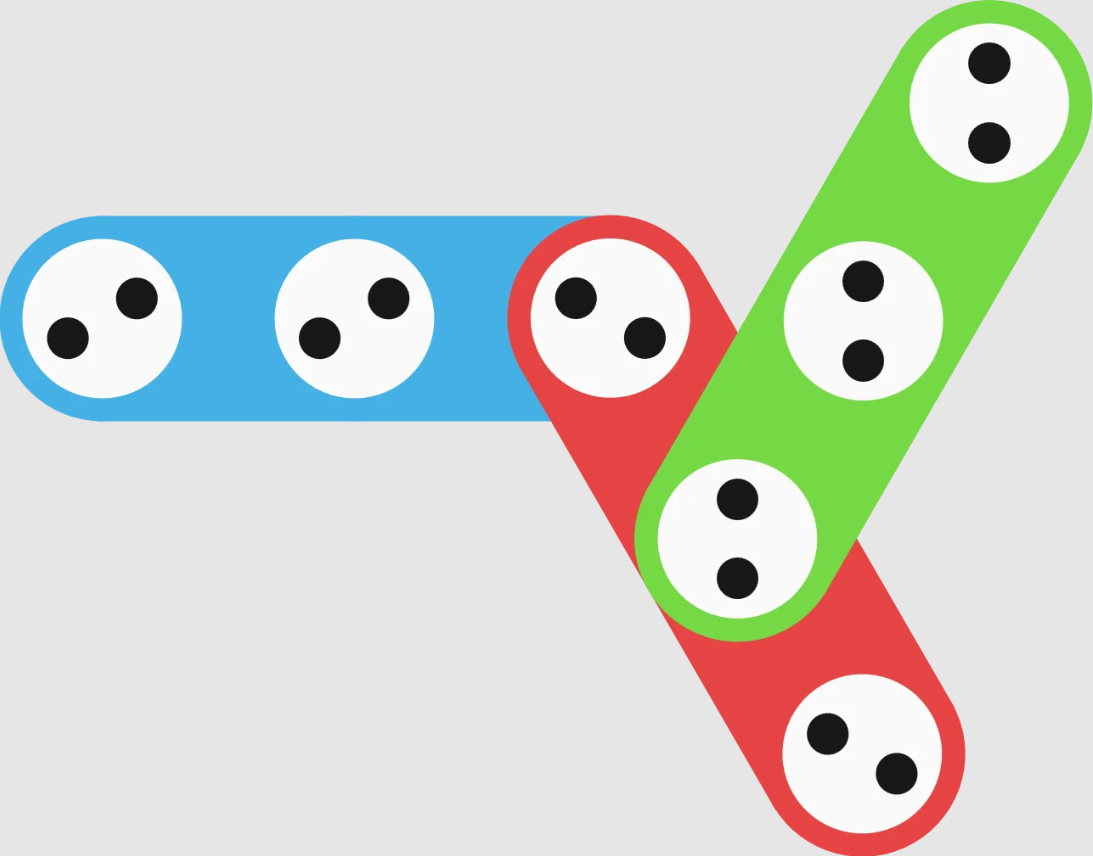
\includegraphics[width=0.5\textwidth]{Images/28076.png}
    \end{center}
\end{problem}

\section{연습문제 C}

\begin{problem}
    (8883번**) 주어진 다각형을 가로 $x_s$, 세로 $y_s$의 직사각형 종이 여러 개로 덮으려고 한다. 이때 종이의 각 변은 $x$축 또는 $y$축과 평행해야 하고 주어진 다각형의 회전은 불가능하다. 오차를 피하기 위해 지도가 종이의 바깥으로 $10^{-6}$까지 나가는 것을 허용한다. 필요한 종이의 수의 최솟값을 구하여라. 다각형의 꼭짓점의 수 $N$은 $3$ 이상 $50$ 이하의 정수이고 지도의 꼭짓점의 좌표 $(x, y)$는 $0 \leq x \leq 10x_s$와 $0 \leq y \leq 10y_x$를 만족한다.
\end{problem}

\begin{problem}
    (10069번*, IOI14) $0$부터 $M-1$까지 번호가 부여된 $M$개의 블록과 북쪽에는 서쪽 방향의 철도, 남쪽에는 동쪽 방향의 철도가 있는 길을 생각하자. 철도 사이의 블록 중 $N$개에는 $0$번부터 $N-1$번까지의 기차역이 하나씩 존재하며, 기차역이 있는 블록에는 북쪽 철로에서 남쪽 철로로 이어지는 세로 방향 철로 또는 남쪽 철로에서 북쪽 철로로 이어지는 세로 방향 철로가 있다. 또한 각 블록을 잇는 수평 방향 철로 사이에는 커넥터가 있다(회색 직사각형).
    
    \begin{center}
        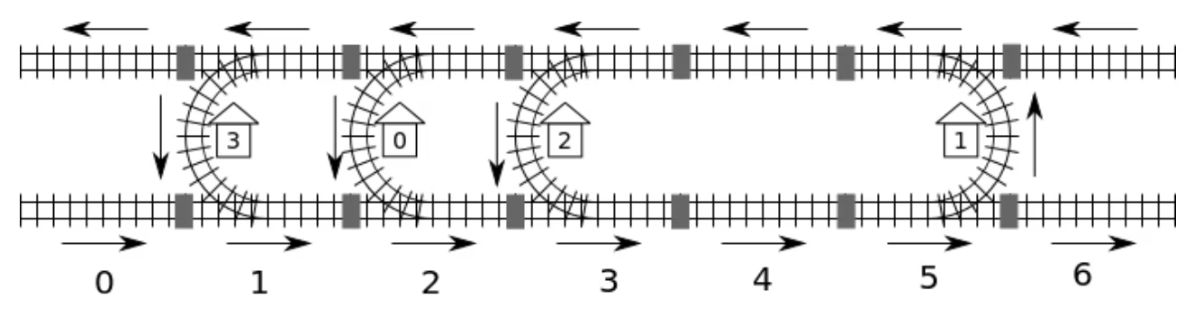
\includegraphics[width=0.8\textwidth]{Images/10069.png}
    \end{center}

    두 역 사이의 최단거리는 두 역 사이를 기차로 이동할 때 지나는 커넥터의 최소 개수이며, 모든 두 역 쌍에 대해 도달할 수 있음이 보장된다. 우리는 $0$번 기차역이 $C$번 블록 위에 있고 $0$번 기차역에 있는 철로의 방향이 북에서 남이라는 사실과 $Q$번의 두 역 사이의 최단거리에 대한 질의만으로 각 역이 있는 블록의 번호와 각 역에 있는 철로의 방향이 북에서 남인지, 남에서 북인지 알아내어야 한다.
    \begin{itemize}
        \item (서브테스크 1) $N \leq 100$이고 $Q$에 제한이 없으며, $0$번 역을 제외하면 나머지 역의 철로 방향은 남에서 북이다.
        \item (서브테스크 2) $N \leq 100$이고 $Q$에 제한이 없으며, $0$번 역의 오른쪽에 있는 철로 방향은 남에서 북이고, 왼쪽에 있는 철로 방향은 북에서 남이다.
        \item (서브테스크 3) $N \leq 5000$이고 $Q$는 $N(N-1)/2$ 이하여야 한다.
        \item (서브테스크 4) $N \leq 5000$이고 $Q$는 $3(N-1)$ 이하여야 한다.
    \end{itemize}

\end{problem}

\begin{problem}
    (10720번) 둘레의 길이가 $L$인 원형 레일을 $L$등분 한 후 각 지점에 $0$부터 $L-1$까지 번호를 붙였다. 그 위에 $N$마리의 시계 방향으로 이동하는 개미와 $M$마리의 반시계 방향으로 이동하는 개미가 있다. 모든 개미의 이동 속도는 초당 $1$이고, 개미는 충돌 이후 반대 방향으로 같은 속도로 이동하게 된다. 모든 개미가 처음과 같은 위치 및 이동 방향을 갖기 위해 필요한 시간 $T$를 출력하라. 단, 모든 개미는 구별되므로, 처음 그 자리에 있었던 개미가 다시 그 자리로 오는 때를 찾아야 한다. $L \leq 600$, $1 \leq N+M \leq 600$, $N \geq 1$, $M \geq 1$이다.
\end{problem}

\begin{problem}
    (15767번**) 이차원 좌표평면에 $N$개의 원이 있다. 다음 과정을 통해 원을 지워나간다.
    \begin{enumerate}
        \item 지워지지 않았고 반지름이 가장 큰 원들 중 인덱스가 가장 작은 원을 찾는다. 이 원을 \textit{target}이라 하자.
        \item \textit{target}과 겹치는 원을 모두 지운다. 겹친다는 것은 두 원의 내부 및 경계의 교집합이 공집합이 아님을 말한다.
    \end{enumerate}
    위 과정을 원이 모두 사라질 때까지 반복하면 각 원은 특정 반복에서 지워진다. 각 원이 지워진 반복에서 \textit{target} 원의 번호를 출력하는 프로그램을 작성하라. $N \leq 3 \cdot 10^5$이고 원의 중심 좌표는 절댓값이 $10^9$ 이하의 정수, 원의 반지름은 $10^9$ 이하의 자연수이다.
\end{problem}

\begin{problem}
    (18480번**) 겹치지 않는($r_i < l_{i+1}$) $N$개의 닫힌 구간 $[l_i, r_i]$의 합집합 $A$에 대해 크기가 $4$인 $A$의 부분집합들 중 합이 $s$인 부분집합의 개수를 구하여라. $N \leq 400$, $0 \leq s \leq 8 \times 10^8$, $0 \leq l_i \leq r_i \leq 2 \cdot 10^8$이다.
\end{problem}

\begin{problem}
    (18738번**) $1$부터 $2N$까지의 숫자가 정확히 한 번씩 적힌 $2N$장의 카드를 두 플레이어가 $N$장씩 나누어 갖는다. 그리고 다음과 같은 규칙으로 게임을 한다.
    \begin{itemize}
        \item 홀수번째 라운드에서는 선 플레이어가 먼저 카드를 내고, 짝수번째 라운드에서는 후 플레이어가 먼저 카드를 낸다.
        \item 각 라운드에서 두 번째로 카드를 내는 플레이어는 상대방이 낸 카드보다 큰 숫자가 적힌 카드를 1개 이상 갖고 있다면 그러한 카드(들) 중 하나를 내야 한다.
        \item 각 라운드에서 더 큰 숫자를 낸 플레이어가 그 라운드를 승리한다.
        \item 각 라운드에서 제출한 카드는 제거된다.
    \end{itemize}
    선 플레이어와 후 플레이어가 받은 $N$장의 카드가 각각 주어질 때, 선 플레이어가 이길 수 있는 라운드의 수의 최댓값을 구하여라. $N \leq 1000$이다.
\end{problem}

\newpage

\section{힌트}
\begin{hint}
    
\end{hint}
\begin{hint}
    정렬의 정의로 `모든 $i$와 $n>0$에 대해 $arr[i] < arr[i + n]$'를 사용하라.
\end{hint}
\begin{hint}
    Inversion Count가 무엇과 같다고 했었는지 생각해보라.
\end{hint}
\begin{hint}
    
\end{hint}
\begin{hint}
    
\end{hint}
\begin{hint}
    
\end{hint}
\begin{hint}
    
\end{hint}
\begin{hint}
    
\end{hint}
\begin{hint}
    
\end{hint}
\begin{hint}
    
\end{hint}
\begin{hint}
    
\end{hint}
\begin{hint}
    
\end{hint}
\begin{hint}
    
\end{hint}

\begin{hint}
    $N^2$ 알고리즘을 짜기에 $N$이 크다고 생각할 수 있지만, 단순 연산은 상수가 작아 시간 안에 돌기 충분하다.
\end{hint}

\begin{hint}
    기본적으로 케이스에 따라 분류해서 풀어야 하는데, 예외 케이스가 많아서 틀리기 쉽다. 그나마 쉬운 구현 방법은, 답이 무조건 31자리 이하 문자열임을 생각해서, 모든 31자리 이하 문자열들을 나열한 수열에서 $n/2+1$번째 문자열 바로 앞에 있는 문자열 $T$를 찾는다. 이렇게 하면, $n/2$번째 문자열과 같거나 더 사전순으로 뒤이고, $T$번째 문자열과 \textbf{같거나} 더 사전순으로 앞인 가장 짧은 문자열을 찾는 문제로 바뀐다. 그러면 생각할 예외 케이스가 크게 줄어든다.
\end{hint}

\begin{hint}
    두 개의 단계별 힌트가 있다.

    \textbf{[ 1 ]} \newline
    Inversion Count와 관련된 보존량을 생각해보자. 두 개씩 묶어서 이동시킬 때, Inversion Count의 ?는 항상 일정하다.

    \textbf{[ 2 ]} \newline
    보존량은 Inversion Count의 2로 나눈 나머지이다. 정렬된 배열에서 0이므로, 처음 배열의 Inversion Count가 홀수이면 불가능하다. 반면, 짝수일 때는 항상 가능하다. 짝수일 때 항상 가능하다는 것은 정렬할 수 있는 방법 하나만 제시하면 충분하다. 이는 직접 생각해보자.
\end{hint}

\begin{hint}
    $(a, b)$와 $(c, d)$를 마음대로 정할 수 있음에 주목하자. 일단, $(a, b)$, $(c, d)$와의 거리가 같은 점의 개수 조건을 무시하고 최대한 쉬운 직선을 그리자. 그리고 직선을 약간 회전시키면, 개수 조건을 만족시키게 할 수 있다!
\end{hint}

\begin{hint}
    두 개의 단계별 힌트가 있다.

    \textbf{[ 1 ]} \newline
    $i$번째에 있는 어떤 수 $k$가 첫 번째에 오게 하려면 $[1, i]$에 모두 $k$보다 크거나 작은 수가 있어야 한다. 이것은 제일 처음에 `1 $N$ I' 연산을 써서 $1, 2, 3, \cdots, N$으로 정렬시키면 만족시킬 수 있다. `1 $k$ D' 연산을 쓰면 내림차순 정렬된다. 

    \textbf{[ 2 ]} \newline
    첫 번째 수는 결정되었으므로, 두 번째 수를 같은 방법으로 결정한다. 그런데, `2 $N$ I' 연산을 써서 다시 정렬시킨다면 $N$번 이하의 연산으로 수행할 수 없을 것이다. 중요한 것은, 처음 정렬을 했기 때문에 여전히 $[2, i]$에 모두 $k$보다 크거나 작은 수가 있다는 조건이 유지된다는 것이다. 왜 그런지는 스스로 고민해보자.
\end{hint}

\begin{hint}
    세 개의 단계별 힌트가 있다.

    \textbf{[ 1 ]} \newline
    $K$가 정렬된 배열에서 $i$번째 수와 $i+1$번째 수의 차이의 최댓값이면 항상 정렬 가능하다. 정렬된 배열에서 $a$번째에 해당하는 수와 정렬된 배열에서 $b(>a)$번째에 해당하는 수를 바꾸려면, $a$와 $a+1$번째를 위치를 바꾸고, $a+1$번째와 $a+2$번째를 바꾸고, ... 을 반복하면 되기 때문이다.

    \textbf{[ 2 ]} \newline
    하지만, 배열 자체가 굳이 교환이 필요없는 고립된 몇 개의 구간으로 나눠진다면 어떨까? $2, 1, 102, 101$ 순으로 나열된 배열에서 $2$와 $101$은 바꿀 필요가 없기 때문에 답은 $99$가 아닌 $1$이 된다. 여기서 $2, 1$과 $102, 101$은 두 구간 사이에서 교환이 필요없는 고립된 구간이다.

    \textbf{[ 3 ]} \newline
    고립된 구간은 정렬된 배열의 각 수의 원래 위치를 알면 쉽게 찾을 수 있다. 이것은 $1, 2, \cdots, N$이 섞인 순열(permutation)으로 나올텐데, 순열에서 원래 그 구간에 속한 값들끼리만 서로 섞이게 된다. 예를 들어 $\cdots, 6, 7, 8, 5, \cdots$와 같이 있다면, $6, 7, 8, 5$($5, 6, 7, 8$)는 고립된 구간이다.
\end{hint}

\begin{hint}
    두 개의 단계별 힌트가 있다.

    \textbf{[ 1 ]} \newline
    동치 관계(equivalence relation)를 생각하자. 정의와 성질을 모르는 사람들은 아래의 설명을 참고하라.
    
    이항 관계는 어떤 집합 $S$에 대해 $\{(x, y)~|~x \in S, y \in S\}$의 부분집합인 $R$을 말한다. 이항 관계 중에서 다음 세 조건을 만족하는 관계를 특별히 동치 관계라고 한다.
    \begin{enumerate}
        \item $(i, i) \in R$
        \item $(i, j) \in R$이면 $(j, i) \in R$
        \item $(i, j) \in R$이고 $(j, k) \in R$이면 $(i, k) \in R$
    \end{enumerate}
    동치 관계가 $R$에 대해서, 집합 $S$를 동치 관계가 성립하는 것끼리 분할할 수 있다. 즉, $S_1 \cup S_2 \cup \cdots \cup S_p = S$이면서 $S_i \cap S_j = \phi ~ (i \neq j)$이게 $S$를 분할하면서, $S_i$에 속하는 임의의 두 원소 사이에 동치 관계가 성립하고, $S_i$에 속하는 임의의 원소와 $S_j ~ (i \neq j)$에 속하는 임의의 원소 사이에 동치 관계가 성립하지 않게 할 수 있다.

    \textbf{[ 2 ]} \newline
    $i$번째 수와 $j$번째 수를 바꿀 수 있을 때 $(i, j)$를 $R$에 포함시키면, $R$은 $S = \{1, 2, \cdots, n\}$에 대한 이항 관계 중에서 동치 관계가 된다. 즉, $A_i$와 $A_j$를 바꿀 수 있다는 것과 $(i, j) \in R$은 동치이다. 그리고, 결국 정렬된 배열 $B$에 대해 $A_i$ 위치에 $B_i$가 와야 한다.
\end{hint}

\begin{hint}
    멀티탭이 꽂히는 순서를 $3$으로 나눈 나머지가 다른 두 멀티탭은 하나가 다른 하나에 완전히 포함될 수 없다. 이에 착안하면 정확히 세 개의 멀티탭만 제일 위에 보이게 할 수 있고, 이 경우가 최적이다.
\end{hint}

\begin{hint}
    \url{https://icpcarchive.github.io/World%20Finals/ICPC%20World%20Finals/2013%20ICPC%20World%20Finals/solution.pdf}
\end{hint}

\begin{hint}
    \url{https://blog.myungwoo.kr/46}
\end{hint}

\begin{hint}
    처음 개미에 임의로 번호를 부여한다. 그러면 두 개미간의 충돌은, 스쳐 지나가면서 서로의 번호를 교환하는 것과 같다. 답이 $L \cdot (N+M)$ 이하임이 보장되고 충돌은 $L$초를 주기로 돌아오기 때문에, 충돌하는 시각을 모두 기록하고 단순 시뮬레이션하면 $O(L \cdot (N+M)^2)$에 구현할 수 있다.
\end{hint}

\begin{hint}
    \url{https://jjang36524.tistory.com/26}
\end{hint}

\begin{hint}
    네 개의 단계별 힌트가 있다.

    \textbf{[ 1 ]}
    자주 쓰이는 트릭으로 다항식을 활용하는 방법이 있다. 어떤 수 $a$를 뽑는 것을, 다항식에서 $x^a$을 선택하는 것으로 바꾸면, 합이 $s$가 되게 하는 경우의 수는 다항식들을 곱한 다항식에서 $x^s$의 계수가 된다.

    \textbf{[ 2 ]}
    집합을 고르는 것이므로 같은 수의 선택은 불가하고 고르는 순서는 중요하지 않다. 따라서, $A(x) = \sum_{1 \leq i \leq n} {\left(x^{l_i} + x^{l_i+1} + \cdots + x^{r_i}\right)}$라 두고 포함과 배제의 정리를 사용하자.

    \textbf{[ 3 ]}
    전체 경우를 $(a, b, c, d)$와 같이 전부 다른 경우, $(a, a, b, c)$와 같이 정확히 두 개만 같은 경우, $(a, a, b, b)$로 두 개씩 같은 경우, $(a, a, a, b)$로 세 개만 같은 경우, $(a, a, a, a)$로 네 개 다 같은 경우로 나누자. 즉,
    $$A(x)^4 = (a, b, c, d) + (a, a, b, c) + (a, a, b, b) + (a, a, a, b) + (a, a, a, a)$$
    가 된다. 이제 각각을 구하자.
    
    \begin{itemize}
        \item $(a, a, a, a)$ : 같은 수를 정확히 네 개 선택하는 것은 $A(x^4)$으로 쓸 수 있다. 즉, $A(x^4)$과 같다.
        \item $(a, a, a, b)$ : $a=b$인 경우를 무시하면 같은 수를 정확히 세 개 선택하고, 어떤 수를 한 번 선택하는 것은 $A(x^3)A(x)$가 된다. 그런데, $a=b$인 항은 $A(x^4)$으로 쓸 수 있고 $a \neq b$인 항은 지수가 달라 한 번씩 나타나므로, $A(x^3)A(x) - A(x^4)$가 된다. 순서를 바꾸는 방법의 수 $\frac{4!}{3!} = 4$를 곱하면 $(a, a, a, b)$가 나온다.
        \item $(a, a, b, b)$ : $a=b$인 경우를 무시하면, 같은 수를 정확히 두 개 선택하는 것을 두 번 반복하는 것은 $A(x^2)A(x^2)$가 된다. 그런데, $a=b$인 항은 $A(x^4)$이고, $a \neq b$인 항은 지수가 같아 두 번씩 나타나므로, $\frac{1}{2}\left[A(x^2)^2 - A(x^4)\right]$이 된다. 순서를 바꾸는 방법의 수 $\frac{4!}{2!2!} = 6$을 곱하면 $(a, a, b, b)$가 나온다.
        \item $(a, a, b, c)$ : $a, b, c$가 모두 달라야 한다는 조건을 무시하면 $A(x^2)A(x)A(x)$가 된다. 여기서 $b \neq c$를 적용하면 위와 같은 방식으로 $\frac{1}{2} A(x^2) \left[ A(x)^2 - A(x^2) \right]$가 된다. 이제 $a \neq b$와 $a \neq c$를 생각하면, $(a, a, a, b)$에서 구했던 항인 $A(x^3)A(x) - A(x^4)$을 추가로 빼면 된다. 이렇게 구한 항에 순서를 바꾸는 방법의 수 $\frac{4!}{2!} = 12$를 곱하면 $(a, a, b, c)$가 나온다.
    \end{itemize}

    이렇게 구한 $(a, b, c, d)$를 $4!=24$로 나누면 원하는 답이 된다. 즉,
    $$\frac{1}{24}\left[A(x)^4 - 6A(x^2)A(x)^2 + 3A(x^2)^2 + 8A(x^3)A(x) - 6A(x^4)\right]$$
    이다.

    \textbf{[ 4 ]}
    \textbf{[ 3 ]}의 식에서 뒤 네 개의 항은 $A(x) = \sum_{1 \leq i \leq n} {\left(\frac{x^{r_i+1} - x^{l_i}}{x-1}\right)}$로 두면 항의 개수가 $2n$개인 다항식 세 개의 곱셈이므로 $O(n^3)$에 답을 구할 수 있다. 나눗셈은 $x^k-1$ 꼴의 다항식으로 나누는 것만 처리하면 되고, 나누어 떨어짐이 보장되므로, 곱셈 공식을 이용해 해결할 수 있다.

    제일 앞 항은 meet in the middle로 해결한다. 먼저, $x^k$을 $(x-1)^4$으로 나눈 몫은 $\binom{3}{3} \cdot x^{k-4} + \binom{4}{3} \cdot x^{k-5} + \cdots$로 표현되기 때문에, $A(x)^4$에 포함된 $c \cdot x^k$에 대해 $c \cdot \binom{k-1-s}{3}$을 다 더하면 된다. 이것을 meet in the middle로 해결하려면 $A(x)^2$에 포함된 $c \cdot x^k$와 $A(x)^2$의 곱인 다항식에서 답을 구하고, $k$를 증가시키며 빠른 시간이 이 값을 업데이트해야 한다. 이것은 
    $$\binom{a+b}{k} = \sum_{i=0}^k {\binom{a}{i}\binom{b}{k-i}}$$
    을 이용하여 해결할 수 있다. $A(x)^2 = \sum d \cdot x^l$로 쓰면, 빠르게 업데이트해야 하는 값은 $T_3 = \sum d \cdot \binom{k+l-1-s}{3}$가 되는데, 위 식을 사용하면 $T_2 = \sum d \cdot \binom{k+l-1-s}{2}$, $T_1 = \sum d \cdot \binom{k+l-1-s}{1}$, $T_0 = \sum d \cdot \binom{k+l-1-s}{0}$와 $k$의 증가량을 $\Delta k$에 대한 식으로 $O(1)$의 시간에 $T_3, T_2, T_1, T_0$ 모두 업데이트 할 수 있게 된다.
\end{hint}

\begin{hint}
    \url{https://qoj.ac/contest/446/problem/1441/statistics}
\end{hint}

\chapter{구간 합}
구간 합은 어떤 배열의 $s$번째 인덱스 값부터 $e$번째 인덱스의 값을 빠르게 구하는 방법을 말한다. 만약 반복문을 이용해 전부 다 더한다면 $e-s$번의 연산이 필요하겠지만, 구간 합을 이용하면 $1$번의 연산으로 해결할 수 있다. 구간 합은 단순하지만 많은 PS 문제, 특히 동적계획법 문제에서 자주 사용되므로 꼭 숙지하도록 하자.

\section{부분 합을 구하는 문제}
다음 문제를 생각해보자.

\begin{example} \label{ex: 1d-sum-query}
    (11659번) 길이 $N$인 어떤 배열 $A$에서 다음 쿼리 $Q$개를 해결하는 프로그램을 작성하라.
    \begin{itemize}
        \item 쿼리: $A_s + A_{s+1} + \cdots + A_e$를 구하여라.
    \end{itemize}
\end{example}

만약 반복문을 통해 구한다면 $O(NQ)$의 시간복잡도를 가질 것이다. 그런데 잘 생각해보면 낭비되는 계산이 있다. 만약 $s=3, e=10$인 쿼리와 $s=4, e=11$인 쿼리를 처리해야 한다고 생각해보자. 그러면 $s=4$에서 $e=10$인 부분의 덧셈은 두 번 진행되고 이는 매우 불필요하다!

이 중복 문제를 해결하기 위해 누적 합 $S_i$를 생각해보자. 누적 합 $S_i$는 $S_i - S_{i-1} = A_i, S_0 = 0$으로 정의되는 수열이다. $S_i$의 의미는 $1$번째부터 $i$번째까지 수의 합이다. 이를 이용하면 $s$번째 수부터 $e$번째 수까지의 합을 $S_e - S_{s-1}$로 구할 수 있다. 구현은 다음 코드 \Cref{code: 1d-prefix-sum}을 보라.

\begin{code} \label{code: 1d-prefix-sum}
일차원 부분 합
\begin{lstlisting}
#include <bits/stdc++.h>
using namespace std;

int n, arr[101010], sum[101010], q;

int main() {
    cin >> n;
    for (int i = 1; i <= n; i++) cin >> arr[i];
    for (int i = 1; i <= n; i++) sum[i] = sum[i - 1] + arr[i];

    cin >> q;
    while (q--) {
        int s, e;
        cin >> s >> e;
        cout << sum[e] - sum[s - 1] << "\n";
    }

    return 0;
}
\end{lstlisting}
\end{code}

\section{이차원 부분 합}
\Cref{ex: 1d-sum-query}을 확장한 다음 문제를 생각해보자.

\begin{example}
    (11660번) 크기 $N \times M$인 어떤 격자 $A$에서 다음 쿼리 $Q$개를 해결하는 프로그램을 작성하라.
    \begin{itemize}
        \item 쿼리: $\sum_{i=s}^e \sum_{j=l}^r A_{i, j}$을 구하여라.
    \end{itemize}
\end{example}

이 문제에도 똑같이 부분 합의 원리를 적용할 수 있다. $S_{i, j}$를 $(1, 1)$부터 $(i, j)$까지의 합이라고 정의하자. 그러면 $(s, l)$부터 $(e, r)$까지의 합은 다음 식으로 구할 수 있다.

$$S_{e, r} - S_{s-1, r} - S_{e, l-1} + S_{s-1, l-1}$$

위 식이 성립한다는 것은 그림을 그리면 쉽게 알 수 있을 것이다. 첫 번째 $S_{e, r}$에 해당하는 영역을 칠하고 $S_{s-1, r}$ 영역에 해당하는 영역과 $S_{e, l-1}$에 해당하는 영역을 지워보라. 그러면 $S_{s-1, l-1}$에 해당하는 영역이 두 번 지워지므로 다시 더해주자. 그러면 원하는 영역이 된다.

마지막 남은 문제는 $S_{i, j}$를 구하는 것이다. 가장 쉬운 방법은 각 가로줄마다 부분 합을 구하고, 만들어진 새로운 배열에서 각 세로줄에 대해 부분 합을 구하는 것이다. 이 과정을 통해 만들어진 배열의 $(i, j)$번 칸은 $(1, 1)$부터 $(i, j)$까지의 합이 된다. 구현은 다음 코드 \Cref{code: 2d-prefix-sum}를 보라.

\begin{code} \label{code: 2d-prefix-sum}
이차원 부분 합
\begin{lstlisting}
#include <bits/stdc++.h>
using namespace std;

int n, arr[1010][1010], sum[1010][1010], q;

int main() {
    cin >> n;
    for (int i = 1; i <= n; i++) {
        for (int j = 1; j <= m; j++) {
            cin >> arr[i][j];
        }
    }
    for (int i = 1; i <= n; i++) {
        for (int j = 1; j <= m; j++) {
            sum[i][j] = sum[i][j - 1] + arr[i][j];
        }
    }
    for (int i = 1; i <= n; i++) {
        for (int j = 1; j <= m; j++) {
            sum[i][j] = sum[i - 1][j] + sum[i][j];
        }
    }

    cin >> q;
    while (q--) {
        int s, e, l, r;
        cin >> s >> l >> e >> r;
        cout << sum[e][r] - sum[s - 1][r] - sum[e][l - 1] + sum[s - 1][l - 1] << "\n";
    }

    return 0;
}
\end{lstlisting}
\end{code}

\section{시간복잡도 줄이기}

부분 합이 중요한 이유는 시간복잡도를 획기적으로 줄일 수 있기 때문이다. 다음 문제를 보자.

\begin{example}
    (13586번) `Go--' 게임은 $N \times N$의 바둑판 위에 흑과 백 모두 $P$개의 돌을 놓은 후, 바둑판에 있는 모든 부분 \textbf{정사각형}들 중 자기 색의 돌을 1개 이상 포함하며 상대 색의 돌을 포함하지 않는 정사각형의 개수가 더 많은 사람이 이기는 간단한 바둑 변형 게임이다. 바둑판의 정보가 주어질 때 흑과 백에 대해 정사각형의 개수를 계산해 출력하라. $N \leq 500$, $P \leq \min(\frac{N}{2}, 500)$이다.
\end{example}

부분 합을 사용하지 않으면, 고려해야 하는 정사각형의 수는 $O(N^3)$이고 각 돌의 개수를 세는데 $O(N^2)$의 시간이 필요하므로 $O(N^5)$이 된다. 하지만, 부분합을 사용하면 $O(1)$의 각 돌의 개수를 셀 수 있어 $O(N^3)$에 답을 구할 수 있다.

\section{누적 합의 역연산}

다음 문제를 보자.

\begin{example}
    (10713번) $i$번 철도역과 $i+1$번 철도역 사이를 잇는 $i$번 노선은 IC카드 구매 없이 $A_i$원에 이용하거나 IC카드 구매 후 $A_i$ 원보다 싼 가격인 $B_i$원에 이용할 수 있다. IC카드의 구매 비용은 $C_i$이며 IC카드는 노선마다 고유하다. 여러분은 여행 시작 전 일부 노선의 IC카드를 구매해 여행에 드는 교통비를 최소화하고 싶다. $M$일 동안 여행할 도시의 목록 $P_j$가 주어질 때, 여행 시작 전 IC카드를 사는 비용을 포함하여 필요한 교통비의 최솟값을 출력하라. $2 \leq N \leq 10^5$, $2 \leq M \leq 10^5$, $1 \leq B_i < A_i \leq 10^5$, $1 \leq C_i \leq 10^5$이다.
\end{example}

때로는 누적 합을 통해 원하는 배열을 얻어야 하는 경우가 있다. 다음 관찰을 생각하자.

\begin{obs}
    $A_0 = 0$이라 하고, $B_i = A_i - A_{i-1}$로 정의한 배열에 대해, $\sum_{i=1}^k B_i = A_k~(k \geq 1)$가 성립한다.
\end{obs}

결국 얻어야 하는 배열 $A_i$에 대해, $i$번째에 $A_i - A_{i-1}$을 저장하면 누적 합을 시행했을 때 $A_i$가 남게 된다. 이것을 활용하면 시간복잡도를 줄일 수 있다.

일단, IC카드를 구매하는 것이 유리할 조건은 $i$번 노선을 타는 횟수 $x$에 대해 $A_i \cdot x > B_i \cdot x + C_i$와 동치이다. 즉, $i$번 노선을 타는 횟수를 빠르게 구하면 문제를 해결할 수 있다. 이제 $i$번 노선을 타는 횟수를 생각해보면 $P_{j-1}$부터 $P_j$까지는 순차적으로 이동해야 하기 때문에, $[P_{j-1}, P_j)$ 또는 $[P_j, P_{j-1})$에 모두 $1$을 더해야 한다.

만약 직접 모든 칸에 $1$씩 더한다면 $O(NM)$의 시간이 필요하다. 하지만 연속된 구간에 전부 같은 수를 더하기 때문에, $B_i = A_i - A_{i-1}$에 해당하는 차이가 바뀌는 지점은 양 끝 두 지점이 전부이다. 따라서 $B_i$는 $O(M)$의 시간에 계산할 수 있다. 즉, $A_i$를 $O(N+M)$의 시간에 구할 수 있다.

\section{연습문제 A}
\begin{problem}
    \Cref{code: 1d-prefix-sum}의 시간복잡도는 무엇인가?
\end{problem}
\begin{problem}
    \Cref{ex: 1d-sum-query}에서 $A_i$를 $x$로 변경하는 새로운 종류의 쿼리가 추가된다면 문제를 어떻게 해결해야 할까?
    (이는 \Cref{part: 8}에 나오는 내용으로, 답을 찾지 못해도 상관없다. 궁금한 사람은 \Cref{part: 8}을 먼저 보라.)
\end{problem}
\begin{problem}
    \Cref{code: 2d-prefix-sum}의 시간복잡도는 무엇인가?
\end{problem}
\begin{problem}
    삼차원 부분 합은 식이 어떻게 될까? $d$차원에서는?
\end{problem}

\section{연습문제 B}

\begin{problem}
    (8694번*) $N$개의 물잔에 $w_i$만큼의 물이 들어 있다. \textbf{인접한} 물컵에 물을 옮기는 것만으로 모든 물컵에 든 물의 양을 똑같이 하려고 할 때 필요한 최소 물 이동 횟수를 출력하라. 물컵의 최대 크기는 무한하다고 가정할 수 있고 $w_i$의 합은 $N$의 배수이다. $N \leq 10^6$이고 $w_i$는 $10^6$인 정수이다.
\end{problem}

\begin{problem}
    (11525번) 분모가 $N$ 이하의 자연수이고 크기가 $0$ 이상 $1$ 이하인 기약분수를 크기 순으로 나열한 수열을 $N$번째 페리 수열이라고 한다. $N$번째 페리 수열의 길이를 구하는 $Q$개의 쿼리를 처리하는 프로그램을 작성하라. $N \leq 10000$, $Q \leq 10000$이다. (Hint. 오일러 토션트 함수)
\end{problem}

\begin{problem}
    (18628번*) 각 칸에 알파벳 소문자가 하나 씩 적혀 있는 $N \times M$ 격자의 좌상단에서 우하단까지 오른쪽 또는 아래로만 이동하여 도달하는 서로 다른 경로 세 개가 경로상에 있는 알파벳을 나열한 문자열이 같도록 잘 고를 수 있는지 판별하라. $N \leq 3000$, $M \leq 3000$이다.
\end{problem}

\begin{problem}
    (22046번, IOI21) \texttt{A, T, C}로만 이루어진 두 DNA 염기서열 $A$와 $B$ 사이의 돌연변이 거리는 $A$의 염기서열의 두 문자를 바꾸는 작업만으로 염기서열 $B$를 만들기 위해 필요한 최소 작업 횟수로 정의된다. 여러분은 길이 $N$의 염기서열 $A$와 $B$가 주어질 때 $Q$번 $(x, y)$를 입력받아 부분 염기서열 $A[x..y]$와 $B[x..y]$ 사이의 돌연변이 거리를 구해야 한다.
    \begin{itemize}
        \item (서브테스크 1) $N \leq 10^5$, $Q \leq 10^5$, $y - x \leq 2$
        \item (서브테스크 2) $N \leq 10^5$, $Q \leq 500$, $y - x \leq 1000$, $A$와 $B$를 이루는 문자는 \texttt{A, T} 뿐이다.
        \item (서브테스크 3) $N \leq 10^5$, $Q \leq 10^5$, $A$와 $B$를 이루는 문자는 \texttt{A, T} 뿐이다.
        \item (서브테스크 4) $N \leq 10^5$, $Q \leq 500$, $y - x \leq 1000$
        \item (서브테스크 5) $N \leq 10^5$, $Q \leq 10^5$
    \end{itemize}
\end{problem}

\begin{problem}
    (28167번*) $N+1 \times M+1$ 크기의 격자가 있다. $1 \leq i \leq N$과 $1 \leq j \leq M$에서 각 $i$번 행에 대해 왼쪽 $j$칸을 칠할 확률 $p_{ij}$가 주어지고, 각 $j$번 열에 대해 위쪽 $i$칸을 칠할 확률 $q_{ij}$가 주어진다. 그리고 $\sum_j p_{ij}$와 $\sum_i q_{ij}$는 $1$이다.
    색으로 구분된 구역의 총 개수의 기댓값을 구하라. 같은 구역은 같은 색의 칸이 상하좌우로 인접하게 연결되어 있는 것에 한한다. $N \leq 1000$, $M \leq 1000$이고 모든 확률은 유리수에 대한 $\textrm{mod}~998~244~353$ 표현으로 주어지며, 이 형식으로 출력해야 한다.
\end{problem}

\section{연습문제 C}
\begin{problem}
    (1792번) 다음 쿼리 $N$개를 처리하라. $N \leq 50000$이다.
    \begin{itemize}
        \item 세 정수 $a, b, d$가 주어질 때, $1 \leq x \leq a$, $1 \leq y \leq b$, $\gcd(x, y)=d$인 순서쌍 $(x, y)$의 개수를 구하여라.
        \item $1 \leq d \leq a \leq 50000$, $1 \leq d \leq b \leq 50000$
    \end{itemize}
\end{problem}

\begin{problem}
    $N$개의 방이 있는 호텔에서 매 손님이 올 때마다 랜덤으로 비어 있는 인접한 두 개의 방을 할당한다. 이때 가능한 각 인접한 방 쌍이 할당될 확률은 모두 같다. 더 이상 빈 인접한 두 방이 존재하지 않을 때 $k$번 방이 비어있을 확률을 $\textrm{mod}~10^9+7$에 대한 표현으로 출력하라. 총 $T$개의 케이스에 대해 $(N, k)$ 쌍을 입력받아 답을 출력해야 한다.
    \begin{itemize}
        \item (14340번) $T \leq 100$, $N \leq 10^4$
        \item (14341번) $T \leq 100$, $N \leq 10^7$
    \end{itemize}
\end{problem}

\begin{problem}
    (16001번) 길이 $N$인 문자열이 주어질 때, 몇 개의 문자를 바꾸어 역순 문자열이 정순 문자열과 같은 팰린드롬을 만드려고 한다. 이때 비용은 다음과 같이 계산된다.
    \begin{itemize}
        \item \textbf{현재 포인터 $p$가 $i$번째 문자를 가리킨다면} $i$번째 문자를 $A_i$의 비용으로 원하는 알파벳으로 교체할 수 있다.
        \item 현재 포인터 $p$가 $i$번째 문자를 기리킬 때, $j$번째 문자를 가리키게 하고 싶다면 $c \times \vert{i-j}\vert$의 비용이 필요하다.
    \end{itemize}
    처음 포인터 $p$가 가리키는 문자가 $k$번째 문자일 때 팰린드롬을 만들기 위해 필요한 최소 비용을 모든 $1 \leq k \leq N$에 대해 계산하라. $N \leq 10^6$, $A_i$와 $c$는 $10^9$ 이하의 자연수이다.
\end{problem}

\begin{problem}
    (19509번**) $T$번 $N$이 주어질 때마다 다음을 만족하는 길이 $N$인 수열을 하나 출력하라. $T \leq 200$, $N \leq 2000$이다.
    \begin{itemize}
        \item 수열의 모든 값은 $3(N+6)$ 이하의 양의 정수여야 한다.
        \item $1 \leq l \leq r \leq N$을 만족하는 모든 $N(N+1)/2$개의 정수 순서쌍 $(l, r)$에 대해 $l$번째 수부터 $r$번째 수까지의 합을 구하면 모든 순서쌍에서 전부 다르다.
    \end{itemize}
\end{problem}

\begin{problem}
    (20581번) 길이 $N$의 바이너리 문자열(\texttt{0, 1}로만 이루어진 문자열)은 총 $2^N$개 있다. 길이 $N$의 세 바이너리 문자열 $S_1, S_2, S_3$와 음 아닌 정수 $r_1, r_2, r_3$가 입력으로 들어올 때 다음 조건을 만족하는 길이 $N$의 바이너리 문자열의 개수를 출력하는 프로그램을 작성하라. $N \leq 10000$이다.
    \begin{itemize}
        \item 두 바이너리 문자열 $S, T$의 \textit{바이너리 거리}를 $\sum_i {\vert S_i - T_i \vert}$로 정의할 때, $S_i$과의 바이너리 거리가 $r_i$ 이하인 $i$가 존재해야 한다.
    \end{itemize}
\end{problem}

\newpage

\section{힌트}

\begin{hint}
    
\end{hint}

\begin{hint}
    
\end{hint}

\begin{hint}
    
\end{hint}

\begin{hint}
    
\end{hint}

\begin{hint}
    왼쪽부터 바로 오른쪽으로 물을 넘기되, 음수량을 넘겨도 상관이 없다. 순서를 조금 바꿔서 오른쪽에 물이 충분히 차면 그때 반대로 넘기면 되기 때문이다. 즉, 답의 상한은 $N-1$이다.
\end{hint}

\begin{hint}
    $1$ 이상 $n$ 이하의 자연수 중에서 $n$과 서로소인 수의 개수를 나타내는 함수를 오일러 토션트 함수라 하고, $\phi(n)$이라 쓴다. 이를 이용하면 분모가 $N$ 이하인 페리 수열의 길이를 나타낼 수 있다. 참고로,
    $$\textrm{factorization:}~n = p_1^{a_1} p_2^{a_2} \cdots p_k^{a_k} \Longrightarrow \phi(n) = n \prod_{i=1}^k \left( 1 - \frac{1}{p_i} \right)$$
    가 성립한다.
\end{hint}

\begin{hint}
    두 개의 단계별 힌트가 있다.

    \textbf{[ 1 ]} \newline
    같은 알파벳이 나열된 다른 경로가 나오려면, 어떤 칸을 기준으로 대각선 왼쪽 아래에 같은 알파벳이 있어야 한다. 따라서, 어떤 칸에 대해 바로 위 칸에 적힌 알파벳과 바로 왼쪽 칸에 적힌 알파벳이 같은 칸을 먼저 확인하자.

    \textbf{[ 2 ]} \newline
    \textbf{[ 1 ]}에서 확인한 칸을 \textit{좋은 칸}이라 하자. 그림을 그려보면 적어도 좋은 칸이 두 개 이상 존재해야 하고, 각각의 위치를 $(r_1, c_1)$과 $(r_2, c_2)$라 할 때, $r_1 < r_2, c_1 < c_2$ 또는 $(r_1, c_1) = (r_2, c_2-1)$ 또는 $(r_1, c_1) = (r_2-1, c_2)$이어야 한다.
\end{hint}

\begin{hint}
    주어진 구간에서 \texttt{A, C, T}의 개수가 다르면 불가능하다. 따라서 이 경우에는 \texttt{-1}을 리턴하면 된다. 이제 답이 있는 경우만을 생각하자.

    어떤 두 문자에 대해 상호 위치가 변경된 경우에는 한 번의 시행으로 해결할 수 있다. 이외의 경우는 \texttt{A, C, T}가 순환하는 경우이므로 한 쌍당 두 번의 시행으로 해결할 수 있다. 이것이 최적이므로 누적합을 이용해 상호 위치 변경 횟수, 순환하는 개수를 세면 쿼리당 $O(1)$에 해결할 수 있다.
\end{hint}

\begin{hint}
    총 두 개의 단계별 힌트가 있다.
    
    \textbf{[ 1 ]} \newline
    색칠된 같은 구역은 언제나 하나이다. 각 가로줄에서 왼쪽에서부터 적어도 하나는 칠하고, 각 세로줄에서 위쪽에서부터 적어도 하나는 칠하기 때문이다.

    \textbf{[ 2 ]} \newline
    어떤 칸이 색칠되어 있다면, 적어도 위쪽 칸이나 왼쪽 칸 중 하나는 색칠되어 있음이 보장된다. 따라서, 색칠되지 않은 같은 구역과, 자신은 색칠되지 않았으면서 아래 칸과 오른쪽 칸이 모두 색칠된 칸은, 일대일대응된다. 이러한 칸의 수는 누적 합을 사용하면 $O(NM)$에 빠르게 계산할 수 있다.
\end{hint}

\begin{hint}
    총 세 개의 단계별 힌트가 있다.

    \textbf{[ 1 ]} \newline
    뫼비우스 반전 공식을 사용해야 한다. 뫼비우스 반전 정리에 의하면

    $$g(n) = \sum_{d|n} f(d) \Rightarrow f(n) = \sum_{d|n} \mu(d) g\left( \frac{n}{d} \right)$$

    이 성립하는데, $\epsilon(n) = \begin{cases} 1 & (n=1) \\ 0 & (n>1) \end{cases}$과 $1(n) = 1$에 대해 $1(n) = \sum_{d|n} \epsilon(d)$이므로 $\epsilon(n) = \sum_{d|n} \mu(d) 1\left( \frac{n}{d} \right)$이다.

    \textbf{[ 2 ]} \newline
    구하는 값은 
    $$\sum_{i=1}^{a/d} \sum_{j=1}^{b/d} \epsilon(\gcd(i, j))$$
    이고, 뫼비우스 반전 공식에 의해
    $$\sum_{i=1}^{a/d} \sum_{j=1}^{b/d} \sum_{e|gcd(i, j)} \mu(e)$$
    와 같고, $e$를 기준으로 정리하면 $i$와 $j$가 모두 $e$의 배수인 경우 $\mu(e)$가 더해질 것이므로
    $$\sum_{e \geq 1} \left\lfloor \frac{a}{de} \right\rfloor \left\lfloor \frac{b}{de} \right\rfloor \mu(e)$$
    과 같다.

    \textbf{[ 3 ]} \newline
    \textbf{[ 2 ]}의 식을 그냥 계산한다면 $O(a/d)$의 시간이 소요되므로, $O(N \times a/d)$의 시간복잡도가 되어 TLE를 받는다. 여기서, $\left\lfloor \frac{a}{de} \right\rfloor$의 값의 종류의 수는 적음을 이용할 수 있다. 예를 들어 $\left\lfloor \frac{10}{e} \right\rfloor$을 $e$에 따라 적으면 $10, 5, 3, 2, 2, 1, 1, 1, 1, 1$로 다섯 종류의 수만 나온다. 수의 종류의 수는 $O(\sqrt{a/d})$이므로(harmonic lemma) 같은 수를 묶어서 계산하면 $O(\sqrt{a/d})$의 시간에 \textbf{[ 2 ]}의 식을 계산할 수 있다.
\end{hint}

\begin{hint}
    \url{https://github.com/kamyu104/GoogleCodeJam-2016/blob/master/World%20Finals/family-hotel.py}
\end{hint}

\begin{hint}
    \url{https://tech.kakao.com/posts/354}
\end{hint}

\begin{hint}
    인용: \url{https://m.blog.naver.com/PostView.naver?blogId=vermeil_&logNo=223146073298&navType=by}

    2년 간의 싸움 끝에 승리했다.

    x = (N보다 큰 소수)로 정하자. 그리고 누적 합 배열을 만드는데,

    pf[i] = i * p * 2 + (i * (i + 1) / 2) * x % p

    로 정의하자. 이는 우리가 만든 수열의 1~i번째 값의 합이다. 그리고 놀랍게도 저렇게 만들면 합이 안 겹친다 ㅋㅋ;

    pf[x] - pf[y] = pf[z] - pf[w] 를 풀면, 해는 (x = z) and (y = w)가 된다.

    이제 구현만 열심히 하면 끝

    \url{https://github.com/jbkarvens/baekjoon/tree/main/%EB%B0%B1%EC%A4%80}
\end{hint}

\begin{hint}
    \url{https://qoj.ac/contest/501/problem/1245/statistics}
\end{hint}

\chapter{이분 탐색}
탐색(serach) 알고리즘은 어떤 배열에서 원하는 값이 있는지 판별하고, 있다면 몇 번째에 있는지 찾는 알고리즘을 말한다. 가장 단순한 탐색 알고리즘은 모든 배열의 값과 비교하여 $O(N)$에 탐색하는 방법이다. 이번 장에서는 $O(N)$보다 빠르게 탐색하는 방법을 배운다.

\section{빠르게 탐색하기}
다음과 같은 문제를 생각하자.
\begin{example} \label{ex: search-query}
    길이 $N$의 어떤 수열 $A$가 주어질 때, 다음과 같은 쿼리(query) $Q$개를 처리하는 프로그램을 작성하라.
    \begin{itemize}
        \item 쿼리: 수 $x_j$가 수열 $A$에 존재하면 몇 번째에 존재하는지 출력하고, 존재하지 않으면 $-1$을 출력하라.
    \end{itemize}
\end{example}

모든 수와 같은지 비교하는 완전 탐색(complete search)으로 문제를 해결할 경우 $O(NQ)$의 시간이 걸릴 것이다. 하지만 만약 배열이 정렬되어 있다면 어떨까? 우리는 다음 관찰이 성립함을 확인할 수 있다.

\begin{obs}
    $k$번째 값보다 원하는 값 $x_j$가 크면 $i<k$번째 값은 확인할 필요가 없고, 작으면 $i>k$번째 값은 확인할 필요가 없다.
\end{obs}

이분 탐색(binary search)의 아이디어는 이 관찰로부터 비롯된다. 만약 $k$를 $x_j$가 있을 가능성이 있는 범위의 중간 지점으로 잡는다면, 한 번의 비교로 구간의 길이를 절반으로 줄일 수 있고, 적어도 $O(\log N)$번 안에 탐색을 완료할 수 있다.

이를 쉽게 이해하기 위해 up-down 게임을 생각해보라. up-down 게임은 술래가 $100$ 이하의 숫자 $x$를 생각하면 다른 플레이어가 숫자 $y$를 말해 $x>y$이면 down, $x<y$이면 up이라고 말해주는 게임이다. 이 게임에서 최적 전략은 무엇일까? 당연히 처음에 $50$을 물어보고 답을 들을 것이다. 왜냐하면 up이라는 대답을 들어도, down이라는 대답을 들어도 남는 숫자의 개수가 가장 작은 숫자가 중간값인 $50$이기 때문이다. 여러분은 이미 이분 탐색을 사용하고 있다!

(누군가는 $10$을 물었을 때 down이라는 대답을 들으면 더 빨리 수를 찾는 것 아니냐고 말하기도 한다. 하지만 반대로 생각해보라. 만약 up이라는 대답을 들었다면 아직도 $90$개의 숫자가 가능한 후보이다. Problem Solving에서는 항상 최악 시간복잡도를 생각해야 한다는 사실을 잊지 말자.)

이제 이분 탐색을 구현을 해보자. 우리는 가능한 구간의 시작과 끝을 나타내는 변수 \texttt{st, ed}를 선언해야 한다. 그리고 그 중간 위치 \texttt{mid}와 현재 값을 비교해 구간을 줄이면 된다. 구현은 \Cref{code: binary-search}을 참고하라.

\begin{code} \label{code: binary-search}
이분 탐색 알고리즘
\begin{lstlisting}
void binary_search(int x) {
    int x, ans = -1;
    cin >> x;
    int st = 1, ed = n;
    while (st < ed) {
        int mid = (st + ed) / 2;
        if (x == arr[mid]) {
            ans = mid;
            break;
        }
        if (x < arr[mid]) ed = mid - 1;
        if (x > arr[mid]) st = mid + 1;
    }
    cout << ans << "\n";
}
\end{lstlisting}
\end{code}

\texttt{while}문 하나로도 해결할 수 있을 정도로 알고리즘은 매우 단순하다. 하지만 이분 탐색은 수많은 문제에서 쓰이는 아주 중요한 알고리즘이므로 꼭 숙지하도록 하자.

\section{STL 내장 함수}
이분 탐색은 사용되는 경우가 매우 많기 때문에 STL에서 내장 함수로 지원한다. 두 종류의 함수 \texttt{std::lower\_bound(start, end, value)}와 \texttt{std::upper\_bound(start, end, value)}가 있다. 각각의 함수는 다음을 반환한다.

\begin{itemize}
    \item \texttt{std::lower\_bound(start, end, value)}: $[\texttt{start}, \texttt{end})$에서 \texttt{value} 이상인 가장 앞의 수를 가리키는 포인터를 리턴한다. 없으면 \texttt{end}를 리턴한다.
    \item \texttt{std::upper\_bound(start, end, value)}: $[\texttt{start}, \texttt{end})$에서 \texttt{value} 초과인 가장 앞의 수를 가리키는 포인터를 리턴한다. 없으면 \texttt{end}를 리턴한다.
\end{itemize}

\texttt{std::sort}와 다르게 \texttt{compare} 인자가 없다. 즉, 비교 기준을 임의로 설정할 수 없다. 만약 다른 비교 기준이 필요하다면 이상과 초과는 \texttt{<} 연산자를 바탕으로 판단하므로 연산자 오버로딩을 사용하라.

다음 \Cref{code: lower_bound}와 \Cref{code: upper_bound}은 cppreference.com에서 제공하는 예시 코드이다. 예시 코드를 보고 사용방법을 숙지하자.

\begin{code} \label{code: lower_bound}
\texttt{std::lower\_bound} 예시 코드: \url{https://en.cppreference.com/w/cpp/algorithm/lower_bound}
\begin{lstlisting}
#include <algorithm>
#include <iostream>
#include <vector>
    
struct PriceInfo { double price; };
    
int main()
{
    const std::vector<int> data{1, 2, 4, 5, 5, 6};
    
    for (int i = 0; i < 8; ++i)
    {
        
        auto lower = std::lower_bound(data.begin(), data.end(), i);
    
        std::cout << i << " <= ";
        lower != data.end()
            ? std::cout << *lower << " at index " << std::distance(data.begin(), lower)
            : std::cout << "not found";
        std::cout << '\n';
    }
    
    std::vector<PriceInfo> prices{{100.0}, {101.5}, {102.5}, {102.5}, {107.3}};
    
    for (double to_find : {102.5, 110.2})
    {
        auto prc_info = std::lower_bound(prices.begin(), prices.end(), to_find,
            [](const PriceInfo& info, double value)
            {
                return info.price < value;
            });
    
        prc_info != prices.end()
            ? std::cout << prc_info->price << " at index " << prc_info - prices.begin()
            : std::cout << to_find << " not found";
        std::cout << '\n';
    }
}
\end{lstlisting}
\end{code}

\begin{code} \label{code: upper_bound}
\texttt{std::upper\_bound} 예시 코드: \url{https://en.cppreference.com/w/cpp/algorithm/upper_bound}
\begin{lstlisting}
#include <algorithm>
#include <iostream>
#include <vector>
    
struct PriceInfo { double price; };
    
int main()
{
    const std::vector<int> data{1, 2, 4, 5, 5, 6};
    
    for (int i = 0; i < 7; ++i)
    {
        // Search first element that is greater than i
        auto upper = std::upper_bound(data.begin(), data.end(), i);
    
        std::cout << i << " < ";
        upper != data.end()
            ? std::cout << *upper << " at index " << std::distance(data.begin(), upper)
            : std::cout << "not found";
        std::cout << '\n';
    }
    
    std::vector<PriceInfo> prices{{100.0}, {101.5}, {102.5}, {102.5}, {107.3}};
    
    for (double to_find : {102.5, 110.2})
    {
        auto prc_info = std::upper_bound(prices.begin(), prices.end(), to_find,
            [](double value, const PriceInfo& info)
            {
                return value < info.price;
            });
    
        prc_info != prices.end()
            ? std::cout << prc_info->price << " at index " << prc_info - prices.begin()
            : std::cout << to_find << " not found";
        std::cout << '\n';
    }
}
\end{lstlisting}
\end{code}

\section{연습문제 A}
\begin{problem}
    완전 탐색으로 \Cref{ex: search-query}을 해결하는 코드를 작성하라.
\end{problem}
\begin{problem}
    이분 탐색으로 \Cref{ex: search-query}을 해결하는 코드를 작성하라. 시간복잡도는 무엇인가?
\end{problem}
\begin{problem}
    STL 내장 함수를 이용해 \Cref{ex: search-query}을 해결하는 코드를 작성하라.
\end{problem}

\section{연습문제 B}

\begin{problem}
    (17124번) 길이 $N$의 배열 $A$와 길이 $M$의 배열 $B$로 길이 $N$의 배열 $C$를 만드려고 한다. $C_i$는 $B$에 있는 수들 중 $A_i$와의 차이가 가장 작은 수이다. 만약 이러한 수가 여러 개라면 크기가 가장 작은 수를 고른다. $\sum_{i=1}^N C_i$를 구하여라. $N \leq 10^6$, $M \leq 10^6$이다.
\end{problem}

\begin{problem}
    (19554번) $X \in [!, N]$인 $X$를 찾아라. \textbf{단, 이 문제는 인터랙티브 문제로 입출력을 통해 채점 프로그램과 소통해야 한다.}
    \begin{itemize}
        \item $P$를 출력하여 질의한다. 그러면
        \item 채점 프로그램은 $P < X$이면 \texttt{-1}을 출력한다.
        \item 채점 프로그램은 $P = X$이면 \texttt{0}을 출력하고 프로그램을 종료한다.
        \item 채점 프로그램은 $P > X$이면 \texttt{1}을 출력한다.
    \end{itemize}
    $N \leq 10^9$이며 질의 횟수는 50회 이하여야 한다. (hint. 첫 번째 인터랙티브 문제이다. 직접 제출하여 채점해보라. \texttt{cout << flush}로 버퍼를 비우는 것을 잊지 말자.)
\end{problem}

\begin{problem}
    (1056번*) 다음 세 연산으로 $N$을 만들기 위해 필요한 최소 연산 횟수를 출력하라. $N \leq 10^{18}$이다.
    \begin{itemize}
        \item $N \rightarrow N+1$
        \item $N \rightarrow N-1$, $N > 1$
        \item $N \rightarrow N^x$, $x$는 자연수
    \end{itemize}
\end{problem}

\begin{problem}
    (1208번*) $N$개의 정수로 이루어진 수열에서 몇 개를 골라 다 더한 값이 $S$가 되는 경우의 수를 구하여라. $N \leq 40$이고 수열의 값은 절댓값이 $10^5$ 이하인 정수, $S$는 절댓값이 $10^6$ 이하인 정수이다.
\end{problem}

\begin{problem}
    (5631번) $N$개의 점의 집합 $S$와 두 점 $(a_x, a_y)$와 $(b_x, b_y)$가 주어질 때 다음 쿼리 $Q$개를 처리하는 프로그램을 작성하라. $N \leq 2 \cdot 10^5$, $Q \leq 20000$, 모든 점의 좌표는 $20000$ 이하의 음 아닌 정수이다.
    \begin{itemize}
        \item 입력으로 주어지는 $R_1$과 $R_2$에 대하여 $(a_x, a_y)$가 중심이고 반지름이 $R_1$인 원에 속하는 $S$의 원소의 개수와 $(b_x, b_y)$가 중심이고 반지름이 $R_2$인 원에 속하는 $S$의 원소의 개수의 합을 출력하라. $R_1$과 $R_2$는 모두 $13000$ 이하의 자연수이다.
    \end{itemize}
\end{problem}

\begin{problem}
    (10425번) 주어진 21000자리 이하의 피보나지 수가 몇 번째 피보나치 수인지 출력하라. 피보나치 수의 점화식은 아래를 참고하라. 답이 $10^5$ 이하임이 보장된다.
    $$F_n = \begin{cases} 0 & n=0 \\ 1 & n=1 \\ F_{n-1} + F_{n-2} & n>1 \end{cases}$$
\end{problem}

\begin{problem}
    (15425번*) 순서대로 $1$번부터 $N$번까지 번호가 붙어 있는 $N$개의 고층 빌딩이 있다. 각 고층 빌딩의 높이는 $H_i$이고 고층 빌딩에서 얻을 수 있는 금화의 개수는 $G_i$이다. 여러분은 다음 조건을 만족하도록 몇 개의 빌딩을 순서 없이 고를 수 있다. 
    \begin{itemize}
        \item 고른 빌딩을 번호가 증가하도록 나열하면 높이가 단조증가해야 한다.
        \item 고른 빌딩에 있는 금화의 개수의 합은 $K$ 이상이어야 한다.
    \end{itemize}
    위 조건을 만족하도록 고층 빌딩을 고르는 경우의 수를 출력하라. $N \leq 40$, $H_i \leq 10^9$, $G_i \leq 10^9$이다.
\end{problem}

\begin{problem}
    (22882번*) 정수로만 이루어진 $N \times N$의 이차원 배열에서 1행 1열에서 $N$행 $N$열까지 최단거리로 이동하는 경로를 하나 골라 길이 $2N-1$의 수열 $a_k$를 만드려고 한다. 이러한 과정으로 만들어지는 수열 중
    $$\max_{1 \leq i \leq j \leq 2N-1} \left(\sum_{k=i}^j a_k\right)$$
    의 값이 $K$인 수열의 개수를 출력하라. $N \leq 20$이고 이차원 배열에 적힌 수는 절댓값이 $10^9$ 이하인 정수이다.
\end{problem}

\begin{problem}
    (24047번*) 길이 $N$의 배열을 버블 정렬로 오름차순 정렬하는 아래 의사 코드를 참고하여 $K$번 교환 후 배열을 출력하라. $K$번 교환 전에 정렬이 완료된다면 $-1$을 출력하라. $N \leq 5 \cdot 10^5$, $K \leq 10^8$이고 배열의 각 원소는 $10^9$ 이하의 자연수이다.
    
    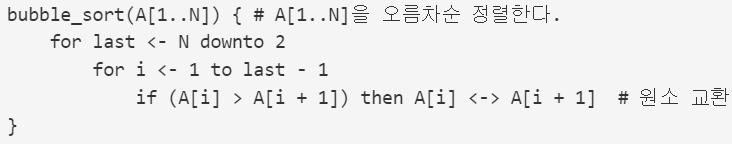
\includegraphics[width=0.8\textwidth]{Images/24074.png}
\end{problem}

\section{연습문제 C}
\begin{problem}
    (20084번) 숨겨진 길이 $N$의 바이너리 문자열 $T$가 있다. 여러분은 $S$가 $T$의 연속 부분문자열인지 판단하는 질의를 $t$번 이내로 사용하여 $T$를 알아내어야 한다.
    \begin{itemize}
        \item (서브테스크 1) $N \leq 5$, $t = 31$
        \item (서브테스크 2) $N \leq 100$, $t = 256$
        \item (서브테스크 3) $N \leq 1000$, $t = 1024$
    \end{itemize}
\end{problem}


\chapter{매개변수 탐색}
매개변수 탐색(parametric search)는 최적해 문제(optimal problem)을 풀기 위한 강력한 도구로 이분 탐색을 이용해 최적해를 찾는 방법이다. 기본적으로 답을 탐색한다는 아이디어를 기반으로 하며, $O(\log X)$의 시간복잡도를 곱해 최적해 문제를 결정 문제(decision problem)으로 바꿀 수 있는 방법이다. 이번 장에서는 앞 장에서 배운 이분 탐색을 바탕으로 매개변수 탐색을 하는 방법을 배운다.

\section{답을 탐색한다는 아이디어}
이분 탐색이 어떤 값 $x$가 정렬된 배열에 있는지 빠르게 탐색하는 방법이었다. 이 과정에서 $x$와 \texttt{arr[mid]}를 비교하였다. 이를 일반적으로 확장한다면 어떤 조건 $f(x)$에 대해

\begin{itemize}
    \item $f(mid)$가 참일 때 답이 $mid$ 이상이고,
    \item $f(mid)$가 거짓일 때 답이 $mid$ 미만이면
\end{itemize}

항상 이분 탐색의 원리를 적용할 수 있다. 이러한 관찰에 착안하여 답을 탐색하겠다는 아이디어가 매개변수 탐색이다. 구체적인 내용은 아래 Observation을 참고하자.

\begin{obs}
    조건 $f(x)$를 '답이 $x$인 경우가 존재하는가?'로 잡자. 그러면 다음 조건을 만족할 때 답에 대한 이분탐색을 통해 최적해를 찾아낼 수 있다. 구체적인 부등식 조건은 가능한 값의 범위만 배수로 짧아짐이 보장되면 어떤 것이던 상관없다.

    \begin{itemize}
        \item 답이 $mid$인 경우가 존재할 때 최적해가 $mid$ 이상이고,
        \item 답이 $mid$인 경우가 존재하지 않을 때 최적해가 $mid$ 미만이면
    \end{itemize}
\end{obs}

이러한 방식을 매개변수 탐색이라고 한다. 매개변수 탐색을 시행하면 최적해를 찾는 문제를 답이 $x$일 수 있는지 판단하는 문제로 바뀐다. 이와 관련된 자세한 내용은 6.2절을 참고하라.

이제 예시 문제를 통해 구현 방법을 알아보자.

\begin{example} \label{ex: parametric-search}
    자연수로만 이루어진 어떤 배열 $A$가 주어질 때, $A_i$ 중 $x$보다 큰 수의 개수가 $k$개 이하가 되는 $x$의 최솟값을 구하여라.
\end{example}

물론 \Cref{ex: parametric-search}은 일반적인 이분 탐색을 통해서도 풀 수 있을 것이다. 하지만 연습을 위해 매개변수 탐색을 통해 풀어보자. 먼저 매개변수 탐색의 조건을 만족하는지 확인해야 한다. $x=mid$일 때 조건을 만족하면 답은 $mid$ 이하이다. 또한 $x=mid$일 때 조건을 만족하지 않는다면 답은 $mid$ 초과이다. 따라서 조건을 만족함을 확인할 수 있다. 그리고 이 부등식 조건을 그대로 코드에 구현하면 된다. \Cref{code: parametric-search}은 이를 바탕으로 구현한 코드이다. \Cref{code: parametric-search}에서 \texttt{isAnswer(x)}는 $x$가 답이 될 수 있는지 확인하는 함수이다.

\begin{code} \label{code: parametric-search}
\Cref{ex: parametric-search}의 정답 코드
\begin{lstlisting}
#include <bits/stdc++.h>
using namespace std;

int n, arr[101010], k;
const int X = 1e9;

bool isAnswer(int x) {
    int cnt = 0;
    for (int i = 1; i <= n; i++) if (arr[i] > x) cnt++;
    return cnt <= k;
}

int main() {
    cin >> n;
    for (int i = 1; i <= n; i++) cin >> arr[i];

    cin >> k;
    int st = 0, ed = X;
    while (st < ed) {
        int mid = (st + ed) / 2;
        if (isAnswer(mid)) ed = mid;
        else st = mid + 1;
    }

    cout << st << "\n";

    return 0;
}
\end{lstlisting}
\end{code}

\texttt{X}를 $A_i$의 범위라 하면 가능한 답은 $1$과 $X$ 사이이므로 \texttt{isAnswer} 함수가 호출되는 횟수는 $O(\log X)$번이고 전체 시간복잡도는 $O(N \log X)$가 된다.

\section{결정 문제와 최적해 문제}
PS의 문제는 크게 \textbf{결정 문제(decision problem)}와 \textbf{최적해 문제(optimal problem)}로 나눌 수 있다. 결정 문제는 어떤 조건을 만족하는 해가 존재하는지 판별하고 그 해를 출력하는 문제를 말하고, 최적해 문제는 어떤 조건을 만족하는 해들 중 가장 원하는 값이 큰 해를 찾아 출력하는 문제이다. 자명하게도 최적해 문제는 결정 문제보다 어렵다.

그렇다면 최적해 문제를 결정 문제로 환원할 수 있을까? 만약 어떤 최적해 문제의 답이 $k$ 이하일 때 항상 가능함이 보장된다면, $1$부터 차례대로 가능한지 확인해보면 되므로 결정 문제로 바꿀 수 있다. 즉, $k$번 결정 문제를 해결하여 최적해 문제의 답을 구할 수 있다.

위 방식을 개선시키기 위해 명제 $p_i$를 "답이 $i$일 때 가능하다"라고 정의해보자. 그러면 $i \leq k$이면 $p_i$는 참이고, $i > k$이면 $p_i$는 거짓이다. 즉, 우리가 $p_i$를 나열한 배열을 생각한다면 앞쪽은 전부 참이고, 뒤쪽은 전부 거짓이므로 \textbf{정렬된 배열}로 볼 수 있다(참인 경우 $1$을 적고, 거짓인 경우 $0$을 적는다고 생각하면 편하다).

따라서 이 배열 $p_i$에 이분 탐색을 적용할 수 있고, 이것이 매개변수 탐색이다. 즉, 배열의 크기를 $X$라고 하면 $O(\log X)$번의 결정 문제를 해결하여 최적화 문제의 답을 구할 수 있다. 또한 $X$는 가능한 답의 범위가 될 것이다.

매개변수 탐색은 $O(\log X)$의 시간을 곱해 최적해 문제를 결정 문제로 만들어주는 강력한 도구이다. 물론 $p_i$ 배열이 정렬된 상태, 즉 어떤 값을 기준으로 명제의 참/거짓이 뒤집혀야 한다.

\section{연습문제 A}
\begin{problem}
    \Cref{ex: parametric-search}을 이분 탐색으로 풀어라.
\end{problem}

\begin{problem}
    $N$개의 정수 $A_i$가 주어진다. 다음 값이 $K$ 이상이 되는 가장 큰 자연수 $x$를 출력하라. $N \leq 10^6$, $1 \leq A_i \leq 10^9$이다.
    $$\sum_{i=1}^N {\max(A_i - x, 0)}$$
\end{problem}

\begin{problem}
    $N$개의 정수 $A_i$가 주어진다. 다음 값이 $K$ 이상이 되는 가장 작은 자연수 $t$를 출력하라. $N \leq 10^6$, $1 \leq A_i \leq 10^9$이다.
    $$\sum_{i=1}^N {\left\lfloor{\frac{t}{A_i}}\right\rfloor}$$
\end{problem}

\section{연습문제 B}

\begin{problem}
    (1166번) 한 변의 길이가 $A$인 정육면체 $N$개를 각 변이 평행하도록 $L \times W \times H$ 크기의 직육면체 박스에 모두 넣으려고 한다. 가능한 $N, L, W, H$가 주어질 때 가능한 $A$의 최댓값을 구하여라. 절대 및 상대 오차는 $10^{-9}$까지 허용한다. $N, L, W, H$는 모두 $10^9$ 이하의 자연수이다.
\end{problem}

\begin{problem}
    (3090번) 정수 $N$개로 이루어진 수열 $A_i$에서 수열의 한 수를 골라 $1$만큼 감소시키는 연산을 $t$번 이내로 수행하여 인접한 수의 차이의 최댓값의 최솟값을 출력하라. 다른 말로,
    $$\max_{1 \leq i < N} {\left\vert{A_{i+1}-A_i}\right\vert}$$
    의 최솟값을 출력하라. $N \leq 10^5$, $t \leq 10^9$, $A_i \leq 10^9$이다.
\end{problem}

\begin{problem}
    (10227번, IOI10) $1$부터 $RC$까지의 자연수가 정확히 한 번씩 적킨 $R \times C$ 크기의 격자에서 홀수 $H$와 $W$가 주어질 때 $H \times W$ 크기의 부분 격자에 속한 원소의 중앙값의 최솟값을 출력하라. $R \leq 3000$, $C \leq 3000$이다.
\end{problem}

\begin{problem}
    (11233번) 세 수 $a, b, c$가 주어질 때 정삼각형 내부의 점 중 세 꼭짓점으로부터의 거리가 $a, b, c$인 점이 존재할 수 있는 정삼각형의 넓이를 출력하라. 만약 그러한 정삼각형이 없다면 $-1$을 출력하면 된다. \textbf{고정 소숫점 방식으로 소숫점 셋째 자리까지 출력해야 한다}. $a, b, c$는 모두 $100$ 이하의 양의 실수이다.
\end{problem}

\begin{problem}
    (15470번*) 중심이 같고 반지름이 다른 두 원이 있고, 반지름이 더 작은 원 위의 점 $N$개가 있다. 이 점들을 변이 교차하지 않도록 이은 다각형의 각 변의 길이 $l_i$와 반지름이 더 큰 원의 원주 길이 $c$가 주어질 때 바깥 원과 다각형 사이의 면적을 출력하라. $N \leq 10$, $10 \leq c \leq 1000$이다.
\end{problem}

\begin{problem}
    (18543번*) 두 명의 플레이어가 다음 규칙으로 게임을 한다.
    \begin{itemize}
        \item 선 플레이어가 처음 선택권을 갖는다.
        \item 선택권을 가진 플레이어가 $1$부터 $m$ 사이의 정수 중 하나를 뽑는다. 각 정수가 나올 확률은 모두 같다.
        \item 수를 뽑은 플레이어는 이 수를 상대에게 넘기고 자신의 선택권을 유지할지, 아니면 자신이 이 수를 갖고 상대에게 선택권을 넘길지 선택한다.
    \end{itemize}
    두 플레이어가 모두 최적으로 플레이할 때, $n$번의 숫자를 가진 이후 선 플레이어와 후 플레이어의 숫자 합 차이의 기댓값을 $d_n$이라 하자. 그러면 $m \geq 3$에서 $\lim_{n \rightarrow \infty} d_n$의 값이 유리수로 존재함이 보장된다. 여러분은 $m$이 주어질 때마다 $\lim_{n \rightarrow \infty} d_n$의 값을 $\textrm{mod}~10^9+7$에 대한 표현으로 출력해야 한다. $3 \leq m \leq 10^9$이고 $m$이 주어지는 횟수 $t$는 $5 \times 10^5$회 이하이다.
\end{problem}

\begin{problem}
    (20106번*, IOI13) $0$번부터 $N-1$번까지의 번호가 붙여져 있는 일렬로 나열된 $N$개의 문과 $N$개의 스위치가 있다. 각 스위치는 어느 문에 연결되어 있는 스위치인지 모른다. 또 스위치를 켰을 때 문이 열려야 정상이지만, 일부 스위치의 경우에는 켰을 때 문이 닫히는 오류가 있다. 여러분은 최대 $70000$번 스위치를 조정한 후 처음으로 닫힌 문이 몇 번 문인지 확인할 수 있다. 이 결과를 토대로 $i$번쨰 스위치가 문이 열리기 위해 켜져야 하는지(1) 꺼져야 하는지(0) 출력하고 $i$번 스위치와 연결된 문의 번호도 출력해야 한다.
    \begin{itemize}
        \item (서브테스크 1) $N \leq 5000$, $i$번 스위치는 $i$번 문과 연결되어 있다.
        \item (서브테스크 2) $N \leq 5000$, 모든 스위치는 꺼졌을 때 문이 열린다.
        \item (서브테스크 3) $N \leq 100$
        \item (서브테스크 4) $N \leq 2000$
        \item (서브테스크 5) $N \leq 5000$
    \end{itemize}
\end{problem}

\begin{problem}
    (23791번) 길이 $N$의 두 배열 $A$와 $B$가 주어질 때, 다음 쿼리 $Q$개를 처리하는 프로그램을 작성하라. $N \leq 10^5$, $Q \leq 10^5$이고 $1 \leq A_i \leq 2^{31}-1$, $1 \leq B_i \leq 2^{31}-1$이다.
    \begin{itemize}
        \item $i, j, k$를 입력받아 $A_1$부터 $A_i$, 그리고 $B_1$부터 $B_j$ 까지의 숫자들 중 $k$번째로 작은 수를 출력하라. 다른 말로 $A_1$부터 $A_i$, 그리고 $B_1$부터 $B_j$ 까지의 숫자들 중에서 $x$ 이하인 수의 개수가 $k$인 가장 작은 $x$를 출력하라.
    \end{itemize}
\end{problem}

\begin{problem}
    (23107번*) 주어진 길이 $N$의 수열 $a_i, b_i, c_i$에 대해 다음 조건을 만족하는 순서쌍 $S=(s_0, s_1, \cdots, s_r)$을 모두 생각하자.
    \begin{itemize}
        \item $r$은 자연수
        \item $s_0 = 0, s_r = N$
        \item $s_i < s_{i+1}$ $(0 \leq i < r)$
    \end{itemize}
    $f(S)$를 다음과 같이 정의할 때 가능한 모든 $S$에 대해 $f(S)$의 최댓값을 출력하라. $N \leq 2 \cdot 10^5$이고 $a_i, b_i, c_i$는 절댓값이 $10^9$ 이하인 정수이다.
    $$f(S) = \min_{0 \leq i < r} {\left \{ b_{s_i} + c_{s_{i+1} - 1} + \sum_{s_i \leq j < s_{i+1}} {a_j} \right \}}$$
\end{problem}

\begin{problem}
    (27811번*) 양쪽 더미에 $L$개와 $R$개의 돌이 있다. $i$번째 라운드에 더 많은 개수의 돌이 있는 더미에서 $i$개의 돌을 가져간다. 만약 돌의 개수가 같으면 왼쪽 더미에서 $i$개의 돌을 가져간다. 만약 $i$번쨰 라운드에 양쪽 더미 모두에 있는 돌의 개수가 $i$개 미만이 되면 돌을 가져가지 못하므로 $i$번째 라운드가 진행되지 못하고 게임이 종료된다. 진행된 라운드의 숫자와, 게임 종료 후 양쪽 더미에 남은 돌의 개수를 출력하라. $T$번 $L$과 $R$이 주어졌을 때 출력해야 한다. $T \leq 1000$, $L \leq 10^{18}$, $R \leq 10^{18}$이다.
\end{problem}

\section{연습문제 C}
\begin{problem}
    (1557번) $1$이 아닌 제곱수로 나누어지지 않는 자연수를 크기 순으로 나열할 때 $K$번째로 나타나는 수를 출력하라. $K \leq 10^9$이다.
\end{problem}

\begin{problem}
    (2814번) 소수 $p$에 대해 가장 작은 소인수가 $p$인 자연수를 크기 순으로 나열할 때 $N$번째로 나타나는 수를 출력하라. $N \leq 10^9$, $p \leq 10^9$이다.
\end{problem}

\begin{problem}
    (5563번) 주어진 $N$개의 점을 두 그룹으로 분할하려고 한다. 각 그룹에는 한 개 이상의 점이 포함되어야 한다. 같은 그룹에 속하는 임의의 두 점 사이의 거리의 최댓값의 최솟값을 출력하라. 두 점 $(x_1, y_1)$과 $(x_2, y_2)$ 사이의 거리는 $|x_1 - x_2| + |y_1 - y_2|$로 계산된다. $3 \leq N \leq 10^5$이고 점의 $x$좌표와 $y$좌표는 절댓값이 $10^5$ 이하인 정수이다.
\end{problem}

\begin{problem}
    (9014번) 주어진 $N$개의 점을 두 개의 기준점 $(a_1, b_1)$과 $(a_2, b_2)$ 중 적어도 하나와 연결하려고 한다. 그런데 각각의 기준점은 적어도 $K$개의 점과 연결되어야 한다. 여러분은 $N$개의 점과 기준점과의 거리의 최댓값을 최소화해야 한다. 가능한 최솟값을 소숫점 첫째 자리에서 반올림한 값을 출력하라. 두 점 $(x_1, y_1)$과 $(x_2, y_2)$ 사이의 거리는 $|x_1 - x_2| + |y_1 - y_2|$로 계산된다. $2 \leq N \leq 10^5$, $K \leq N/2$이고 점의 $x$좌표와 $y$좌표는 절댓값이 $10^5$ 이하인 짝수이다.
\end{problem}

\begin{problem}
    (16655번) $N$명의 사람이 $S$달러를 나누어 가지려고 한다. 하지만 $N$명의 사람 각각이 요구하는 금액 $a_i$의 합이 $S$보다 커 문제가 되고 있다. 다음과 같이 \textit{공정한 분할}과 \textit{올바른 분할}을 정의할 때 \textit{공정한 분할}의 결과를 출력하라. $N \leq 5000$, $a_i \leq 5000$, $S \leq \sum_{i=1}^N {a_i}$이다.
    \begin{itemize}
        \item \textit{공정한 분할}은 합이 $S$인 수열 $c_i$들 중 모든 $(i, j)$ 쌍에 대해 $(a_i, a_j)$에 대한 합 $c_i + c_j$의 \textit{올바른 분할}이 $(c_i, c_j)$인 수열이다.
        \item $(x, y)$에 대한 합 $z$의 \textit{올바른 분할}은 $x+y \geq z$인 경우에 아래와 같이 정의된다.
        $$\begin{cases} 
            (\frac{z}{2}, \frac{z}{2}) & x \geq z, y \geq z \\
            (\frac{x}{2}, z - \frac{x}{2}) & x \leq z \leq y \\
            (z - \frac{y}{2}, \frac{y}{2}) & y \leq z \leq x \\
            (\frac{x+z-y}{2}, \frac{y+z-x}{2}) & x \leq z, y \leq z
        \end{cases}$$
    \end{itemize}
\end{problem}

\begin{problem}
    (18592번**) 중심이 $(x_i, y_i, z_i)$이고 반지름이 $r_i$인 $N$개의 구를 생각하자. $N(N-1)/2$개의 $(i, j)$ 쌍에 대하여 $d(i, j)$를 두 구 사이의 최단거리로 정의하자(겹치면 $0$이다). 수식으로는 아래와 같이 나타낼 수 있다.
    $$d(i, j) = \max \left( 0, \sqrt{(x_i - x_j)^2 + (y_i - y_j)^2 + (z_i - z_j)^2} - r_i - r_j \right)$$
    모든 $(i, j)$ 쌍에 대한 $\lceil d(i, j) \rceil$를 크기 순으로 나열할 때 가장 작은 $k$개를 증가하는 순서로 출력하라. $N \leq 10^5$, $k \leq 300$, $0 \leq x_i, y_i, z_i\leq 10^6$, $1 \leq r_i \leq 10^6$이다.
\end{problem}

\begin{problem}
    (26610번) $N$개의 돌이 있는 더미에서 $i$번째 턴에 $1 \leq k \leq T$인 자연수 $k$에 대해 $(X+i) \times k$개의 돌을 가져가야 하는 게임을 생각하자. 만약 더 이상 조건을 만족하게 돌을 가져갈 수 없으면 게임이 종료된다. 여러분은 다음 쿼리 $Q$개에 대해 답해야 한다. $Q \leq 3 \times 10^5$, $1 \leq X < N \leq 5 \times 10^8$, $2 \leq T \leq 10^8$이다.
    \begin{itemize}
        \item 이 게임이 종료되었을 때 가장 적은 개수의 돌을 남겨야 하고 만약 그러한 방법이 여러 개라면 가장 빠르게 게임을 끝내야 한다. 최적의 방식으로 플레이했을 때 돌을 가져가는 횟수를 출력하라.
    \end{itemize}
\end{problem}

\chapter{병렬 이분 탐색}
병렬 이분 탐색(parallel binary search)은 매개변수 탐색 과정을 여러 번 처리해야 할 때 빠르게 처리하기 위한 방법이다. 기본적으로 매개변수 탐색을 여러 번 처리할 때 같은 값 $x$에 대해 $x$가 답이 될 수 있는지 판단하는 것이 중복적으로 나타나고, 이 시간을 줄이겠다는 아이디어에서 만들어진 알고리즘이다. 이번 장에서는 6장에서 배운 매개변수 탐색을 바탕으로 병렬 이분 탐색을 하는 방법을 배운다.

\textbf{* 주의: 병렬 이분 탐색은 뒤쪽 챕터의 알고리즘과 함께 쓰이는 경우가 전부이므로, 뒤의 내용을 공부하다가 필요한 시점에 다시 보는 것을 추천한다.}

\section{쿼리와 이분 탐색}
\Cref{ex: parametric-search}에 쿼리를 추가한 문제를 생각하자.
\begin{example} \label{ex: parallel-binary-search}
    자연수로만 이루어진 어떤 배열 $A$가 주어질 때, 다음 쿼리 $Q$개를 처리하는 프로그램을 작성하라.
    \begin{itemize}
        \item 쿼리: $A_i$ 중 $x$보다 큰 수의 개수가 $k$개 이하가 되는 $x$의 최솟값을 구하여라.
    \end{itemize}
\end{example}

만약 매개변수 탐색을 $Q$번 진행한다면 시간복잡도가 $O(NQ\log X)$가 될 것이다. 하지만, 병렬 이분 탐색을 사용할 경우 $O(N \log Q \log X + Q \log X)$로 줄일 수 있다.

각 쿼리의 $k$를 $q_i$라고 놓자. 그리고 각 쿼리마다 현재 가능한 값의 범위 $[s_i, e_i]$를 생각하자. 초깃값은 모든 $i$에서 $s_i=1, e_i=X$일 것이다. 이제 $x=m = (s+e)/2$에서 $x$보다 큰 수의 개수를 세자. 이 개수보다 $q_i$가 큰 쿼리는 $s_i$가 바뀌고, $q_i$가 그 개수 이하인 쿼리는 $e_i$가 바뀔 것이다.

이제 각 $[s_i, e_i]$가 절반으로 감소하였다. 이와 동시에 가능한 $x=m$의 값은 두 가지가 되었다. 만약 이 두 가지 $x=m$에 대해 각각 $O(N)$의 시간으로 $x$보다 큰 수의 개수를 계산한다면 시간복잡도의 개선이 전혀 일어나지 않을 것이다(\Cref{pb: wrong-pbs-time}). 병렬 이분 탐색을 통해 시간복잡도를 개선하려면 \textbf{한 번의 탐색으로 다양한 $x$ 값에 대해 원하는 값(여기서는 $x$보다 큰 수)}을 구할 수 있어야 한다.

이를 위해 이분탐색을 사용할 수 있다. 가능한 각 쿼리에서 $m$의 값을 $x_1, x_2, \cdots, x_q$라고 놓고 이를 정렬하자. 그리고 배열 $c_i$에 값이 $x_{i-1}$ 초과 $x_i$ 이하인 수의 개수를 저장하자(편의상 $x_0=0$, $x_{q+1}=X$로 놓는다). 이 과정은 $A_i$ 초과인 가장 앞에 있는 수 $x_j$를 배열 $x$에서 이분탐색을 통해 찾으면, $(x_{j-1}, x_j]$에 $A_i$가 존재하므로 $c_j$를 $1$ 증가시키면 된다. 따라서 $O(N \log Q)$의 시간에 $c_i$를 계산할 수 있다. 또한 $c_i$의 정의에 의해 $i+1$부터 $q+1$까지의 $c_i$의 부분 합이 각 $x_i$보다 큰 수의 개수이므로 각 $x_q$에 대한 답을 $O(Q)$의 시간에 찾을 수 있다. 구현은 다음 \Cref{code: parallel-binary-search}을 참고하라.

\begin{code} \label{code: parallel-binary-search}
\Cref{ex: parallel-binary-search}의 정답 코드
\begin{lstlisting}
#include <bits/stdc++.h>
using namespace std;

int n, arr[101010], q, k[101010];
int s[101010], e[101010], c[101010], sum[101010];
const int X = (1<<30);

int main() {
    cin >> n;
    for (int i = 1; i <= n; i++) cin >> arr[i];
    cin >> q;
    for (int i = 1; i <= q; i++) cin >> k[i];

    for (int i = 1; i <= q; i++) {
        s[i] = 1;
        e[i] = X;
    }
    while (s[1] < e[1]) {
        for (int i = 1; i <= q + 1; i++) c[i] = sum[i] = 0;
        vector< pair<int, int> > m;
        m.push_back({0, 0});
        for (int i = 1; i <= q; i++) m.push_back({(s[i] + e[i]) / 2, i});
        m.push_back({X, q + 1});
        sort(m.begin(), m.end());

        for (int i = 1; i <= n; i++) {
            int j = lower_bound(m.begin(), m.end(), make_pair(arr[i] + 1, 0)) - m.begin();
            c[j]++;
        }

        for (int i = 1; i <= q + 1; i++) sum[i] = sum[i - 1] + c[i];
        for (int i = 1; i <= q; i++) {
            if (sum[q + 1] - sum[i] <= k[m[i].second]) e[m[i].second] = m[i].first;
            else s[m[i].second] = m[i].first + 1;
        }
    }

    for (int i = 1; i <= q; i++) cout << s[i] << " ";

    return 0;
}
\end{lstlisting}
\end{code}

정리하면 병렬 이분 탐색은 최적해 문제 쿼리를 업데이트 쿼리와 결정 문제 쿼리로 환원하는 것이다:
\begin{itemize}
    \item 업데이트 쿼리: 결정 문제의 고정된 기준값 $m$이 증가할 때, 결정 문제를 빠르게 해결하기 위해 저장해야 하는 값들을 갱신
    \item 결정 문제 쿼리: 주어진 $m$에 대해 결정 문제를 해결
\end{itemize}

이처럼 업데이트 쿼리가 추가되기 때문에 업데이트가 있는 상황에서 주어진 문제를 빠르게 해결하기 위해 사용되는 자료구조들과 함께 쓰이는 경우가 많다.

\section{연습문제 A}
\begin{problem} \label{pb: wrong-pbs-time}
    \Cref{ex: parallel-binary-search}에 대한 병렬 이분 탐색 과정에서 $Q$개의 쿼리에서 나온 모든 $m$에 대해 $O(N)$의 시간으로 탐색한다면 시간복잡도가 어떻게 되는가?
\end{problem}
\begin{problem}
    \Cref{code: parallel-binary-search}에서 $X$를 \texttt{1<<30}으로 놓은 이유가 무엇인가?
\end{problem}
\begin{problem}
    \Cref{code: parallel-binary-search}에서 부분 합을 구간 $[i+1, q+1]$로 처리한 이유가 무엇인가? 왜 $[i+1, q]$가 아닌가?
\end{problem}
\begin{problem}
    사실 \Cref{ex: parallel-binary-search}은 병렬 이분 탐색 없이 해결할 수 있다. 병렬 이분 탐색 없이 해결하는 코드를 짜고, 그 코드의 시간복잡도를 구하라.
\end{problem}

\section{연습문제 B}

\begin{problem}
    $x_i$가 $x_{i-1} \cdot a + b$를 $10^9+7$로 나눈 나머지인 점화관계를 가진 길이 $N$의 수열 $x_i$에 대해 $x_i$에서 $q$번째로 작은 원소를 찾는 쿼리 $Q$개를 처리하는 프로그램을 작성하라. 정확히 말하면 $y$보다 작은 $x_i$의 원소의 개수가 $q$인 가장 작은 $y$를 찾아야 한다. \textbf{단, $x_i$를 모두 저장할만큼 메모리가 충분하지 않다.}
    \begin{itemize}
        \item (12926번) $N \leq 10^6$, $Q \leq 100$, $x_0, a, b$는 $10^9+7$ 미만의 음 아닌 정수
        \item (12921번) $N \leq 2 \cdot 10^6$, $Q \leq 1000$, $x_0, a, b$는 $10^9+7$ 미만의 음 아닌 정수
    \end{itemize}
\end{problem}

\section{연습문제 C}
\textbf{* 주의: 본 챕터의 연습문제 C는 뒤에 나오는 자료구조를 알아야 풀 수 있는 문제로 구성되어 있다.} 만약, 이 책을 처음부터 읽고 있으며 뒤의 자료구조에 관한 지식이 없다면 연습문제 C를 보며 아이디어만 생각하거나 나중에 다시 풀어보자.

\begin{problem}
    (8217번) 원이 $M$ 분할되어 각각 $1$번부터 $M$번까지 번호가 붙어 있다. 특히, $1$번과 $M$번은 붙어 있다. 그리고 각각은 $N$명의 사람 중 한 명이 소유하고 있으며 이 정보는 입력으로 주어진다. 또한 $Q$일 동안 연속된 부채꼴 $[l_i, r_i]$번에서 각각 $a_i$만큼의 석유가 나온다($1 \leq i \leq Q$). 참고로 $l_i > r_i$이면 $[l_i, r_i]$는 $[l_i, m] \cup [1, r_i]$를 뜻한다. 각 사람이 자신이 가진 땅의 석유를 매일 모을 때, 각 사람마다 원하는 목표치인 $p_j~(1 \leq j \leq N)$ 이상의 석유를 얻기 위해 기다려야 하는 날의 수를 출력하라. $N \leq 3 \times 10^5$, $M \leq 3 \times 10^5$, $Q \leq 3 \times 10^5$이고 $a_i \leq 10^9$, $p_i \leq 10^9$이다.
\end{problem}

\begin{problem}
    (9877번) $10^9$ 이하의 음 아닌 정수가 적힌 $N \times M$ 격자에서 정수 $T$가 주어질 때 각 셀에 대해 각 칸에 대해 다음 쿼리를 처리하라. $N \leq 500$, $M \leq 500$이다.
    \begin{itemize}
        \item 상하좌우로 인접한 칸 중 적힌 수의 차이가 $D$ 이하인 칸으로 이동하는 것만 허용할 때 시작 칸 $(a, b)$에서 도달할 수 있는 칸의 개수가 $T$개 이상이 되도록 $D$를 정하자. 가능한 $D$의 최솟값을 출력하라.
    \end{itemize}
\end{problem}

\begin{problem}
    (13952번) 방해물이 있는 $N \times N$ 격자에서 다음 쿼리 $Q$개를 처리하라. $N \leq 1000$, $Q \leq 3 \times 10^5$이다.
    \begin{itemize}
        \item $(x_a, y_a)$가 중심인 홀수 길이의 정사각형이 방해물에 걸리지 않고 상하좌우로 평행하게 이동하여 중심이 $(x_b, y_b)$인 위치까지 이동할 수 있는 정사각형 길이의 최댓값을 출력하라. 그 어떤 정사각형도 불가능하면 $0$을 출력하면 된다.
    \end{itemize}
\end{problem}

\begin{problem}
    (16976번) 컴퓨터를 한 대 갖고 있는 $N$명의 사람이 $M$종류의 게임 중 하나의 게임을 구매했다. 그리고 순차적으로 $Q$번 두 사람이 가진 컴퓨터 사이에 랜선을 연결할 것이다. $i$번 게임을 구매한 모든 사람의 컴퓨터가 연결되었을 때 $i$번 게임을 시작할 때, 각 게임이 몇 개의 랜선을 연결한 이후에 시작될 수 있는지 출력하라. $N \leq 10^5$, $M \leq 10^5$, $Q \leq 10^5$이다.
\end{problem}

\begin{problem}
    (20654번) $N$개의 액체가 있고, 각 액체는 맛 $d_i$와 단위용량당 가격 $p_i$가 정해져 있다. 이 액체 중 몇 개를 원하는 양만큼 넣어 음료를 만들고 싶다. 단, $i$번 액체는 $l_i$ 이하만큼 넣어야 한다. 이때 다음 쿼리 $M$개를 처리하는 프로그램을 작성하라. $N \leq 10^5$, $M \leq 10^5$이고 $d_i, p_i, l_i$는 $10^5$ 이하의 자연수, $g_i, L_i$는 $10^{18}$ 이하의 자연수이다.
    \begin{itemize}
        \item 음료를 만드는데 필요한 액체의 가격이 $g_j$ 이하이며 음료의 용량이 $L_j$ 이상인 음료 중에서 음료에 포함되는 액체의 맛 $d_i$의 최솟값의 가능한 최댓값을 출력하라.
    \end{itemize}
\end{problem}

\begin{problem}
    (21095번*) 길이 $N$의 수열 $A_i$가 주어질 때, 다음 쿼리 $Q$개를 처리하는 프로그램을 작성하라.
    \begin{itemize}
        \item $l, r, k$가 주어질 때 모든 $1 \leq i \leq k$에 대해 $C_i + C_{(i~\textrm{mod}~k)+1} \leq W$이면서 $A[l..r]$에서 몇 개의 수를 지워 $k$개의 수를 남긴 부분 수열인 $C_i$가 존재하는 $W$의 최솟값을 출력하라.
    \end{itemize}
\end{problem}

\begin{problem}
    (25458번*) \url{https://www.acmicpc.net/problem/25458}
\end{problem}

\begin{problem}
    (27199번*) 주어진 홀수 길이의 배열에서 \textbf{연속된 세 숫자 중 중앙값만 남기는 연산}을 배열의 길이가 $1$이 될 때까지 해 남길 수 있는 수의 최댓값을 배열의 \textit{중앙값 평균}이라고 하자. 길이 $N$의 배열 $A_i$와 $Q$개의 $(l, r)$ 쌍이 주어질 때 $A[l..r]$의 \textit{중앙값 평균}을 출력하는 프로그램을 작성하라. $N \leq 50000$, $Q \leq 10^5$, $0 \leq A_i \leq 10^9$이고 모든 쿼리에서 $r-l+1$은 홀수이다.
\end{problem}

\chapter{투 포인터}
투 포인터(Two pointer)는 한 배열의 어떤 부분 구간에 대한 문제를 풀 때, 두 개의 포인터를 사용하여 전체 구간을 탐색하지 않고 빠르게 문제를 해결하는 방식이다. 보통 제일 앞에 두 개의 포인터 \texttt{p}와 \texttt{q}를 잡고 두 포인터를 오른쪽으로 이동시키며 문제를 해결한다. 이 장에서는 투 포인터로 해결할 수 있는 문제가 무엇이고 어떻게 해결하는지 다룬다.

\section{가능한 구간을 찾는 문제}
다음과 같은 문제를 생각하자.

\begin{example} \label{ex: two-pointer}
    (15565번) $0$ 또는 $1$로만 이루어진 길이 $N$의 이진 배열에서 $1$의 개수가 $k$개 이상인 구간들 중 가장 짧은 구간의 길이를 출력하라.
\end{example}

만약 가능한 $O(N^2)$개의 모든 구간을 고려한다면 부분 합을 사용할 때 각 구간이 조건을 만족함을 $O(1)$에 확인할 수 있으므로 시간복잡도가 $O(N^2)$이 된다. 하지만 투 포인터 알고리즘을 사용하면 $O(N)$으로 줄일 수 있다.

이를 위해 해야 하는 중요한 관찰 두 가지가 있다.
\begin{obs}
    다음이 성립한다.
    \begin{itemize}
        \item 구간 $[s, e]$가 조건을 만족한다면 $[s, e]$를 포함하는 구간은 확인 필요가 없다. $[s, e]$보다 길이가 길기 때문이다.
        \item 구간 $[s, e]$가 조건을 만족하지 않는다면 $[s, e]$에 포함되는 구간은 확인할 필요가 없다. 자명히 $1$의 개수가 $k$개보다 작기 때문이다.
    \end{itemize}
\end{obs}
이제 고정된 $s$에 대해 살펴봐야 할 $e$의 범위를 생각해보자. 기본적으로 $e$는 증가한다고 가정한다. 만약 $[s, e]$가 조건을 만족한다면 $i>e$인 $[s, i]$는 살펴볼 필요가 없다. 따라서 $s$를 $s+1$로 증가시키자. 반대로 $[s, e]$가 조건을 만족하지 않는다면 $i<e$인 $[s, i]$는 살펴볼 필요가 없다. 따라서 $e$를 $e+1$로 증가시키자. 이렇게 되면 각 과정에서 $s$가 $1$ 증가하거나 $e$가 $1$ 증가하므로 최대 $2N$번 반복되며, $O(N)$의 시간복잡도에 문제를 해결할 수 있게 된다. 구현은 \Cref{code: two-pointer}을 참고하라.

\begin{code} \label{code: two-pointer}
\Cref{ex: two-pointer}의 정답 코드
\begin{lstlisting}
#include <bits/stdc++.h>
using namespace std;

int n, arr[101010], k;
int sum[101010], ans;

int main() {
    cin >> n;
    for (int i = 1; i <= n; i++) cin >> arr[i];
    cin >> k;

    for (int i = 1; i <= n; i++) sum[i] = sum[i - 1] + arr[i];

    int s = 1, e = 1;
    ans = n;
    while (true) {
        if (e > n) break;
        if (sum[e] - sum[s - 1] >= k) {
            ans = min(ans, e - s + 1);
            s++;
        }
        else e++;
    }

    cout << ans << "\n";

    return 0;
}
\end{lstlisting}
\end{code}

투 포인터라는 이름은 $s$와 $e$를 인덱스가 아니라 배열의 $s$번째 값과 $e$번째 값을 가리키는 포인터로 생각하여 나온 이름이다. $s$와 $e$를 포인터로 생각할 수 있는 이유는 $s$와 $e$는 증가만 하고, 이러한 특징이 포인터가 증가해 다음 값을 가리키는 것과 비슷하기 때문이다.

\section{투 포인터가 사용될 조건}
그렇다면 투 포인터가 사용될 수 있는 조건은 무엇일까? 다시 위의 관찰로 돌아가보면 다음이 성립해야 함을 알 수 있다.
\begin{obs}
    구간 $[s, e]$를 평가하는 함수 $f(x)$와(값이 클수록 좋다고 가정) 구간 $[s, e]$가 조건을 만족하는지 여부를 리턴하는 함수 $g(x)$에 대해
    \begin{itemize}
        \item 어떤 구간 $[s, e]$의 $f(x)$보다 $[s, e]$를 포함하는 구간의 $f$ 값이 더 작고,
        \item 어떤 구간 $[s, e]$의 $g(x)$가 거짓이면 $[s, e]$에 포함되는 구간의 $g$ 값이 거짓이어야 한다.
    \end{itemize}
\end{obs}

\Cref{ex: two-pointer}은 $f(x) = -(e - s + 1)$(음의 부호는 작을수록 좋기 때문에 붙었음), $g(x)=(1\textrm{의 개수} \geq k)$인 상황으로 볼 수 있다.

마지막으로 임의의 투 포인터 문제의 시간복잡도를 논의해보자. 매 과정에서 $g([s, e])$가 성립하는지 확인하고, 전체 과정은 $2N$번 이하이므로 $g([s, e])$를 계산하는 시간복잡도가 $T(n)$이면 전체 시간복잡도는 $N \cdot T(N)$이다.

\section{연습문제 A}
\begin{problem}
    \Cref{ex: two-pointer}은 부분 합을 사용하지 않아도 문제를 해결할 수 있다. 부분 합을 사용하지 않고 \Cref{ex: two-pointer}을 해결하는 코드를 작성하라.
\end{problem}

\section{연습문제 B}

\begin{problem}
    (1806번) 길이가 $N$인 수열의 연속한 부분수열들 중 수열의 원소들의 합이 $S$ 이상인 가장 짧은 부분수열의 길이를 출력하라. $N \leq 10^5$, $S \leq 10^9$이고 각 수열의 원소는 $10000$ 이하의 자연수이다.
\end{problem}

\begin{problem}
    (2470번, KOI10) $N$개의 수가 주어질 때 두 개를 골라 합을 $0$에 가장 가깝게 만드려고 한다. 그때 고른 두 수를 \textbf{아무거나} 하나 출력한다. $N \leq 10^5$이고 각 수는 절댓값이 $10^9$ 이하인 정수이며 모두 다르다.
\end{problem}

\begin{problem}
    (2473번, KOI10) $N$개의 수가 주어질 때 세 개를 골라 합을 $0$에 가장 가깝게 만드려고 한다. 그때 고른 세 수를 \textbf{아무거나} 하나 출력한다. $N \leq 5000$이고 각 수는 절댓값이 $10^9$ 이하인 정수이며 모두 다르다.
\end{problem}

\begin{problem}
    (7453번) $N$개의 수가 주어질 때 네 개를 골라 합이 $0$이 되는 방법의 수를 출력하라. $N \leq 4000$이고 각 수는 절댓값이 $2^28$ 이하인 정수이다.
\end{problem}

\begin{problem}
    (13364번*) $N$개의 점을 순서대로 연결하여 그린 $N-1$개의 선분의 집합과 $M$개의 점을 순서대로 연결하여 그린 $M-1$개의 선분의 집합을 생각하자. 각각을 경로로 하여 두 물체가 이동한다. 즉, 첫 번째 물체는 첫 번째 점에서 $N$번째 점의 방향으로, 두 번째 물체는 첫 번쨰 점에서 $M$번째 점의 방향으로 이동한다. 두 물체가 같은 속도로 이동할 때 두 물체 사이의 거리가 가장 가까울 때 그 값을 출력하라. 단, 한 물체가 먼저 마지막 점에 도달하면 물체는 소멸한다고 가정한다. $N, M \leq 10^5$이고 각 점의 $x$좌표와 $y$좌표는 $10000$ 이하의 음 아닌 정수이다.
\end{problem}

\begin{problem}
    (16598번) 연속된 출석 일수가 길수록 좋은 보상을 주는 앱이 있다. 그런데 버그가 나서 추가로 $P$일이 출석으로 인정되는 문제가 생겼다! 이 앱에 출석한 $N$일의 날짜 $d_i$가 주어질 때, 가능한 연속 출석 일수의 최댓값을 출력하라. 즉, 적절히 출석으로 인정될 $P$일을 고를 때 가능한 최대 연속 출석 일수를 구하는 것이다. $N \leq 2 \cdot 10^5$, $P \leq 2 \cdot 10^5$, $0 \leq d_1 < d_2 < \cdots < d_n \leq 10^6$이다.
\end{problem}

\begin{problem}
    (20085번*, IOI16) 자연수로 이루어진 길이 $N$의 수열 $a_i$와 범위 $[l, r]$이 주어진다. 이때 길이 $N$의 수열에서 적절히 몇 개의 수를 골라 합이 $[l, r]$의 범위에 속하게 할 수 있는지 판단하고, 가능하다면 선택되는 수열의 수의 인덱스를 오름차순으로 출력하라. 단, $r - l \leq \max a_i - \min a_i$가 보장된다.
    \begin{itemize}
        \item (서브테스크 1) $n \leq 100$, $a_i \leq 100$, $1 \leq l \leq r \leq 1000$, $a_i$는 모든 $i$에서 같다.
        \item (서브테스크 2) $n \leq 100$, $a_i \leq 1000$, $1 \leq l \leq r \leq 1000$, $\max a_i - \min a_i \leq 1$
        \item (서브테스크 3) $n \leq 100$, $a_i \leq 1000$, $1 \leq l \leq r \leq 1000$
        \item (서브테스크 4) $n \leq 10000$, $a_i \leq 10000$, $1 \leq l \leq r \leq 10000$
        \item (서브테스크 5) $n \leq 10000$, $a_i \leq 5 \times 10^5$, $1 \leq l \leq r \leq 5 \times 10^5$
        \item (서브테스크 6) $n \leq 100$, $a_i < 2^31$, $1 \leq l \leq r < 2^31$
    \end{itemize}
\end{problem}

\begin{problem}
    (20133번*) $N$개의 점이 주어질 때 서로 다른 \textit{모래시계 모양}의 개수를 출력하라. $N \leq 1500$이고 점의 $x$좌표와 $y$좌표는 절댓값이 $10^9$ 이하인 정수이며 어떤 세 점도 한 직선을 이루지 않는다.
    \begin{itemize}
        \item \textit{모래시계 모양}은 두 삼각형이 한 점을 공유하고 두 삼각형이 겹치지 않는 모양이다.
        \item 서로 다른 \textit{모래시계 모양}이라는 것은 구성하는 점과 선분이 중 하나라도 다른 것이다.
    \end{itemize}
\end{problem}

\begin{problem}
    (20922번) 길이 $N$의 수열이 주어질 때, 구간에 포함된 임의의 정수가 구간에 $k$개 이하로 포함되는 가장 긴 연속 부분 수열의 길이를 출력하라. $N \leq 2 \cdot 10^5$, $1 \leq k \leq 100$이고 수열의 각 정수는 $100000$ 이하의 자연수이다.
\end{problem}

\begin{problem}
    (20985번*) $1$부터 $N$까지 번호가 매겨진 $N$개의 눈덩이가 있다. $i$번 눈덩이는 $x_i$에 있고 처음 무게는 0이다. 이 눈덩이는 바람에 의해 평원을 구르며 크기가 커지게 된다. 정확히는 다음과 같은 방식이다.
    \begin{itemize}
        \item $Q$일 동안 정수 $w$로 표현되는 바람이 분다. 이 바람이 불면 하루가 끝나고 나서 눈덩이가 $x_i$에서 $x_i + w$로 이동한다. 또한 모든 눈덩이는 동시에 이동한다.
        \item 구간 $[a, a+1]$에 눈이 있다면 그 구간을 지나간 눈덩이의 무게가 1 증가한다. 그리고 눈이 사라진다. 만약 눈이 없다면 무게의 변화는 없다.
    \end{itemize}
    $Q$일이 지난 이후 $N$개의 눈덩이의 무게를 각각 출력하라.
\end{problem}

\begin{problem}
    (25405번*, KOI22) 레벨이 $L_i$인 $N$명의 게임 캐릭터에 대해 다음과 같은 규칙의 트레이닝을 $M$번 진행하였을 때 모든 트레이닝이 끝난 이후 각 캐릭터들의 레벨을 오름차순으로 정렬하여 출력하라.
    \begin{itemize}
        \item 한 번의 트레이닝은 레벨이 낮은 순서대로 $K$개의 캐릭터를 고르고 선택된 캐릭터들의 레벨을 $1$ 올리는 것이다. 레벨이 같은 캐릭터가 여러 명인 경우에는 아무거나 고른다.
    \end{itemize}
    \begin{itemize}
        \item (서브테스크 1) $N \leq 1000$, $M \leq 1000$, $K \leq N$, $L_i \leq 10^9$
        \item (서브테스크 2) $N \leq 10^5$, $M \leq 10^9$, $K = 1$, $L_i \leq 10^9$
        \item (서브테스크 3) $N \leq 10^5$, $M \leq 10^5$, $K \leq N$, $L_i \leq 10^9$
        \item (서브테스크 4) $N \leq 10^5$, $M \leq 10^9$, $K \leq N$, $L_i \leq 10^9$
    \end{itemize}
\end{problem}

\begin{problem}
    (26829번*) $n$개의 참-거짓 질문에 대한 답변이 모두 다른 $m$명의 사람이 있다. 그들의 답변은 $[0, 2^n)$ 사이의 숫자로 표현되며, $i$번째 비트가 $1$이라는 것은 $i+1$번째 질문에 대해 참으로 답변했음을 의미한다. $m$명을 인덱스 기준으로 $[1, p]$와 $[p+1, m]$의 두 그룹으로 나눌 때 다음 조건을 만족하도록 나누는 경우의 수를 구하여라. $n \leq 30$, $m \leq \min(2^n, 2 \times 10^6)$이다.
    \begin{itemize}
        \item 모든 $1 \leq i \leq n$에 대해 $i$번 질문에 참이라 대답한 사람이 \textbf{두 그룹 모두 존재하거나 두 그룹 모두 존재하지 않아야 한다}.
        \item 모든 $1 \leq i \leq n$에 대해 $i$번 질문에 거짓이라 대답한 사람이 \textbf{두 그룹 모두 존재하거나 두 그룹 모두 존재하지 않아야 한다}.
    \end{itemize}
\end{problem}

\begin{problem}
    (27916번*) $N$개의 아파트가 수직선 상에 있고, 각 아파트의 위치는 $A_i$로 표현된다. 각 아파트는 정확히 하나의 아파트 단지에 속해야 하고, 아파트 단지는 최소 $M$개의 아파트를 포함하는 연속된 번호를 가진 아파트의 집합이어야 한다. 다른 말로 모든 아파트 단지는 $[L, R]$로 표현될 수 있고, 이렇게 표현된다면 아파트 단지의 크기는 $A_R - A_L$이다. 다음 쿼리 $Q$개를 해결하는 프로그램을 작성하라.
    \begin{itemize}
        \item 아파트 단지의 크기를 $X_i$ 이하로 할 수 있는 아파트 단지의 구성 방법이 존재한다면 \texttt{1}을, 존재하지 않는다면 \texttt{0}을 출력하라.
    \end{itemize}
    $1 \leq A_1 < A_2 < \cdots < A_N \leq 10^9$, $0 \leq X_i \leq 10^9$이고 서브테스크마다 추가 제약 조건이 있다.
    \begin{itemize}
        \item (서브테스크 1) $N \leq 3 \times 10^5$, $M = N$, $Q = 1$
        \item (서브테스크 2) $N \leq 1000$, $M \leq N$, $Q \leq 3 \times 10^5$
        \item (서브테스크 3) $N \leq 3 \times 10^5$, $M \leq N$, $Q = 1$
        \item (서브테스크 4) $N \leq 1000$, $M \leq N$, $Q \leq 3 \times 10^5$
        \item (서브테스크 5) $N \leq 3 \times 10^5$, $M \leq N$, $Q \leq 3 \times 10^5$
    \end{itemize}
\end{problem}

\begin{problem}
    (28081번) 영역 $[0, W] \times [0, H]$를 $y$축과 평행한 $M$개의 선 $x=x_i$과 $x$축과 평행한 $N$개의 선 $y=y_i$로 나누면 각각의 직사각형 영역이 만들어진다. 이 직사각형 영역들 중 넓이가 $K$ 이하인 영역의 개수를 출력하라. $2 \leq H, W \leq 10^9$, $N, M \leq 10^5$, $1 \leq x_1 < x_2 < \cdots < x_M < W$, $1 \leq y_1 < y_2 < \cdots < y_N < H$이다.
\end{problem}

\section{연습문제 C}
\begin{problem}
    (8191번) 길이 $N$의 수열 $A_i$가 주어질 때, $M$번 $k$가 주어질 때마다 다음 쿼리를 해결하는 프로그램을 작성하라. $N \leq 10^6$, $M \leq 50$, $A_i \leq 10^9$, $k \leq 10^9$이다.
    \begin{itemize}
        \item $A_i > k$인 한 $i$를 골라 $A_i$를 $1$ 줄이고 $i > 1$일 때 $A_{i-1}$을 $1$ 늘리거나 $i < N$일 때 $A_{i+1}$을 $1$ 늘리는 연산을 사용할 수 있다. 이 연산을 통해 $A_i \geq k$인 연속된 구간의 길이를 최대화시키고자 할 때 가능한 최댓값을 출력하라.
    \end{itemize}
\end{problem}

\begin{problem}
    (10010번) $N$개의 도시가 있고 일부 도시 쌍이 양방향 도로로 연결되어 있아. 구체적으로 $1 \leq i < N$에 대해 $0$번 도시와 $i$번 도시가 연결되어 있고, $1 \leq i < N-1$에 대해 $i$번 도시와 $i+1$번 도시가 연결되어 있고, 마지막으로 $N-1$번 도시와 $1$번 도시가 연결되어 있다. 앞에서 설명한 순서대로 각 도로를 이동하는데 걸리는 시간이 주어질 때, 최단거리가 가장 먼 두 도시 사이의 거리를 출력하라. $N \leq 5 \times 10^5$이고 각 도로를 이동하는데 걸리는 시간은 양의 정수이며, 임의의 두 도시 사이의 최단거리는 $10^9$ 이하이다.
\end{problem}

\begin{problem}
    (10132번) 원형 철길 상의 $N$개의 기차역이 있다. $1 \leq i < N$에 대해 $i$번쨰 지점과 $i+1$번쨰 사이의 거리는 $l_i$, $N$번째 지점과 첫 번째 지점 사이의 거리는 $l_N$이다. 또한, 이 곳에서는 총 $s$대의 기차가 사용된다. 다음은 이 철도 체계에 대한 설명이다.
    \begin{itemize}
        \item $i$번째 기차는 연료를 꽉 치우고 $d_i$만큼 이동할 수 있다. 
        \item 연료는 역에서만 채울 수 있으므로 각 기차는 다음 역에 도달할만큼 충분히 연료가 남아있지 않다면 연료를 채워야 한다. 물론 그 양이 충분하더라도 원하면 연료를 채울 수 있다. 
        \item 각 $s$대의 기차가 하루에 딱 한번 한 기차역에서 출발해 한 번 순환한 후 다시 출발한 기차역으로 돌아온다. 이때 다음 날의 운행을 위해 연료를 꽉 채우고 퇴근해야 한다. 즉, 기차가 운행을 시작할 때에도 연료는 꽉 차 있는 상태이다.
    \end{itemize}
    각 기차에 대해 출발역을 적절히 고르면 도착 이후 마지막 급유를 포함한 기차의 급유 횟수를 최소화할 수 있을 것이다. 각 기차에 대해 가능한 급유 횟수의 최솟값을 출력하라. 만약 어떤 역을 출발역으로 선택하더라도 기차가 역 중간에 연료 부족으로 멈추는 일이 생긴다면 \texttt{NIE}를 출력하라. $N \leq 10^9$, $s \leq 100$, $\sum l_i \leq 10^9$, $1 \leq d_i \leq \sum l_i$이다.
    
    \textit{* 참고: \texttt{NIE}는 폴란드어로 "NO"라는 뜻이다.}
\end{problem}

\begin{problem}
    (14058번) 음 아닌 정수 $K$와 양의 정수 $P$, 그리고 집합 $A = \{a_1, a_2, \cdots, a_N\}$를 생각하자. 모든 $1 \leq i \leq N$에 대해 $0 \leq a_i < P$이고 $a_i$는 모두 다르다. 이제 다음 규칙의 게임을 생각하자.
    \begin{itemize}
        \item 선 플레이어부터 번갈아가며 $A$에서 수 하나를 지운다.
        \item 수를 $K$번 지운 이후 남은 수들의 합이 $P$의 배수이면 선 플레이어가 이기고 아니면 선 플레이어가 진다.
    \end{itemize}
    두 플레이어가 모두 자신이 이길 수 있도록 플레이한다고 가정하였을 때, 총 $T$개의 테스트케이스에 대해 이기는 플레이어를 출력하라. 선 플레이어가 이기면 \texttt{X}를, 후 플레이어가 이기면 \texttt{Y}를 출력하면 된다. $1 \leq K \leq N \leq 5000$, $P \leq 10^{18}$이다.
\end{problem}

\begin{problem} 
    (17030번) 길이 $N$의 수열 $p_i$가 주어진다. 여기서 $p_i$는 확률로 $0 \leq p_i \leq 1$이다. 모든 $l \leq i \leq r$에 대해 각 수를 $p_i$의 확률로 선택할 때 선택되는 수가 \textbf{정확히 하나}인 확률이 최대가 되는 구간 $[l, r]$을 찾아 그때 최대 확률을 출력하라. $N \leq 10^6$이고, 모든 확률 입력 및 출력은 $10^6$배 된 값으로 이루어진다. 즉, 입력되는 수를 $10^6$으로 나눈 것이 실제 $p_i$이고, 출력도 실제 최대 확률에 $10^6$을 곱한 값의 정수부를 출력해야 한다.
\end{problem}

\begin{problem}
    (18888번) $N$개의 서로 다른 점 $P_i$들의 집합 $S$가 주어진다. 임의의 세 점은 한 직선 위에 있지 않다. 네 꼭짓점이 모두 $S$의 원소이며 점 $P_i$기 사각형의 경계를 제외한 내부에 포함되는 사각형의 개수를 $f(P_i)$라고 할 때, $\sum_{i=1}^N {f(P_i)}$를 출력하라. $5 \leq N \leq 2500$이고 $P_i$의 $x$좌표와 $y$좌표는 모두 절댓값이 $10^9$ 이하인 정수이다.
\end{problem}

\begin{problem}
    (20087번**, IOI16) $0$번 역부터 $N-1$번 역까지 잇는 철도가 하나 있다. 모든 $0 \leq i < N-1$에 대해 $i$번 역과 $i+1$번 역 사이를 지나가는데 걸리는 시간은 $l_i$이다. 또한 각 역에는 지선철도로 다른 한 역과 연결되어 있을 수 있다. 만약 연결되어 있다면 $d_i \neq 0$이고 $i$번 지선철도의 길이는 $d_i$이다. $d_i = 0$은 지선철도가 없음을 나타낸다. 여러분은 \textbf{지선철도로만 연결된 역이 아닌 번호가 붙어 있는 역} 중 두 개를 골라 $c$의 시간에 두 역 사이를 이동할 수 있는 급행철도 노선을 신설하려고 한다. \textbf{지선철도로만 연결된 번호가 없는 역을 포함}하여 두 역을 고를 떄 두 역 사이 거리의 최댓값을 최소화시킬 수 있는 곳에 급행철도 노선을 신설할 때, 가능한 두 역 사이의 거리의 최댓값의 최솟값을 출력하라.
    \begin{itemize}
        \item 모든 경우 $1 \leq l_i \leq 10^9$, $0 \leq d_i \leq 10^9$, $1 \leq c \leq 10^9$이다.
        \item (서브테스크 1) $2 \leq N \leq 10$
        \item (서브테스크 2) $2 \leq N \leq 100$
        \item (서브테스크 3) $2 \leq N \leq 250$
        \item (서브테스크 4) $2 \leq N \leq 500$
        \item (서브테스크 5) $2 \leq N \leq 3000$
        \item (서브테스크 6) $2 \leq N \leq 10^5$
        \item (서브테스크 7) $2 \leq N \leq 3 \times 10^5$
        \item (서브테스크 8) $2 \leq N \leq 10^6$
    \end{itemize}
\end{problem}

\begin{problem}
    (24261번) 길이 $N$의 수열 $A_i$와 길이 $M$의 수열 $B_i$가 주어진다. 또한, 모든 $1 \leq i \leq N$에 대해 $A_i \in [1, M]$이고 모든 $1 \leq j \leq M$에 대해 $B_j \in [1, N]$가 성립한다. $A_i$에서 한 개 이상의 원소를 골라 더한 합과 $B_i$에서 한 개 이상의 원소를 골라 더한 합이 같아지는 경우 하나를 출력하라. 선택되는 원소의 개수와 인덱스를 오름차순으로 각각 출력하면 된다. $N, M \leq 10^6$이다.
\end{problem}

\begin{problem}
    (25442번, IOI22) 길이 $N$의 배열 $a_i$와 집합 $A$가 주어질 때, \textit{최대 빈도}와 \textit{최소 빈도}를 다음과 같이 정의하자.
    \begin{itemize}
        \item 정수 $k$에 대해 \textit{$k$의 빈도}는 집합 $A$의 각 원소 $x$에 대해 $a_x=k$인 $x$의 개수이다.
        \item \textit{최대 빈도}는 모든 $1 \leq k \leq 10^9$에 대해 \textit{$k$의 빈도}중 최댓값이다.
        \item \textit{최소 빈도}는 모든 $1 \leq k \leq 10^9$에 대해 \textit{$k$의 빈도}중 0을 제외했을 때 최솟값이다.
    \end{itemize}
    또한 처음 집합 $A = \phi$이고 다음 세 가지 연산을 원하는 순서로 여러 번 사용할 수 있다. 시행 결과는 누적된다.
    \begin{itemize}
        \item $1 \leq i \leq N$인 $i$를 하나 골라 $A$에서 $i$가 있다면 $i$를 제거한다.
        \item $1 \leq i \leq N$인 $i$를 하나 골라 $A$에서 $i$가 없다면 $i$를 추가한다.
        \item $A$의 \textit{최대 빈도}를 알아낸다.
    \end{itemize}
    세 연산을 적절히 사용하여 집합 $\{ 1, 2, \cdots, N \}$의 \textit{최소 빈도}를 알아내어라.
    \begin{itemize}
        \item 모든 경우에서 $1 \leq a_i \leq 10^9$이다.
        \item (서브테스크 1) $N \leq 200$, 세 연산 각각을 $40000$번 이하로 사용
        \item (서브테스크 2) $N \leq 1000$, 세 연산 각각을 $40000$번 이하로 사용
        \item (서브테스크 3) $N \leq 2000$, 세 연산 각각을 $3N$번 이하로 사용
    \end{itemize}
\end{problem}

\begin{problem}
    (26104번) $N$개의 서로 다른 점 $P_i$들의 집합 $S$가 주어진다. 임의의 세 점은 한 직선 위에 있지 않다. 네 꼭짓점이 모두 $S$의 원소이며 그 어떤 점 $P_i$도 사각형의 경계를 제외한 내부에 포함되지 않는 사각형의 개수를 출력하라. $1 \leq N \leq 300$이고 $P_i$의 $x$좌표와 $y$좌표는 모두 절댓값이 $10^9$ 이하인 정수이다.
\end{problem}

\chapter{비트마스크}
\section{배열 대신 숫자 하나로}
크기 $N$의 \texttt{bool}형 배열을 처리해야 하는 상황을 생각해보자. 물론 배열 자체로도 임의 인덱스에 접근할 수 있기 때문에 충분히 효율적이지만 배열로 사용하는 것에는 한계가 있다. 함수에 배열을 넘기는 것은 추가 작업이 필요하고, 배열은 인덱스나 값 비교에 쉽게 사용될 수 없다. 이러한 문제를 해결할 수 있는 방법이 비트마스크이다.
\texttt{bool}형 배열의 $i$번째(0-based) 수를 2진법으로 나타내었을 떄 $2^i$ 자리수로 대응시킨 숫자를 생각하자. 그러면 이 숫자는 $2^N$보다 작은 음 아닌 정수가 될 것이다. 코딩에서 배열보다는 숫자가 훨씬 다루기 편하다는 점에서 비트마스킹은 큰 이점을 갖는다.

이제 \texttt{bool}형 배열과 숫자 사이의 전환을 해주는 코드를 살펴보자. \Cref{code: bitmask}을 보라.

\begin{code} \label{code: bitmask}
비트마스크 함수
\begin{lstlisting}
int boolToNum(int n, bool *arr) {
    int ret = 0;
    for (int i = 0; i < n; i++) {
        if (arr[i]) ret += (1<<i);
    }
    return ret;
}

bool numToBool(int x, int k) {
    return (bool)(x & (1<<k));
}

int setToOne(int x, int k) {
    return x | (1<<k);
}

int setToZero(int x, int k) {
    return x & (1<<k);
}
\end{lstlisting}
\end{code}

\Cref{code: bitmask}의 네 함수는 각각 다음 역할을 한다:
\begin{itemize}
    \item \texttt{boolToNum(n, arr)}: 길이 $n$의 \texttt{bool}형 배열을 $i$번째 값을 $2^i$자리수로 가지는 숫자로 변경
    \item \texttt{numToBool(x, k)}: 비트를 나타내는 수 $x$에서 $k$번째 비트 값 반환
    \item \texttt{setToOne(x, k)}: 비트를 나타내는 수 $x$에서 $k$번째 비트 값을 $1$로 변경
    \item \texttt{setToZero(x, k)}: 비트를 나타내는 수 $x$에서 $k$번째 비트 값을 $0$으로 변경
\end{itemize}

이 과정에서 비트 쉬프트, 비트 AND, 비트 OR, 비트 XOR 등의 비트 연산을 사용하는 것이 유용하다. 특히, $2^k$의 경우에는 \texttt{1<<k}로 간단하게 표현할 수 있음을 상기하자. 또한 비트 연산은 매우 빠르기 때문에 비트 연산을 사용하는 것이 프로그램의 수행 시간을 줄이는데 도움이 된다.

비트마스크는 주로 $N$개 각각을 선택하거나 선택하지 않은 상태를 쉽게 표현하기 위해 사용된다. 백트래킹으로 쉽게 해결할 수 있는 크기 $N$의 집합의 모든 부분집합을 출력하는 문제를 생각해보자. 백트레킹으로 풀 떄에는 레벨을 나타내는 변수 $L$을 현재 보는 원소의 인덱스로 잡고 재귀함수를 구현해야 한다. 하지만 비트마스킹을 쓰면 단순히 $i=0$부터 $i=2^N-1$까지의 모든 수에 대한 반복으로 쉽게 모든 부분집합을 출력할 수 있다(\Cref{pb: bitmask-subset}).

\section{\texttt{std::bitset}}
STD에서는 \texttt{bitset}이라고 불리는 비트를 저장하는 특별한 컨테이너(container)를 지원한다. \texttt{bitset}의 맴버 함수(member function)으로는 \texttt{all, any, none, flip, set, reset} 등이 있다. 예시 사용법은 \Cref{code: std-bitset}를 참고하라.

\begin{code} \label{code: std-bitset}
\url{https://en.cppreference.com/w/cpp/utility/bitset}
\begin{lstlisting}
#include <bitset>
#include <cassert>
#include <cstddef>
#include <iostream>
 
int main()
{
    typedef std::size_t length_t, position_t; // the hints
 
    // constructors:
    constexpr std::bitset<4> b1;
    constexpr std::bitset<4> b2{0xA}; // == 0B1010
    std::bitset<4> b3{"0011"}; // can also be constexpr since C++23
    std::bitset<8> b4{"ABBA", length_t(4), /*0:*/'A', /*1:*/'B'}; // == 0B0000'0110
 
    // bitsets can be printed out to a stream:
    std::cout << "b1:" << b1 << "; b2:" << b2 << "; b3:" << b3 << "; b4:" << b4 << '\n';
 
    // bitset supports bitwise operations:
    b3 |= 0b0100; assert(b3 == 0b0111);
    b3 &= 0b0011; assert(b3 == 0b0011);
    b3 ^= std::bitset<4>{0b1100}; assert(b3 == 0b1111);
 
    // operations on the whole set:
    b3.reset(); assert(b3 == 0);
    b3.set(); assert(b3 == 0b1111);
    assert(b3.all() && b3.any() && !b3.none());
    b3.flip(); assert(b3 == 0);
 
    // operations on individual bits:
    b3.set(position_t(1), true); assert(b3 == 0b0010);
    b3.set(position_t(1), false); assert(b3 == 0);
    b3.flip(position_t(2)); assert(b3 == 0b0100);
    b3.reset(position_t(2)); assert(b3 == 0);
 
    // subscript operator[] is supported:
    b3[2] = true; assert(true == b3[2]);
 
    // other operations:
    assert(b3.count() == 1);
    assert(b3.size() == 4);
    assert(b3.to_ullong() == 0b0100ULL);
    assert(b3.to_string() == "0100");
}
\end{lstlisting}
\end{code}

\section{연습문제 A}
\begin{problem}
    \Cref{code: bitmask}의 \texttt{BoolToNum(n, arr)}은 나머지 세 종류의 함수로 구현할 수 있다. \texttt{BoolToNum(n, arr)}를 나머지 세 종류의 함수로 구현하는 프로그램을 작성하라.
\end{problem}
\begin{problem}
    아래 함수 \texttt{setToOne, setToZero}에는 문제가 있다. 무엇이 문제인지 설명하라.
\begin{lstlisting}
int setToOne(int x, int k) {
    return x + (1<<k);
}
int setToZero(int x, int k) {
    return x - (1<<k);
}
\end{lstlisting}
\end{problem}
\begin{problem} \label{pb: bitmask-subset}
    비트마스크를 이용해 크기 $N$의 집합의 모든 부분집합을 출력하는 코드를 직성하라.
\end{problem}

\section{연습문제 B}

\subsection{기초문제}
\begin{problem} \url{https://www.acmicpc.net/problem/2082} \end{problem}
\begin{problem} \url{https://www.acmicpc.net/problem/8544} \end{problem}
\begin{problem} \url{https://www.acmicpc.net/problem/10594} \end{problem}
\begin{problem} \url{https://www.acmicpc.net/problem/12833} \end{problem}
\begin{problem} \url{https://www.acmicpc.net/problem/16551} \end{problem}
\begin{problem} \url{https://www.acmicpc.net/problem/26512} \end{problem}

\subsection{응용문제}
\begin{problem} \url{https://www.acmicpc.net/problem/1044} \end{problem}
\begin{problem} \url{https://www.acmicpc.net/problem/1062} \end{problem}
\begin{problem} \url{https://www.acmicpc.net/problem/1887} \end{problem}
\begin{problem} \url{https://www.acmicpc.net/problem/2064} \end{problem}
\begin{problem} \url{https://www.acmicpc.net/problem/6989} \end{problem}
\begin{problem} \url{https://www.acmicpc.net/problem/8903} \end{problem}
\begin{problem} \url{https://www.acmicpc.net/problem/9527} \end{problem}
\begin{problem} \url{https://www.acmicpc.net/problem/15936} \end{problem}
\begin{problem} \url{https://www.acmicpc.net/problem/18177} \end{problem}
\begin{problem} \url{https://www.acmicpc.net/problem/25152} \end{problem}
\begin{problem} \url{https://www.acmicpc.net/problem/25970} \end{problem}
\begin{problem} \url{https://www.acmicpc.net/problem/26180} \end{problem}
\begin{problem} \url{https://www.acmicpc.net/problem/28142} \end{problem}

\subsection{도전문제}
\begin{problem} \url{https://www.acmicpc.net/problem/2833} \end{problem}
\begin{problem} \url{https://www.acmicpc.net/problem/4207} \end{problem}
\begin{problem} \url{https://www.acmicpc.net/problem/13169} \end{problem}
\begin{problem} \url{https://www.acmicpc.net/problem/17458} \end{problem}
\begin{problem} \url{https://www.acmicpc.net/problem/17752} \end{problem}
\begin{problem} \url{https://www.acmicpc.net/problem/18717} \end{problem}
\begin{problem} \url{https://www.acmicpc.net/problem/18913} \end{problem}
\begin{problem} \url{https://www.acmicpc.net/problem/19674} \end{problem}
\begin{problem} \url{https://www.acmicpc.net/problem/20242} \end{problem}
\begin{problem} \url{https://www.acmicpc.net/problem/21768} \end{problem}
\begin{problem} \url{https://www.acmicpc.net/problem/21860} \end{problem}
\begin{problem} \url{https://www.acmicpc.net/problem/21915} \end{problem}
\begin{problem} \url{https://www.acmicpc.net/problem/24068} \end{problem}
\begin{problem} \url{https://www.acmicpc.net/problem/27511} \end{problem}
\begin{problem} \url{https://www.acmicpc.net/problem/27906} \end{problem}

\chapter{좌표 압축}
좌표 압축(coordinate compression) 또는 값 압축(value compression)이라고 불리는 테크닉은 전체 값들의 절대적인 값보다 상대적인 대소관계만이 영향을 주는 상황에서 값의 범위를 줄이는 방법이다. 입력의 개수에 비해 값의 범위가 매우 넓을 때 유용하게 사용할 수 있다. 특히 값 자체를 인덱스의 의미로 사용해야 하는 경우에 유용하다. 이번 장에서는 좌표 압축을 하는 방법과 사용 예시를 배운다.

\section{값의 범위를 줄이기}
다음 \Cref{ex: value-compression}을 보자.
\begin{example} \label{ex: value-compression}
    이차원 좌표평면에 있는 $N$개의 점이 주어진다. 각 좌표 $(x_i, y_i)$에 대해 $x$좌표가 더 작은 점의 수를 출력하는 프로그램을 작성하라. 즉, 총 $N$개의 수를 출력해야 한다.
\end{example}

가장 단순한 방법은 $N$개를 전부 보면서 $(x_i, y_i)$가 등장하면 $x_i$의 개수에 $1$을 더한 이후 누적 합을 사용하는 것이다. 하지만 $x_i$의 범위가 매우 넓으면 문제가 된다. 만약 $x_i$가 $10^9$ 이하의 자연수라면 $10^9$ 크기의 배열을 만들어야 할 것이다.

그런데 굳이 $10^9$ 이하의 모든 값에 대한 정보를 저장하는 배열을 만들어야 할까? 최대 $N$개의 값이 들어오기 때문에, 개수를 세는 배열에서 최대 $N$개의 값만 $0$이 아니고, $0$이 아닌 인덱스만 고려해도 충분하다. 이러한 관찰에서 시작된 알고리즘이 좌표 압축이다. 좌표 압축의 정의는 어떤 배열 $A$에서 각 $A_i$를 $A_i$ 이하의 수의 종류의 수로 정하는 것이다. 간단하게 말해, $A_i$가 배열 $A$에서 얼마나 큰지를 상대적으로 나타내는 값이다. $A_i$가 $A$에서 $k$번째로 작으면 좌표 압축한 배열에서 $A_i$는 $k$이다.

이렇게 좌표 압축을 하면 빠지는 점 없이 모든 점을 처리할 수 있으며, 각 $j$에 대해 $A_i=j$인 $i$가 적어도 하나는 존재하기 때문에 기존의 목표를 달성하였다고 볼 수 있다. 이제 마지막으로 남은 문제는 좌표 압축을 한 배열에서 답을 구해도 되는지이다. 우리는 다음 관찰 하나로 좌표 압축된 배열에서 답을 구해도 된다는 사실을 정당화할 수 있다.

\begin{obs}
    좌표 압축한 이후에 수의 대소관계는 바뀌지 않는다. 다른 말로 원래 배열에서 더 컸던 수는 좌표 압축한 배열에서도 여전히 더 크다.
\end{obs}

문제에서 $x_i$보다 $x$좌표가 작은 점의 개수를 찾으라고 하였으므로 좌표 압축을 한 배열에서 문제를 풀어도 전혀 문제가 없다.

마지막으로 위 내용을 수학적으로 명확하게 정리해보자. $A$를 좌표 압축한 배열을 $B$라고 할 때, 
\begin{itemize}
    \item $B$의 모든 원소는 $A$의 길이 이하이다.
    \item $A_i < A_j$와 $B_i < B_j$는 필요충분관계, $A_i = A_j$와 $B_i = B_j$도 필요충분관계이다.
\end{itemize}

그렇다면 좌표 압축은 어떻게 할까? 다음 \Cref{ex: value-compression}에 대한 정답 코드인 \Cref{code: value-compression}로 알아보자.
\begin{code} \label{code: value-compression}
\Cref{ex: value-compression}의 정답 코드
\begin{lstlisting}
#include <bits/stdc++.h>
using namespace std;

int n, cnt[101010], sum[101010];
pair<int, int> arr[101010];
vector<int> val;

int main() {
    cin >> n;
    for (int i = 1; i <= n; i++) cin >> arr[i].first >> arr[i].second;

    for (int i = 1; i <= n; i++) val.push_back(arr[i].first);
    sort(val.begin(), val.end());
    val.erase(unique(val.begin(), val.end()), val.end());
    for (int i = 1; i <= n; i++) 
        arr[i].first = lower_bound(val.begin(), val.end(), arr[i].first) - val.begin() + 1;

    for (int i = 1; i <= n; i++) cnt[arr[i].first]++;
    for (int i = 1; i <= n; i++) sum[i] = sum[i - 1] + cnt[i];
    for (int i = 1; i <= n; i++) cout << sum[arr[i].first - 1] << " ";

    return 0;
}
\end{lstlisting}
\end{code}
위 코드에서 좌표 압축에 해당하는 부분은 13, 14, 16번 줄이다. 세 줄에 적힌 코드는 각각 다음과 같은 역할을 한다.
\begin{itemize}
    \item 13, 14번째 줄은 \texttt{val}를 정렬하고 중복된 값을 제거하는 코드이다.
    \item 16번째 줄은 \texttt{arr}에 포함된 서로 다른 값을 바탕으로 좌표 압축한 새로운 배열을 만드는 코드이다.
\end{itemize}
13번째 줄에 있는 \texttt{std::unqiue}에 대한 자세한 내용은 다음 C++ 레퍼런스 사이트에서 확인할 수 있다: \url{https://en.cppreference.com/w/cpp/algorithm/unique}

모든 좌표 압축은 코드가 동일하다. 그리고 모든 좌표 압축은 \textbf{코드 세 줄(13, 14, 16번 줄)}로 끝난다. 매우 자주 쓰이는 테크닉이니 꼭 이 코드 세 줄 만큼은 외워두도록 하자.

\section{연습문제 A}
\begin{problem}
    \Cref{ex: value-compression}을 좌표 압축 없이 해결하는 코드를 작성하라.
\end{problem}
\begin{problem}
    \Cref{code: value-compression}에서 다시 원래 배열의 값을 알고 싶다면 어떻게 하면 되겠는가?
\end{problem}

\begin{problem}
    (18870번) 주어진 길이 $N$의 수열에 좌표압축을 한 결과를 출력하라. 시작은 $0$번이며, $N \leq 10^6$, 수열의 값은 절댓값이 $10^9$ 이하인 정수이다.
\end{problem}

\begin{problem}
    (18869번) 길이 $N$인 $M$개의 수열이 주어질 때, $\binom{M}{2}$개의 쌍들 중 다음 조건을 만족하는 조합의 개수를 출력하라.
    \begin{itemize}
        \item 수열 $A_1, A_2, \cdots, A_N$과 $B_1, B_2, \cdots, B_N$이 임의의 $1 \leq i, j \leq N$에 대하여 
        \begin{align*}
            A_i < A_j &\Rightarrow B_i < B_j \\
            A_i = A_j &\Rightarrow B_i = B_j \\
            A_i > A_j &\Rightarrow B_i > B_j
        \end{align*}
        를 만족해야 한다.
    \end{itemize}
    $2 \leq M \leq 100$, $3 \leq N \leq 10,000$이며 수열의 값은 $10^6$ 이하의 자연수이다.
\end{problem}

\section{연습문제 B}

\begin{problem}
    (2370번) $n$개의 구간 $[s_i, e_i]$가 주어지면 작은 $i$부터 $i$번 구간 $[s_i, e_i]$을 $i$번 색으로 칠하자. 이미 색이 칠해져 있다면 새로운 색으로 덮어서 칠하는 것이다. $n$번 색까지 칠한 이후에 보이는 색의 종류의 수를 출력하라. $1 \leq n \leq 10^4$, $1 \leq s_i \leq e_i \leq 10^8$이다.
\end{problem}

\begin{problem} 
    (5926번) 수직선 상의 $n$개의 점이 있고, 각 점에는 숫자가 적혀 있다. 다음 조건을 만족하도록 만들 수 있는 구간 $[s, e]$를 생각하자.
    \begin{itemize}
        \item 임의의 숫자 $k$에 대해 $n$개의 점들 중 $k$가 적힌 점이 존재한다면, $[s, e]$에 $k$에 적힌 점이 존재해야 한다.
    \end{itemize}
    가능한 $e - s$의 최솟값을 출력하라. $1 \leq n \leq 5 \times 10^4$이고 점의 좌표와 점에 적힌 숫자는 모두 $10^9$ 이하의 양의 정수이다.
\end{problem}

\begin{problem}
    (11540번) $N$개의 문제 중 플레이어 A가 풀 수 있는 $A$개의 문제 번호와 플레이어 B가 풀 수 있는 $B$개의 문제 번호가 주어진다. 그들은 $1$번 문제부터 포면서 두 플레이어 중 한 명 이상이 풀 수 있다면 풀 것이다. 이때 문제를 풀 사람이 컴퓨터를 사용해야 한다. 이렇게 하여 최대한 많은 문제를 풀 때 컴퓨터를 사용하는 사람을 교체해야 하는 횟수를 출력하라. 처음 컴퓨터를 사용할 사람은 자유롭게 정할 수 있다. $1 \leq N \leq 10^9$, $1 \leq A, B \leq 5 \times 10^4$이다.
\end{problem}

\begin{problem}
    (11997번) 이차원 좌표평면에 $n$개의 점이 있다. 이 좌표평면을 짝수 $a, b$에 대해 $x=a$와 $y=b$로 네 부분으로 나누었을 때, 네 부분에 있는 점의 개수의 최댓값의 가능한 최솟값을 출력하라. $1 \leq n \leq 1000$이고 점의 $x$좌표와 $y$좌표는 모두 $10^6$ 이하의 양의 홀수이다.
\end{problem}

\begin{problem}
    (16806번) 좌표평면에 $n$개의 점이 있고, 각 점은 상하좌우 중 하나의 \textit{고유 방향}을 가진다. 이제 좌표평면 상의 원하는 위치에 상하좌우 중 한 방향으로 공을 굴리자. 그러면, 공이 점을 지나는 순간 공의 방향은 지난 점의 \textit{고유 방향}으로 바뀌고, 점은 사라진다. 이렇게 계속 운동하면 공이 유한 개의 점만 지남을 보장할 수 있고, 지난 점의 개수가 점수가 된다. 점수가 최대가 되도록 공의 위치와 이동 방향을 잘 정할 때, 가능한 최대 점수를 출력하라. $1 \leq n \leq 3000$이고 점의 $x$좌표와 $y$좌표는 모두 절댓값이 $10^9$ 이하인 정수이다.
\end{problem}

\begin{problem}
    (18205번) \textbf{소숫점 $6$ 자리}로 주어지는 $n$개의 수와 $m$개의 쿼리가 있다. 쿼리의 내용은 다음과 같다:
    \begin{itemize}
        \item $1 \leq l \leq r \leq n$이 주어질 때, $x = A_i$인 $l \leq i \leq r$인 $i$가 $\left\lfloor \frac{r-l+1}{2} \right\rfloor + 1$개 이상(과반)인 $x$가 존재하는지 판별하라.
    \end{itemize}
    각 쿼리에 대해 쿼리가 참이면 \texttt{usable}을, 거짓이면 \texttt{unusable}을 출력하라. $1 \leq n \leq 10^4$, $1 \leq m \leq 10^4$이고 주어지는 수는 $0.000000$ 이상 $14.000000$ 이하이다.
\end{problem}

\begin{problem}
    (18707번) 각 칸마다 숫자가 적혀있는 $N \times M$ 크기의 격자는 $K$개의 칸에는 $1$이 적혀있고 나머지 칸에는 전부 $0$이 적혀 있다. $[1, i] \times [1, j]$의 직사각형 영역(prefix sub-grid)에 적혀 있는 $1$의 개수가 홀수개인 $(i, j)~(1 \leq i \leq N, 1 \leq j \leq M)$의 개수를 구하여라. \textbf{여러 개의 테스트케이스에 대해 해결해야 함에 유의하라.} $1 \leq N, M \leq 10^9$, $0 \leq K \leq 10^3$이고, 입력으로는 $1$이 적혀 있는 칸의 좌표가 주어진다.
\end{problem}

\begin{problem} 
    (20440번) $n$개의 구간 $[s_i, e_i)$가 주어질 때, $x \in [s_i, e_i)$인 $i$의 개수의 최댓값과, 최대가 될 때 $x$의 값의 범위를 구간 $[s, e)$으로 표현하라. 단, 둘 이상이 가능하다면, \textbf{가장 시작 좌표가 작은 구간 하나}만 출력하라. $1 \leq n \leq 10^6$, $0 \leq s_i \leq e_i \leq 2.1 \times 10^9$이다.
\end{problem}

\begin{problem}
    (24572번) $N \times N$ 크기의 격자에 $T$개의 나무가 있다. 격자에 포함되면서 나무를 포함하지 않는 정사각형 격자의 한 변의 길이로 가능한 최댓값을 출력하라. $N \leq 5 \times 10^5$, $T \leq 100$이다.
\end{problem}

\section{연습문제 C}

\begin{problem}
    (2361번) 이차원 좌표평면에 $n$개의 점이 있다. 이 좌표평면에서 $\left\lceil \frac{n}{2} \right\rceil$개 이상(과반)의 점을 포함하는 최소 크기의 정사각형의 한 변의 길이를 찾아라. 정사각형의 경계에 있는 것도 정사각형에 포함되는 것으로 간주한다. $4 \leq n \leq 1000$이고 점의 $x$좌표와 $y$좌표는 모두 $100,015$ 이하의 \textbf{양의 실수로 소숫점 $6$자리}까지 주어질 수 있다.
\end{problem}

\begin{problem}
    (3324번) $W \times H$ 크기의 격자에 $N$개의 칸이 흰색 또는 검은색으로 칠해져 있고, 칠해진 칸에는 숫자가 적혀 있다.
    \begin{itemize}
        \item 두 격자 사이의 거리를 상하좌우로 인접한 칸으로 이동할 때 필요한 이동 횟수로 정의하자. 즉, $(a, b)$ 위치와 $(c, d)$ 위치 사이의 거리는 $|a-c| + |b-d|$이다. 
        \item 흰색 또는 검은색으로 칠해진 칸과 그 칸에 적혀 있는 숫자 $d$에 대하여 거리가 $d$ 이하인 점은 도달할 수 있다.
    \end{itemize}
    각 칸에 도달할 수 있는 흰색 칸의 수가 검은색 칸의 수보다 많은 칸의 개수와, 검은색 칸의 수가 흰색 칸의 수보다 많은 칸의 개수를 순서대로 출력하라. $1 \leq W, H \leq 10^9$, $1 \leq N \leq 3000$이고 각 칠해진 칸에 적혀 있는 수 $d$는 $0 \leq d < 5 \times 10^8$이다.
\end{problem}

\begin{problem}
    다음과 같은 방식으로 진행되는 투표가 있다:
    \begin{itemize}
        \item 후보는 두 명이어야만 한다. 선착순으로(?!) 두 명만 받는다.
        \item 각 유권자는 최대 $100,000$개의 표를 두 후보에게 나누어 던질 수 있다. 이때 한 표도 행사하지 않는 것은 불가능하다. 즉, 1번 후보에게 $a~(\geq 0)$개의 표를, 2번 후보에게 $b~(\geq 0)$개의 표를 던졌다면 $1 \leq a+b \leq 100,000$이어야 한다.
        \item 두 후보가 받은 표의 합이 더 큰 후보가 당선된다. 만약 같다면 두 후보를 공동 당선(?!) 처리한다.
    \end{itemize}
    여론조사에서는 2번 후보가 압도적 지지를 받았지만, 암흑의 단체에서 해킹을 통해 다음과 같은 방식의 로직을 추가하여 1번 후보만 당선되도록 조작하였다.
    \begin{itemize}
        \item 투표 결과의 전산 집계에서, 한 후보에게 $x$표 이상을 투표했거나, 전체 $y$표 이상을 투표한 경우 무시한다. 다른 말로, $a \geq x$, 또는 $b \geq x$, 또는 $a+b \geq y$인 표는 무시한다.
    \end{itemize}
    여러분은 공직선거법 위반 혐의로 암흑의 단체를 기소하기 위해 $1 \leq x, y \leq 10^5$를 만족하는 모든 $(x, y)$ 쌍을 찾아 검토해야 한다. $n$명의 유권자가 1번 후보와 2번 후보에게 던진 표의 수가 주어질 때, 가능한 $(x, y)$ 쌍의 경우의 수를 구하는 프로그램을 작성하라. $1 \leq n \leq 1000$이다.
\end{problem}

\begin{problem} \url{https://www.acmicpc.net/problem/28461} \end{problem}

\chapter{스위핑}
스위핑(sweeping)은 "쓸다"를 의미하는 단어 "sweep"에서 파생된 단어로, 한 방향으로 지나가면서 문제에 대한 해답을 구하는 알고리즘을 말한다. 다른 말로 특정 기준에 따라 정렬된 순서를 따라 값을 처리하면서 정렬되어 있다는 특성을 활용하여 문제를 해결하는 방법이다. 이러한 스위핑 알고리즘은 다양한 문제에서 다양한 방식으로 활용된다. 이번 장에서는 예제를 통해 스위핑 알고리즘의 사용 방법을 배운다.

\section{선분 길이 구하기}
다음 문제 \Cref{ex: sweeping}(\url{https://www.acmicpc.net/problem/2170})을 보자.
\begin{example} \label{ex: sweeping}
    $N$개의 선분의 시작점과 끝점이 주어질 때, 선이 그려진 지점의 총 길이를 구하는 프로그램을 작성하라. 단, 선이 여러 번 그려진 곳도 하나로 센다.
\end{example}

이 문제는 대표적인 스위핑 문제이다. 먼저 다음과 같은 관찰을 하자.

\begin{obs}
    선이 그려진 지점은 몇 개의 선분으로 표현되고, 그 선분의 양 끝점은 원래 선분의 양 끝점들 중 하나이다.
\end{obs}

두 선분이 겹쳐져 있으면 그 두 선분의 공통 범위는 가장 앞 시작점과 가장 뒤 끝점이 된다는 사실로부터 간단히 증명할 수 있다. 또한, 이 증명으로부터 현재까지 선이 그려진 지점을 저장해놓고 선분을 추가하면서 갱신하겠다는 아이디어를 낼 수 있다.

그렇다면 어떤 순서로 선분을 추가해야 할까? 정답은 선분의 시작점이 오름차순으로 증가하는 순서이다. 왜냐하면 이렇게 순서를 정해야 이전까지 그려진 선들 중 가장 오른쪽에 있는 선분만 고려해도 되기 때문이다. 이를 증명하기 위해 이전까지 나온 선분들 중 가장 오른쪽 선분을 $(l, r)$이라고 하자. 두 가지 경우가 가능하다.
\begin{itemize}
    \item 현재 선분 $(s, e)$가 $s>r$인 경우에는 가장 오른쪽 선분을 $(s, e)$로 바꾸면 된다. 이 이후에 나오는 선분은 시작점이 $s$ 오른쪽이기 때문에 절대로 $(l, r)$과 겹칠 수 없기 때문이다.
    \item 현재 선분 $(s, e)$가 $s<=r$인 경우에는 가장 오른쪽 선분을 $(l, \max(r, e))$로 바꾸면 된다. 겹치기 때문에 합쳐진 선분도 연속한 하나의 선분으로 표현될 수 있기 때문이다.
\end{itemize}

이 과정을 $N$개의 선분에 대해 시행하게 되면 $O(N)$의 시간에 겹치는 구간을 모두 구할 수 있다. 구현은 다음 코드 \Cref{code: sweeping}을 참고하라.
\begin{code} \label{code: sweeping}
\Cref{ex: sweeping}의 정답 코드
\begin{lstlisting}
#include <bits/stdc++.h>
using namespace std;

int n, ans = 0, l, r;
pair<int, int> arr[1010101];

int main() {
    ios_base::sync_with_stdio(false);
    cin.tie(0);
    cin >> n;
    for (int i = 1; i <= n; i++) cin >> arr[i].first >> arr[i].second;
    sort(arr + 1, arr + n + 1);
    
    l = arr[1].first; r = arr[1].second;
    for (int i = 2; i <= n; i++) {
        if (r <= arr[i].first) {
            ans += r - l;
            l = arr[i].first; r = arr[i].second;
        }
        else r = max(r, arr[i].second);
    }
    ans += r - l;
    cout << ans << "\n";
    return 0;
}
\end{lstlisting}
\end{code}

\section{연습문제 A}
\begin{problem}
    \Cref{code: sweeping}의 8, 9번째 줄에 적힌 코드가 무엇인지 조사해보라. 그리고 8, 9번째 코드를 빼고 2170번 문제에 제출해보자. 어떻게 되는가?
\end{problem}
\begin{problem}
    \Cref{ex: sweeping}을 풀 때, 끝 점 기준으로 정렬해도 스위핑이 가능한가? 가능한 방법이 있다면 찾고 코드로 구현하라.
\end{problem}

\section{연습문제 B}

\begin{problem} \url{https://www.acmicpc.net/problem/2594} \end{problem}
\begin{problem} \url{https://www.acmicpc.net/problem/3845} \end{problem}
\begin{problem} \url{https://www.acmicpc.net/problem/5874} \end{problem}
\begin{problem} \url{https://www.acmicpc.net/problem/6326} \end{problem}
\begin{problem} \url{https://www.acmicpc.net/problem/11182} \end{problem}
\begin{problem} \url{https://www.acmicpc.net/problem/15889} \end{problem}
\begin{problem} \url{https://www.acmicpc.net/problem/21041} \end{problem}
\begin{problem} \url{https://www.acmicpc.net/problem/22643} \end{problem}

\begin{problem} \url{https://www.acmicpc.net/problem/1118} \end{problem}
\begin{problem} \url{https://www.acmicpc.net/problem/1319} \end{problem}
\begin{problem} \url{https://www.acmicpc.net/problem/1617} \end{problem}
\begin{problem} \url{https://www.acmicpc.net/problem/2130} \end{problem}
\begin{problem} \url{https://www.acmicpc.net/problem/2397} \end{problem}
\begin{problem} \url{https://www.acmicpc.net/problem/2836} \end{problem}
\begin{problem} \url{https://www.acmicpc.net/problem/4438} \end{problem}
\begin{problem} \url{https://www.acmicpc.net/problem/5541} \end{problem}
\begin{problem} \url{https://www.acmicpc.net/problem/6529} \end{problem}
\begin{problem} \url{https://www.acmicpc.net/problem/6818} \end{problem}
\begin{problem} \url{https://www.acmicpc.net/problem/10107} \end{problem}
\begin{problem} \url{https://www.acmicpc.net/problem/15922} \end{problem}
\begin{problem} \url{https://www.acmicpc.net/problem/17166} \end{problem}
\begin{problem} \url{https://www.acmicpc.net/problem/19584} \end{problem}
\begin{problem} \url{https://www.acmicpc.net/problem/23740} \end{problem}
\begin{problem} \url{https://www.acmicpc.net/problem/25174} \end{problem}

\section{연습문제 C}
\begin{problem} \url{https://www.acmicpc.net/problem/1218} \end{problem}
\begin{problem} \url{https://www.acmicpc.net/problem/1266} \end{problem}
\begin{problem} \url{https://www.acmicpc.net/problem/2017} \end{problem}
\begin{problem} \url{https://www.acmicpc.net/problem/6117} \end{problem}
\begin{problem} \url{https://www.acmicpc.net/problem/12771} \end{problem}
\begin{problem} \url{https://www.acmicpc.net/problem/16809} \end{problem}
\begin{problem} \url{https://www.acmicpc.net/problem/17159} \end{problem}
\begin{problem} \url{https://www.acmicpc.net/problem/17196} \end{problem}
\begin{problem} \url{https://www.acmicpc.net/problem/17625} \end{problem}
\begin{problem} \url{https://www.acmicpc.net/problem/17692} \end{problem}
\begin{problem} \url{https://www.acmicpc.net/problem/17739} \end{problem}
\begin{problem} \url{https://www.acmicpc.net/problem/17973} \end{problem}
\begin{problem} \url{https://www.acmicpc.net/problem/18279} \end{problem}
\begin{problem} \url{https://www.acmicpc.net/problem/18579} \end{problem}
\begin{problem} \url{https://www.acmicpc.net/problem/20306} \end{problem}
\begin{problem} \url{https://www.acmicpc.net/problem/22020} \end{problem}
\begin{problem} \url{https://www.acmicpc.net/problem/23197} \end{problem}
\begin{problem} \url{https://www.acmicpc.net/problem/25415} \end{problem}
\begin{problem} \url{https://www.acmicpc.net/problem/27235} \end{problem}
\begin{problem} \url{https://www.acmicpc.net/problem/27290} \end{problem}

\chapter{분할 정복}
분할 정복(divide and conquer)은 큰 문제를 작은 문제로 분할한 후 다시 합쳐 문제를 해결하는 방식이다. 분할 정복은 작은 부분에서 구한 결과를 바탕으로 다시 합치는 과정이 간단할 때 유용하다. 이러한 분할 정복은 최적해 문제에 자주 사용되는 특징이 있다. 이번 장에서는 앞에서 배웠던 병합 정렬과, 다른 예시를 통해 분할 정복의 활용성에 대해 알아본다.

\section{다시 보는 병합 정렬}
병합 정렬 과정(\Cref{sec: mergesort})을 다시 보자. 병합 정렬 과정의 핵심을 요약하면 전체 구간을 절반으로 분할한 후 분할된 각 구간이 정렬되어 있음을 이용하여 전체 구간을 $O(N)$의 시간에 정렬하였다. 이러한 방식을 분할 정복 알고리즘이라고 한다. 이러한 알고리즘의 특징 때문에 대부분의 분할 정복 알고리즘은 재귀 함수를 통해 구현된다. \Cref{code: mergesort}를 보면 \texttt{mergesort(st, ed)}가 자기 자신을 다시 호출하는 재귀함수임을 알 수 있다. 

분할 정복은 병합 정렬과 같은 경우 외에도 최적해 문제에서 많이 사용된다. 만약 어떤 구간을 절반으로 분할하여 양쪽에서의 최적값을 찾았다면, 병합 과정에서는 중심을 무조건 포함하는 경우에 대해서만 최적값을 찾으면 되고, 이는 빠른 시간복잡도에 처리할 수 있다. 나중에 배우겠지만, 이러한 분할은 배열 뿐만 아니라 트리에서도 할 수 있어서() 분할 정복 자체는 굉장히 많은 문제와 같이 나올 수 있다고 볼 수 있다.

다음 부분에서 예시 문제인 가장 가까운 두 점을 찾는 문제를 통해 분할 정복으로 최적해 문제를 푸는 방법을 알아보자.

\section{가장 가까운 두 점 찾기}
다음 문제를 보자. \url{https://www.acmicpc.net/problem/2261}과 같다.
\begin{example} \label{ex: nearest-two-points}
    좌표평면상에 주어진 $N$개의 점 중 가장 가까운 두 점 사이의 거리의 제곱을 출력하는 프로그램을 작성하라.
\end{example}

모든 두 점 쌍에 대해 거리를 구하면 거리를 구하는 과정은 상수 시간에 할 수 있으므로 시간복잡도가 $O(N^2)$이 될 것이다. 이제 분할 정복을 이용하여 \textit{like-linear}한 시간에 문제를 해결해보자. 먼저 점을 $x$좌표 순으로 점을 정렬한 후 $x$좌표를 기준으로 좌우로 분할한다. 그리고 왼쪽과 오른쪽에 대해 각각 최단거리를 구한 후 그 중간 부분에 있는 점들의 최단거리를 구할 것이다. 구체적으로 다음과 같이 진행한다.

\begin{itemize}
    \item 점의 개수가 하나이면 리턴한다.
    \item 점의 개수가 두 개 이상이면
    \begin{itemize}
        \item $x$좌표 기준으로 점을 절반으로 나누어 왼쪽 점들 사이에서의 최단거리와 오른쪽 점들 사이에서의 최단거리를 구한다. (함수 호출)
        \item 현재까지의 최단거리 $d$에 대해 경계선 $x=x_c$에서 $d$ 이내의 영역, 즉 $[x_c - d, x_c + d]$에 속하는 점들을 찾고 $y$좌표 기준으로 정렬한다.
        \item 각 점에 대해 $y$좌표 차이가 $d$ 이상이 되기 전까지 비교한다. 이후에는 무조건 거리 차이가 $d$보다 크기 때문에 비교할 필요가 없다.
    \end{itemize}
\end{itemize}

아래는 구현 코드이다.

\begin{code} \label{code: nearest-two-points}
\Cref{ex: nearest-two-points}의 정답 코드
\begin{lstlisting}
#include <bits/stdc++.h>
using namespace std;
typedef long long ll;
#define x first
#define y second
int n;
pair<ll, ll> point[1010101], ylist[1010101], temp[1010101];

bool compare(pair<ll, ll> p1, pair<ll, ll> p2) {
    return p1.y < p2.y;
}
 
ll dis(pair<ll, ll> P, pair<ll, ll> Q) {
    return (P.x - Q.x) * (P.x - Q.x) + (P.y - Q.y) * (P.y - Q.y);
}
 
ll solve(int st, int ed) {
    if (st == ed) {
        ylist[st] = point[st];
        return 9e18;
    }
 
    int mid = (st + ed) / 2;
    ll stdx = point[mid].x, d = 9e18;
    d = min(d, solve(st, mid));
    d = min(d, solve(mid + 1, ed));
 
    sort(ylist + st, ylist + ed + 1, compare);
 
    int r = -1;
    for (int i = st; i <= ed; i++) {
        if ((stdx - ylist[i].x) * (stdx - ylist[i].x) < d) temp[++r] = ylist[i];
    }

    for (int i = 0; i <= r; i++) {
        for (int j = i + 1; j <= r; j++) {
            if ((temp[j].y - temp[i].y) * (temp[j].y - temp[i].y) >= d) break;
            d = min(d, dis(temp[i], temp[j]));
        }
    }
    return d;
}
 
int main() {
    ios_base::sync_with_stdio(false);
    cin.tie(0);
 
    cin >> n;
    for (int i = 1; i <= n; i++) cin >> point[i].x >> point[i].y;
 
    sort(point + 1, point + n + 1);
    cout << solve(1, n) << "\n";
 
    return 0;
}
\end{lstlisting}
\end{code}

\section{마스터 정리}
이제 위 알고리즘의 시간 복잡도를 알아내야 한다. 이를 위해 크기 위 알고리즘의 시간복잡도를 $T(N)$이라고 놓자. 그러면 병합 과정의 시간 복잡도는 정렬이 지배하므로(\Cref{pb: dnc-merge-time}) 다음 식이 성립한다.

\begin{equation*}
    T(N) = \begin{cases} 
        O(1) & \textrm{if } N=1 \\ 
        2T(N/2) + O(N \log N) & \textrm{otherwise} 
     \end{cases}
\end{equation*}

이러한 형태의 식에서 $T(N)$을 구하는 방법은 이미 알려져 있다. 바로 Master Theorem이다.

% \par\noindent\rule{\textwidth}{0.5pt}
% \par

\begin{thm}[Master Theorem]
    다음과 같은 관계식
    \begin{equation*}
        T(n) = \begin{cases} 
            \Theta(1) & \textrm{if } n=1 \\ 
            aT(n/b) + f(n) & \textrm{otherwise} 
         \end{cases}
    \end{equation*}
    에서 $a \geq 1$, $b > 1$이고 $f(n)$이 점근적으로 양의 함숫값을 가지는 함수일 때 어떤 양수 $\varepsilon$ 대해
    \begin{itemize}
        \item $f(n) \in O(n^{\log_b a - \varepsilon}) \Longrightarrow T(n) \in \Theta(n^{\log_b a})$
        \item $f(n) \in \Theta(n^{\log_b a}) \Longrightarrow T(n) \in \Theta(n^{\log_b a} \log n)$
        \item $f(n) \in \Omega(n^{\log_b a + \varepsilon})$, $c<1$과 충분히 큰 $n$에 대해 $af(n/b) \leq cf(n)$ $\Longrightarrow T(n) \in \Theta(f(n))$
    \end{itemize}
    가 성립한다.
\end{thm}

\begin{remark}
    마스터 정리의 두 번째 경우를 확장하면 다음을 얻는다:
    \begin{equation*}
        f(n) \in \Theta(n^{\log_b a} \log^ n) \Longrightarrow T(n) \in \Theta(n^{log_b a} \log^{k+1} n)
    \end{equation*}
\end{remark}

쉽게 설명하면 $O(n^{\log_b a}$보다 $f(n)$의 시간 복잡도가 더 작으면 $T(n)$의 시간복잡도가 $O(n^{\log_b a})$가 되고, 같으면 $O(n^{\log_b a} \log n)$, 크면 $O(f(n))$이 된다. 물론 정확히는 다르지만 재귀적 함수의 시간복잡도를 예측하는데 있어 이 정도의 이해로도 충분할 것이다.

이제 위 알고리즘의 시간복잡도를 마스터 정리로 구해보자. $a=2$, $b=2$, $f(N)=O(N \log N)$이므로 $T(N) = O(N \log^2 N)$이다.

\section{연습문제 A}
\begin{problem} \label{pb: dnc-merge-time}
    \Cref{code: nearest-two-points}의 병합 과정에서 왜 정렬이 시간 복잡도를 지배하려면 병합의 세 번째 과정에서 각 점마다 확인해야 하는 점의 개수가 제한되어야 한다. 실제로 한 점마다 확인해야 하는 점의 개수는 $O(1)$이다. 이를 설명하라.
\end{problem}
\begin{problem}
    사실 \Cref{ex: nearest-two-points}는 $O(N \log N)$에 해결할 수 있다. 해결하는 코드를 작성하고, 실제 백준 문제에 제출해 시간을 비교해보라. (\textit{hint}. 병합 정렬의 아이디어를 활용하라.)
\end{problem}

\section{연습문제 B}

\subsection{기초문제}
\begin{problem} \url{https://www.acmicpc.net/problem/1074} \end{problem}
\begin{problem} \url{https://www.acmicpc.net/problem/1780} \end{problem}
\begin{problem} \url{https://www.acmicpc.net/problem/2630} \end{problem}
\begin{problem} \url{https://www.acmicpc.net/problem/6182} \end{problem}
\begin{problem} \url{https://www.acmicpc.net/problem/6785} \end{problem}
\begin{problem} \url{https://www.acmicpc.net/problem/14600} \end{problem}
\begin{problem} \url{https://www.acmicpc.net/problem/24110} \end{problem}
\begin{problem} \url{https://www.acmicpc.net/problem/24460} \end{problem}

\subsection{응용문제}
\begin{problem} \url{https://www.acmicpc.net/problem/1030} \end{problem}
\begin{problem} \url{https://www.acmicpc.net/problem/1517} \end{problem}
\begin{problem} \url{https://www.acmicpc.net/problem/1588} \end{problem}
\begin{problem} \url{https://www.acmicpc.net/problem/1891} \end{problem}
\begin{problem} \url{https://www.acmicpc.net/problem/2261} \end{problem}
\begin{problem} \url{https://www.acmicpc.net/problem/2339} \end{problem}
\begin{problem} \url{https://www.acmicpc.net/problem/5904} \end{problem}
\begin{problem} \url{https://www.acmicpc.net/problem/8204} \end{problem}
\begin{problem} \url{https://www.acmicpc.net/problem/11219} \end{problem}
\begin{problem} \url{https://www.acmicpc.net/problem/11600} \end{problem}
\begin{problem} \url{https://www.acmicpc.net/problem/14956} \end{problem}
\begin{problem} \url{https://www.acmicpc.net/problem/15278} \end{problem}
\begin{problem} \url{https://www.acmicpc.net/problem/16885} \end{problem}
\begin{problem} \url{https://www.acmicpc.net/problem/18077} \end{problem}
\begin{problem} \url{https://www.acmicpc.net/problem/19808} \end{problem}
\begin{problem} \url{https://www.acmicpc.net/problem/22346} \end{problem}
\begin{problem} \url{https://www.acmicpc.net/problem/24069} \end{problem}

\subsection{도전문제}
\begin{problem} \url{https://www.acmicpc.net/problem/1187} \end{problem}
\begin{problem} \url{https://www.acmicpc.net/problem/3406} \end{problem}
\begin{problem} \url{https://www.acmicpc.net/problem/5482} \end{problem}
\begin{problem} \url{https://www.acmicpc.net/problem/10842} \end{problem}
\begin{problem} \url{https://www.acmicpc.net/problem/15604} \end{problem}
\begin{problem} \url{https://www.acmicpc.net/problem/15842} \end{problem}
\begin{problem} \url{https://www.acmicpc.net/problem/15863} \end{problem}
\begin{problem} \url{https://www.acmicpc.net/problem/16128} \end{problem}
\begin{problem} \url{https://www.acmicpc.net/problem/16349} \end{problem}
\begin{problem} \url{https://www.acmicpc.net/problem/16904} \end{problem}
\begin{problem} \url{https://www.acmicpc.net/problem/17017} \end{problem}
\begin{problem} \url{https://www.acmicpc.net/problem/17679} \end{problem}
\begin{problem} \url{https://www.acmicpc.net/problem/18314} \end{problem}
\begin{problem} \url{https://www.acmicpc.net/problem/18614} \end{problem}
\begin{problem} \url{https://www.acmicpc.net/problem/18621} \end{problem}
\begin{problem} \url{https://www.acmicpc.net/problem/18732} \end{problem}
\begin{problem} \url{https://www.acmicpc.net/problem/18827} \end{problem}
\begin{problem} \url{https://www.acmicpc.net/problem/19635} \end{problem}
\begin{problem} \url{https://www.acmicpc.net/problem/20464} \end{problem}
\begin{problem} \url{https://www.acmicpc.net/problem/20799} \end{problem}
\begin{problem} \url{https://www.acmicpc.net/problem/21543} \end{problem}
\begin{problem} \url{https://www.acmicpc.net/problem/22922} \end{problem}
\begin{problem} \url{https://www.acmicpc.net/problem/27657} \end{problem}

\part{자료구조 (Easy)}
\chapter{연결 리스트}
\chapter{스택}
\chapter{큐}
\chapter{덱}
\chapter{힙}
\chapter{이진 트리}
\chapter{해시}
\chapter{분리 집합}
\chapter{희소 배열}

\part{동적계획법 (Easy)}
\chapter{1차원 동적계획법}
동적계획법은 큰 문제를 작은 문제의 합으로 표현하여 해결하는 모든 알고리즘을 총칭한다. 작은 문제를 푸는 방식이므로 재귀함수와 유사하지만, 메모이제이션을 통해 시간복잡도를 획기적으로 단축한다는 차이점이 있다. 이번 장에서는 동적계획법 문제의 다양한 예시를 알아본다.

\section{동적계획법 개론}

동적계획법과 가장 비슷한 수학 개념은 점화식이다. 점화식은 수열 $\{a_n\}$에서 $a_n = a_{n-1}^2 - a_{n-2}$와 같은 식으로 수열을 정의하는 방식이다. 실제로, 동적계획법은 점화관계와 초항을 수학적으로 구하고, 점화식을 따라 수열의 $n$번째 값과 같은 원하는 값을 구해낸다.

동적계획법과 점화식의 차이는 각각의 목표가 다르다는 것이다. 수학에서는 점화식을 바탕으로 일반항을 구하는 것에 주목한다. 하지만 동적계획법에서는 원하는 값만 구하면 충분하다. 물론, 일반항을 구하면 원하는 값을 쉽게 구할 수 있겠지만, PS 문제의 점화식에서 일반항이 존재하는 경우는 손에 꼽는다. 또한, 꽤 자주 $n, k$의 두 개의 변수가 포함된 수열의 점화관계가 유도되기도 하는데(2차원 동적계획법), 이 경우에는 일반항을 구하기 더욱 어려워진다.

따라서 동적게획법 문제는 크게 `점화관계 파악'과, 그리고 `점화식의 계산'의 두 부분으로 나눌 수 있다. 이를 조금 더 컴퓨터과학과 어울리게 쓴다면 `재귀관계'라고 표현할 수 있다. 구현 과정에서 재귀적인 접근이 사용되기 때문이다. 예를 들어, $a_n$을 구하는 함수를 $f(n)$이라 하면, $f(n)$에서는 $f(n-1)$ 등을 호출하게 되며, $f(n)$은 재귀함수가 된다.

따라서, 동적계획법의 과정을 요약하면 다음과 같다:
\begin{enumerate}
    \item 문제를 재귀적으로 정의한다. (`재귀관계 파악')
    \begin{itemize}
        \item 풀고자 하는 문제를 수학적으로 명확히 쓴다.
        \item 부분문제를 수학적으로 정의하고,
        \item 부분문제의 답으로 전체 문제를 해결하는 재귀적 식을 찾는다.
    \end{itemize}
    \item 부분문제를 재귀적 방식으로 해결하되, 답을 저장하여 중복을 방지한다. (`재귀관계의 계산')
    \begin{itemize}
        \item 작은 문제를 먼저 푼다.
        \item 전부 풀릴 때까지 이를 반복한다.
    \end{itemize}
\end{enumerate}

\section{동적계획법의 구현}

이제, 구체적으로 동적계획법의 구현 방법을 알아보자. 구현 방식은 큰 수부터 재귀함수 호출로 처리하는 top-down 방식과, 작은 수부터 배열을 채워나가는 bottom-up 방식이 있다. 피보나치 수를 구하는 문제를 예시로 들어보자.
\begin{example}
    $F_0 = 0$, $F_1 = 1$, $F_n = F_{n-1} + F_{n-2} ~ (n \geq 2)$로 정의되는 점화식에서, $F_1$부터 $F_{30}$까지의 값을 출력하는 프로그램을 작성하라.
\end{example}

\subsection{top-down}
먼저 top-down 방식이다. 이 경우 점화식의 변수들을 함수의 인자로 넣는다. 이 문제에서는 \texttt{int solve(int n)}으로 쓰면 충분하지만, 때로는 함수의 인자가 두 개 이상일 수도 있음에 유의하라. 이 이후에는 재귀적으로 함수를 쓰면 된다.

\begin{lstlisting}
#include <bits/stdc++.h>
using namespace std;

int solve(int n) {
    if (n == 0) return 0;
    if (n == 1) return 1;
    return solve(n-1) + solve(n-2);
}

int main() {
    for (int i = 1; i <= 30; i++) cout << solve(i) << " ";
    return 0;
}
\end{lstlisting}

이 정도 구현은 스스로 할 수 있을 것이다. 그런데, 위 코드는 동적계획법의 중요한 원리를 누락했다. 동적계획법을 쓰면 `답을 저장하여 중복을 방지'하는 부분이 포함되어야 한다. \texttt{solve(5)}는 분명히 여러 번 호출된다. 그 때마다 다시 \texttt{solve(4)}와 \texttt{solve(3)}을 호출할 필요는 없다. 한 번 계산하면, 이후부터는 계산된 값을 반환하면 된다.

\begin{lstlisting}
#include <bits/stdc++.h>
using namespace std;

int dp[31];
int solve(int n) {
    if (dp[n] >= 0) return dp[n];
    if (n == 0) return dp[n] = 0;
    if (n == 1) return dp[n] = 1;
    return dp[n] = solve(n-1) + solve(n-2);
}

int main() {
    for (int i = 0; i <= 30; i++) dp[i] = -1;
    for (int i = 1; i <= 30; i++) cout << solve(i) << " ";
    return 0;
}
\end{lstlisting}

\subsection{bottom-up}
다음은 bottom-up 방식이다. 이것은 사람이 표를 채우는 방법과 유사하다. 손으로 피보나치 수를 구한다고 하면, 우리는 0번 칸과 1번 칸에 $0$과 $1$을 적고, 0번 칸과 1번 칸의 값을 더해 2번 칸에 적고, 1번 칸의 값과 2번 칸의 값을 더해 3번 칸에 적고, 이 과정을 계속 반복할 것이다. 이것을 그대로 코드로 구현하면 된다.

\begin{lstlisting}
#include <bits/stdc++.h>
using namespace std;

int dp[31];

int main() {
    dp[0] = 0; dp[1] = 1;
    for (int i = 2; i <= 30; i++) dp[i] = dp[i-1] + dp[i-2];
    for (int i = 1; i <= 30; i++) cout << dp[i] << " ";
    return 0;
}
\end{lstlisting}

bottom-up 방식은 배열을 채우는 순서가 중요하다. 당연히, 8번째 줄에서 \texttt{i}를 $30$부터 시작해 점점 줄여나가면 제대로 된 답을 구할 수 없다. 아직 $28$번째와 $29$번째 값이 구해지지 않았기 때문이다. 즉, 배열을 채우는 순서를 잘 모르겠다면 top-down 방식을 사용해야 한다. 물론 top-down 방식에도 단점이 있다. 코드가 길고, 함수 호출이 많아서 bottom-up 방식보다 느릴 수 있다.

\section{일차원 동적계획법 문제의 풀이}

다양하고 대표적인 일차원 동적계획법 문제들의 예시를 들고 이를 푸는 방법을 소개할 것이다. 독자들은 알려주는 문제 해결 프로세스를 숙지하고 자연스러워 질 때까지 연습문제를 풀어보며 연습해야 한다.

\begin{example}
    연속한 두 개 이상의 $1$을 포함하지 않고 $0$과 $1$로만 이루어진 $N$자리 문자열의 개수를 구하는 프로그램을 작성하라.
\end{example}



\begin{example}
    길이 $N$의 수열 $A_1, A_2, \cdots, A_N$에서 $A_i + A_{i+1} + \cdots + A_{j}~(1 \leq i \leq j \leq N)$의 가능한 최댓값을 구하는 프로그램을 작성하라.
\end{example}

\begin{example}
    (역추적) 길이 $N$의 수열 $A_1, A_2, \cdots, A_N$에서, $A_{p_1} < A_{p_2} < \cdots < A_{p_k}$를 만족하는 가장 긴 증가수열 $p_1 < p_2 < \cdots < p_k$를 LIS(longest incresing subsequences)라고 한다. LIS를 구하는 프로그램을 작성하라.
\end{example}

\begin{example}
    (트리 dp로 넘겨야 하는데) 트리 그래프 $G=(V, E)$가 주어질 때, $V^\prime \subseteq V$이면서 $V^\prime$에 속하는 임의의 다른 두 정점이 간선으로 연결되어 있지 않은 $V^\prime$들을 생각하자. $V^\prime$의 크기로 가능한 최댓값을 구하는 프로그램을 작성하라.
\end{example}

\begin{example}
    (이차원 동적계획법) 문자열 $S$에 삭제, 삽입, 교환을 최소로 사용하여 $T$로 만드려고 할 때, 필요한 횟수의 최솟값을 구하는 프로그램을 작성하라.
\end{example}

\begin{example}
    (이차원 동적계획법) 양수로 이루어진 집합 $S$가 주어질 때, $T \subseteq S$이며 $T$에 속하는 모든 원소의 합이 $k$가 되는 경우가 있는지 판단하는 프로그램을 작성하라.
\end{example}

\begin{example}
    (부분합 최적화) BST를 만들되, 각 key의 탐색 빈도를 바탕으로 연산 횟수가 최소가 되도록 정점들을 배치하라. 단, 연산 횟수는 각 key의 깊이와 같다.
\end{example}

\begin{example}
    배낭 문제
\end{example}

\begin{example}
    (이차원 동적계획법) 행렬 곱에 필요한 연산량은 곱셈 순서에 따라 달라진다. 행렬의 크기가 주어질 때, 필요한 연산량의 최솟값을 출력하라.
\end{example}

\begin{example}
    (스위핑) $N$개의 구간과 각 구간의 가중치가 주어질 때, 겹치지 않게 구간들을 뽑으면서 뽑힌 구간들의 가중치의 합이 최대가 되도록 하고 싶다. 가능한 최댓값을 출력하라.
\end{example}

\begin{example}
    (이차원 동적계획법) 선형 회귀는 오차가 최소가 되도록 하는 하나의 선을 찾는 방식이지만, 때로는 여러 개의 선을 찾는 것이 도움이 될 수 있다. 다중 선분 선형 회귀 최적화는, $L$개의 선분으로 구성된 연속함수로 주어진 데이터를 회귀하는 방식이다. 고정된 상수 $c$에 대해서, 최소제곱법에 따른 오차의 합 $E$와 사용하는 선분의 개수 $L$로 계산한 실질적 오차 $E + c \cdot L$의 값의 최솟값을 출력하라.
\end{example}


\section{연습문제 A}
\begin{problem}
    만약 가중치가 음수일 수 있다면 최단거리가 항상 존재하는가? 이에 대해 논의하라.
\end{problem}
\begin{problem}
    \Cref{code: Dijkstra-naive}와 \Cref{code: Dijkstra-heap}에서 최단거리를 역추적하는 코드를 작성하라.
\end{problem}
\begin{problem}
    두 번쨰 최단거리를 구하는 $O(M \log M)$ 코드를 작성하라. 일반적으로 $K$번째 최단거리를 알아야 한다면 어떻게 구현해야 하는가? 시간복잡도는 어떻게 되는가?
\end{problem}

\section{연습문제 B}

\begin{problem} \url{https://www.acmicpc.net/problem/2765} \end{problem}

\begin{problem}
    (15078번*) $n \times m$ 보드에서 노노그램을 푸는 코드를 작성하라. 칠해야 한다면 \texttt{X}, 칠하지 않아야 한다면 \texttt{.}, 알 수 없다면 \texttt{?}로 출력하면 된다. $n$과 $m$은 모두 $100$ 이하의 자연수이다. [이차원 dp]
\end{problem}

\section{연습문제 C}

\begin{problem} \url{https://www.acmicpc.net/problem/2765} \end{problem}

\chapter{배낭 문제}
\input{MainMatter/Part4/Knapsack}

\chapter{다차원 동적계획법}
\input{MainMatter/Part4/Multi_dimension_dp}

\part{그리디}
\chapter{그리디}
\input{MainMatter/Part5/Greedy}


\part{그래프 이론}
\chapter{그래프 기초}
그래프(Graph)는 정보 문제에서 큰 비중을 차지하는 분야로 정점과 정점을 연결하는 간선으로 이루어진 집합의 일종이다. 이번 챕터에서는 이 그래프의 정의외 그래프 자료의 저장 방식, 그리고 중로 사용되는 몇 가지 용어를 알아본다.

\section{그래프의 정의}
그래프의 엄밀한 정의는 이와 다르지만, PS 공부에 있어서는 다음과 같이 간략하게 이해하여도 충분하다.

\begin{definition}
    그래프 $G$는 정점의 집합 $V$와 간선의 집합 $E$에 대해 $(V, E)$의 순서쌍을 나타낸다. 또한, $E$의 임의의 원소 $e$는 $V$에 속하는 임의의 두 원소 $u$와 $v$로 이루어진 순서쌍이어야 한다.
    이러한 $V$와 $E$에 대해 그래프 $G$는 $V$에 속하는 정점으로 이루어져 있고, $E$에 속하는 임의의 원소 $e$의 성분 두 정점이 연결된 것을 나타낸다.
\end{definition}

일반적으로 그래프는 어떠한 두 개체의 연결관계를 표시할 때 유용하다. 많은 그래프 문제에서 직접 그래프를 제공하기도 하지만, 떄때로는 주어진 상황으로부터 직접 그래프를 고안해야 함에 유의하라.
대표적인 예시로는 격자 사이에서 인접한 칸만 이동할 수 있는 경우를 그래프로 나타낼 때가 있을 것이다. $N \times M$ 격자를 그래프로 나타내고 그 이동을 시뮬레이션 할 때, $V$를 모든 격자의 각 칸을 모은 집합, $E$를 각 칸에 대해 인접한 네 칸과 연결한 간선으로 정의하면 그래프로 표현할 수 있게 된다.

\section{그래프의 표현}
우리는 그래프 사진을 보고 직관적으로 그래프의 구조와 모습을 이해할 수 있지만, 컴퓨터는 그렇지 않다. 우리는 직접 그래프의 모양을 적절한 규칙에 따라 입력해주어야 한다.
일반적으로 정점은 숫자 하나로 나타낸다. 정점의 개수가 $N$개인 정점의 경우에는 $0$부터 $N-1$까지 또는 $1$부터 $N$까지를 사용한다.
일반적으로 간선은 총 $M$개의 줄에 걸쳐 각 줄마다 써진 $u$와 $v$를 입력받는데, 다른 말로 하면 $E$의 원소를 직접 입력받는다는 의미이다.

하지만 구현의 관점에서는 정점 $E$의 집합을 입력받는 방식은 유용하지 않은데, 만약 어떤 정점 $v$에서 갈 수 있는 모든 정점을 탐색하려면 $O(M)$의 시간 복잡도가 필요하기 때문이다. 
따라서 일반적으로 인접행렬 또는 인접리스트를 사용하여 그래프를 표시한다.

\begin{itemize}
    \item 인접행렬은 $i$행 $j$열의 성분이 정점 $i$에서 정점 $j$로 갈 수 있는지 여부를 저장한 행렬이다. $O(N^2)$의 공간과 $v$에서 갈 수 있는 모든 정점 탐색에 $O(N)$의 시간을 요구한다.
    \item 인접리스트는 각 정점 $i$에 대해 $i$에서 갈 수 있는 모든 정점을 저장한 리스트이다. 보통 \texttt{std::vector}를 사용해 구현하며, $O(M)$의 공간과 $v$에서 갈 수 있는 모든 정점 탐색에 연결된 정점 개수만큼의 시간을 요구한다. 다른 말로 낭비되는 반복이 없다.
\end{itemize}

다음은 인접행렬과 인접리스트를 만드는 예시 코드이다.
\begin{code} \label{code: adj-matrix}
인접행렬 구현 코드
\begin{lstlisting}
#include <bits/stdc++.h>
using namespace std;

int n, m;
int adj[1010][1010];

int main() {
    ios_base::sync_with_stdio(false);
    cin.tie(0);
    cin >> n >> m;
    for (int i = 1; i <= m; i++) {
        int u, v;
        cin >> u >> v;
        adj[u][v] = 1;
        adj[v][u] = 1;
    }
}
\end{lstlisting}
\end{code}

\begin{code} \label{code: adj-list}
인접리스트 구현 코드
\begin{lstlisting}
#include <bits/stdc++.h>
using namespace std;

int n, m;
vector<int> adj[101010];

int main() {
    ios_base::sync_with_stdio(false);
    cin.tie(0);
    cin >> n >> m;
    for (int i = 1; i <= m; i++) {
        int u, v;
        cin >> u >> v;
        adj[u].push_back(v);
        adj[v].push_back(u);
    }
}
\end{lstlisting}
\end{code}

\section{몇 가지 용어들}
그래프 이론에서 사용되는 몇 가지 용어가 있다. 다음 용어들은 이 파트에서 꾸준이 사용될 것이므로 꼭 숙지하도록 하자.

\begin{itemize}
    \item 연결: 두 정점 사이를 간선을 통해 이동할 수 있음을 나타내는 용어
    \item 경로: 연결된 두 정점 사이를 간선을 통해 이동할 때 지나가는 간선의 나열
    \item 최단경로: 어떤 두 정점 사이를 있는 모든 경로에 대해 경로의 길이가 최소인 경로
    \item 사이클: 한 정점에서 출발해 다시 그 정점으로 돌아오는 경로 중 경로를 이루는 간선이 모두 다른 경로
    \item 차수: 한 정점과 연결된 다른 정점의 수. 다른 말로 인접 리스트에서 리스트의 길이
    \item 컴포넌트: 임의의 두 정점 사이를 간선을 통해 이동할 수 있는 $V$의 부분집합
    \item 완전 그래프: 각 정점 사이를 정확히 하나의 간선으로 연결하는 그래프 ($K_n$)
    \item 클릭: 임의의 두 정점 사이가 간선을 통해 연결되어 있는 $G$의 부분집합, 즉 부분 완전 그래프
    \item 
\end{itemize}

\section{연습문제 A}
\begin{problem}
    \Cref{code: adj-matrix}와 \Cref{code: adj-list}를 보고 어떤 그래프 하나의 입력 데이터를 직접 만들어보라.
\end{problem}

\section{연습문제 B}

\subsection{기초문제}
\begin{problem} \url{https://www.acmicpc.net/problem/3132} \end{problem}
\begin{problem} \url{https://www.acmicpc.net/problem/5247} \end{problem}
\begin{problem} \url{https://www.acmicpc.net/problem/9993} \end{problem}
\begin{problem} \url{https://www.acmicpc.net/problem/10328} \end{problem}
\begin{problem} \url{https://www.acmicpc.net/problem/10965} \end{problem}
\begin{problem} \url{https://www.acmicpc.net/problem/11255} \end{problem}
\begin{problem} \url{https://www.acmicpc.net/problem/14676} \end{problem}
\begin{problem} \url{https://www.acmicpc.net/problem/17511} \end{problem}
\begin{problem} \url{https://www.acmicpc.net/problem/18097} \end{problem}
\begin{problem} \url{https://www.acmicpc.net/problem/18788} \end{problem}
\begin{problem} \url{https://www.acmicpc.net/problem/22035} \end{problem}
\begin{problem} \url{https://www.acmicpc.net/problem/25953} \end{problem}
\begin{problem} \url{https://www.acmicpc.net/problem/29955} \end{problem}

\subsection{응용문제}
\begin{problem} \url{https://www.acmicpc.net/problem/1050} \end{problem}
\begin{problem} \url{https://www.acmicpc.net/problem/1533} \end{problem}
\begin{problem} \url{https://www.acmicpc.net/problem/2008} \end{problem}
\begin{problem} \url{https://www.acmicpc.net/problem/2099} \end{problem}
\begin{problem} \url{https://www.acmicpc.net/problem/2549} \end{problem}
\begin{problem} \url{https://www.acmicpc.net/problem/3378} \end{problem}
\begin{problem} \url{https://www.acmicpc.net/problem/4165} \end{problem}
\begin{problem} \url{https://www.acmicpc.net/problem/6691} \end{problem}
\begin{problem} \url{https://www.acmicpc.net/problem/11642} \end{problem}
\begin{problem} \url{https://www.acmicpc.net/problem/11749} \end{problem}
\begin{problem} \url{https://www.acmicpc.net/problem/13143} \end{problem}
\begin{problem} \url{https://www.acmicpc.net/problem/19544} \end{problem}
\begin{problem} \url{https://www.acmicpc.net/problem/19934} \end{problem}

\subsection{도전문제}
\begin{problem} \url{https://www.acmicpc.net/problem/2939} \end{problem}
\begin{problem} \url{https://www.acmicpc.net/problem/11755} \end{problem}
\begin{problem} \url{https://www.acmicpc.net/problem/15261} \end{problem}
\begin{problem} \url{https://www.acmicpc.net/problem/16661} \end{problem}
\begin{problem} \url{https://www.acmicpc.net/problem/18346} \end{problem}
\begin{problem} \url{https://www.acmicpc.net/problem/18971} \end{problem}
\begin{problem} \url{https://www.acmicpc.net/problem/19221} \end{problem}
\begin{problem} \url{https://www.acmicpc.net/problem/20689} \end{problem}
\begin{problem} \url{https://www.acmicpc.net/problem/21117} \end{problem}
\begin{problem} \url{https://www.acmicpc.net/problem/22025} \end{problem}
\begin{problem} \url{https://www.acmicpc.net/problem/26134} \end{problem}
\begin{problem} \url{https://www.acmicpc.net/problem/27167} \end{problem}
\begin{problem} \url{https://www.acmicpc.net/problem/29257} \end{problem}
\begin{problem} \url{https://www.acmicpc.net/problem/30042} \end{problem}

\chapter{그래프의 종류}
앞 장에서 그래프의 정의와 저장 방법, 그리고 용어들을 알아보았다. 이번 장에서는 그래프의 큰 분류와 특수한 그래프 형태 몇 가지를 소개하고, 각각이 어떻게 이용되는지 설명한다.

\section{그래프의 분류}

\subsection{방향성}
일반적으로 이전까지 살펴보았던 그래프의 간선은 두 정점의 연결 관계를 나타내는 것으로, 양방향 이동이 가능하다고 가정하였다. 이러한 그래프를 무방향 그래프라 부르고, 무방향 그래프의 간선은 무방향 간선이라고 한다.
하지만 그래프의 간선이 두 정점의 연결 관계가 아닌 이동 관계를 나타낼 수도 있다. 이러한 경우에는 $v$와 $u$를 연결하는 간선이 존재하더라도 $V$에서 $u$로의 이동은 허용되지만, $u$에서 $v$로의 이동은 허용되지 않을 수 있다.
이러한 그래프를 방향 그래프라고 하며, 방향 그래프의 간선을 방향 간선이라고 한다.

많은 문제에서 무방향 그래프를 다루게 될 것이므로 앞으로의 그래프 알고리즘 설명에서 무방향 그래프를 가정한다. 또한, 일반적으로 무방향 그래프에서 구현된 알고리즘을 방향 그래프로 바꾸는 것이 어렵지 않으므로 방향 그래프에 대한 논의는 생략하겠다(위상 정렬에서만 특수히 방향 그래프를 다룰 것이다).

\subsection{가중치}
일반적인 그래프에는 가중치가 존재하지 않다. 하지만 떄떄로 간선에 가중치가 존재하는 경우가 있으며, 이 가중치는 최단경로에만 영향을 준다. 앞에서 최단경로를 경로 중에 가장 적은 개수의 간선으로 이루어진 것으로 정의했지만, 가중치가 있는 경우에는 경로를 이루는 간선의 가중치의 합이 최소인 것이다.
가중치가 포함될 경우에는 최단 거리 이외의 성질은 달라지지 않으므로 가중치가 포함된 그래프는 최단거리 알고리즘 및 최소 스패닝 트리에서만 언급될 것이다.

\section{특수한 그래프}

이전 장에서 컴포넌트의 개념을 배웠다. 임의의 두 정점이 연결된 $V$의 부분집합을 컴포넌트라고 하는데, $V$ 자체가 컴포넌트인 그래프를 연결 그래프라고 한다. 다시 말해 전체 그래프의 임의의 두 정점 사이가 연결되어 있으면, 그 그래프는 연결 그래프라고 부른다.

\begin{definition}[연결 그래프]
    $G=(V, E)$에서 $V$가 컴포넌트이면 $G$를 \textbf{연결 그래프}라고 한다.
\end{definition}

정점 $N$개로 이루어진 무방향 연결 그래프 중 가능한 간선 개수 $M$의 최솟값은 얼마일까? 바로 $N-1$이다. 적어도 $N$개의 정점이 연결되려면 $N-1$개의 간선이 필요하다. 트리가 바로 이러한 그래프이다. 다시 말해 정점 $N$개와 간선 $N-1$개로 이루어진 연결 그래프를 트리라고 한다.

\begin{definition}[트리]
    $G=(V, E)$에서 $V$의 크기가 $E$의 크기에 1을 더한 값이면 $G$를 \textbf{트리}라고 한다.
\end{definition}

왜 트리라고 부를까? 트리는 하나의 정점에서 시작하여 위로 뻗어나가는 나무 모양의 구조를 이루기 때문이다. 이러한 의미에서 트리라는 이름이 붙었으며, 계층 구조나 상하 구조와 같이 나뭇가지처럼 뻗어나가야 하는 경우 트리를 통해 나타내는 경우가 많다.

트리에는 매우 많은 성질이 있다. 특히, 어떤 그래프 $G$가 트리인 것과 다음 명제들은 필요충분조건이다.
\begin{itemize}
    \item $G$가 무방향 연결 그래프이고, 간선 수에 1을 더하면 정점 수가 된다.
    \item $G$가 무방향 연결 그래프이고, 두 정점 사이를 잇는 경로는 유일하다.
    \item $G$가 무방향 연결 그래프이고, 사이클이 없다.
\end{itemize}

임의의 간선이 둘 이상의 사이클에 포함되지 않는 그래프를 생각해보자. 이러한 그래프는 트리는 아니지만 뾰족뾰족한 선인장과 같은 모양을 갖는다. 이러한 그래프를 선인장 그래프라고 한다.

\begin{definition}[선인장 그래프]
    $G=(V, E)$에서 $E$의 임의의 원소(간선)이 많아야 하나의 사이클에 속하면 $G$를 \textbf{선인장 그래프}라고 한다.
\end{definition}

선인장 그래프의 판별은 중요한 문제 중 하나이다. 이러한 문제는 이후에 이중 연결 요소와 같이 살펴볼 것이다.

중복 간선이 없어야 한다는 가정이 있다면, 무방향 연결 그래프에 존재할 수 있는 간선의 최대 개수는 몇 개일까? 당연히 모든 정점쌍이 간선으로 연결된 경우에 $M=N(N+1)/2$까지 가능할 것이다. 이러한 그래프를 완전 그래프라고 한다.

\begin{definition}[완전 그래프]
    $G=(V, E)$에서 $V$에 속하는 임의의 정점 $u, v$에 대해 $(u, v)$ 간선이 $E$에 존재하면 $G$를 \textbf{완전 그래프}라고 한다.
\end{definition}

때떄로 어떤 그래프는 양쪽 집합 사이를 연결하기도 한다. 이 경우에는 각 집합 내부의 연결 간선이 없을 것이다. 이러한 그래프를 이분 그래프라고 한다.

\begin{definition}[이분 그래프]
    어떤 그래프 $G=(V, E)$에서 $V$를 정확히 두 집합 $A$와 $B$로 $A \subset G, B \subset G, A \cup B=G, A \cap B = \phi$가 되도록 나눌 때, $A$의 임의의 두 원소 $u, v$에 대해 $(u, v) \notin E$가 성립하고 $B$의 임의의 두 원소 $u, v$에 대해 $(u, v) \notin E$가 성립하는 $A$와 $B$가 존재할 때 $G$를 \textbf{이분 그래프}라고 한다.
\end{definition}

우리는 이분 그래프에서 두 집합의 원소를 간선으로 연결된 경우에 한해 매칭할 수 있다(당연히 같은 원소는 두 번 이상 매칭되면 안될 것이다). 이러한 문제를 이분 매칭 문제라고 하며 이분 매칭 문제는 유량 문제의 시작점이 되는 문제로써 중요하다.

정의역과 공역이 같은 함수 $f$를 그래프로 나타낼 수 있다. 정의역과 공역을 정점 집합 $V$로 놓고, 각 $V$의 원소 $v$에 대해 $v$에서 $f(v)$로 가는 방향 간선을 설계하면 된다. 역으로 말하면 각 정점 $v$에 대해 진출 차수가 1인 모든 그래프는 적절한 함수 $f$를 찾을 수 있으므로 함수형 그래프라고 말할 수 있다.

\begin{definition}[함수형 그래프]
    $G=(V, E)$가 방향 그래프이고 임의의 정점 $v \in V$에 대해 진출 차수가 1이면 $G$를 \textbf{함수형 그래프}라고 한다.
\end{definition}

함수형 그래프는 $f$의 합성함수를 처리하는데 유용하다. 단순히 $f(f(f(v)))$를 구하고 싶다면 $v$에서 간선을 따라 세 번 이동하면 되기 때문이다. 이러한 함수형 그래프는 희소 배열을 시각적으로 나타낸 것과 같다.

다른 종류의 특수한 방향 그래프도 있다. 만약, 어떤 방향 그래프가 사이클을 갖지 않는다면, 이러한 그래프를 방향 비순환 그래프(DAG)라고 한다. 

\begin{definition}[방향 비순환 그래프]
    $G=(V, E)$가 방향 그래프이고, 이 그래프에 어떠한 사이클도 존재하지 않는다면 $G$를 \textbf{방향 비순환 그래프}라고 한다.
\end{definition}

어떤 그래프가 DAG인 것과 위상 정렬이 존재하는 것은 필요충분조건이다. 이와 관련된 자세한 내용은 위상 정렬 단원에서 살펴보겠다.

어떤 그래프는 간선끼리 교점이 존재하지 않도록 평면에 나타낼 수 있다. 즉, 주어진 그래프를 평면의 분할로 나타낼 수 있는 그래프가 존재한다. 이러한 그래프를 평면 그래프라고 한다.

\begin{definition}[평면 그래프]
    $G=(V, E)$가 간선끼리 교점이 존재하지 않도록 한 평면에 정점과 그 정점을 잇는 간선을 그릴 수 있을 때 $G$를 \textbf{평면 그래프}라고 한다. 매우 엄밀하게 말하면 평면에 graph embedding이 가능한 그래프이다.
\end{definition}

당연하게도 평면 그래프는 오일러의 등식 $v - e + f = 2$을 만족시킨다.

\section{연습문제 A}

\begin{problem}
    \Cref{code: adj-matrix}와 \Cref{code: adj-list}를 참고하여 방향 그래프의 인접행렬과 인접리스트를 구하는 코드를 작성하라.
\end{problem}
\begin{problem}
    \Cref{code: adj-matrix}와 \Cref{code: adj-list}를 참고하여 가중치가 있는 무방향 그래프의 인접행렬과 인접리스트를 구하는 코드를 작성하라.
\end{problem}
\begin{problem}
    정점 $N$개로 이루어진 무방향 연결 그래프의 간선 개수 최솟값이 $N-1$임을 증명하라. (hint. 수학적 귀납법)
\end{problem}
\begin{problem}
    트리의 성질로 주어진 세 명제가 동치임을 증명하라.
\end{problem}
\begin{problem}
    정점의 개수와 간선의 개수가 같은 연결 그래프(선인장)에 정확히 하나의 사이클이 존재하고, 그 사이클에 연결된 부분 그래프는 트리임을 증명하라.
\end{problem}
\begin{problem}
    임의의 연결 그래프에서 간선 몇 개를 적절히 제거하여 트리를 만들 수 있음을 보여라(이러한 트리를 스패닝 트리라고 한다).
\end{problem}
\begin{problem}
    graph embedding의 정의를 명확히 찾아보고 평면 그래프와 어떠한 관련이 있는지 분석하라.
\end{problem}
\begin{problem}
    평면 그래프의 필요충분조건을 말해주는 \textbf{쿠라토프스키 정리}가 있다. 이 정리를 이해하고 증명을 읽어보자.
\end{problem}

\section{연습문제 B}

\subsection{기초문제}
\begin{problem} \url{https://www.acmicpc.net/problem/9644} \end{problem}
\begin{problem} \url{https://www.acmicpc.net/problem/15166} \end{problem}
\begin{problem} \url{https://www.acmicpc.net/problem/22100} \end{problem}
\begin{problem} \url{https://www.acmicpc.net/problem/22392} \end{problem}
\begin{problem} \url{https://www.acmicpc.net/problem/23039} \end{problem}
\begin{problem} \url{https://www.acmicpc.net/problem/30411} \end{problem}

\subsection{응용문제}
\begin{problem} \url{https://www.acmicpc.net/problem/3461} \end{problem}
\begin{problem} \url{https://www.acmicpc.net/problem/4634} \end{problem}
\begin{problem} \url{https://www.acmicpc.net/problem/9666} \end{problem}
\begin{problem} \url{https://www.acmicpc.net/problem/13331} \end{problem}
\begin{problem} \url{https://www.acmicpc.net/problem/15010} \end{problem}
\begin{problem} \url{https://www.acmicpc.net/problem/21002} \end{problem}
\begin{problem} \url{https://www.acmicpc.net/problem/23154} \end{problem}
\begin{problem} \url{https://www.acmicpc.net/problem/24689} \end{problem}
\begin{problem} \url{https://www.acmicpc.net/problem/28111} \end{problem}

\subsection{도전문제}
\begin{problem} \url{https://www.acmicpc.net/problem/10591} \end{problem}
\begin{problem} \url{https://www.acmicpc.net/problem/12625} \end{problem}
\begin{problem} \url{https://www.acmicpc.net/problem/14519} \end{problem}
\begin{problem} \url{https://www.acmicpc.net/problem/16746} \end{problem}
\begin{problem} \url{https://www.acmicpc.net/problem/17772} \end{problem}
\begin{problem} \url{https://www.acmicpc.net/problem/18447} \end{problem}
\begin{problem} \url{https://www.acmicpc.net/problem/19220} \end{problem}
\begin{problem} \url{https://www.acmicpc.net/problem/19445} \end{problem}
\begin{problem} \url{https://www.acmicpc.net/problem/19552} \end{problem}
\begin{problem} \url{https://www.acmicpc.net/problem/20573} \end{problem}
\begin{problem} \url{https://www.acmicpc.net/problem/20966} \end{problem}
\begin{problem} \url{https://www.acmicpc.net/problem/24133} \end{problem}   
\begin{problem} \url{https://www.acmicpc.net/problem/25355} \end{problem}
\begin{problem} \url{https://www.acmicpc.net/problem/28332} \end{problem}

\chapter{그래프 탐색}
그래프 탐색은 그래프의 정보를 바탕으로 그래프의 모든 정점을 탐색하는 것을 말한다. 기본적으로는 모든 정점을 한 번씩 빠짐없이 탐색하는 것을 기본으로 하지만, 이 탐색 방법의 특징을 이용해 문제을 해결하는 경우도 있기 때문에 꼭 알아두어야 할 것이다. 이 장에서는 대표적인 그래프 탐색 방식인 깊이 우선 탐색과 너비 우선 탐색을 배운다.

\section{깊이 우선 탐색}
깊이 우선 탐색(DFS)은 이름에서도 알 수 있듯이 시작 정점으로부터 점점 더 깊어지는(멀어지는) 방향으로 탐색하는 방식이다. \Cref{ex: DFS}에서 이 방식을 정확히 설명하고 있다.
\begin{example} \label{ex: DFS}
    그래프 $G = (V, E)$의 정점 수와 간선이 주어질 때, 1번 정점을 시작 정점으로 하여 다음과 같은 방식으로 탐색한 경로를 출력하는 프로그램을 작성하라.
    \begin{itemize}
        \item 제일 처음 시작(1번) 정점을 방문한다.
        \item 만약 연결된 간선 중 방문하지 않은 정점이 있다면 아무 것이나 방문하고 탐색 경로에 방문한 정점을 추가한다.
        \item 만약 연결딘 간선 중 방문하지 않은 점점이 없다면 바로 직전에 방문했던 정점에서 다시 이 과정을 수행한다.
    \end{itemize}
\end{example}

위 방식대로 재귀함수로 구현하면 쉽게 구현할 수 있다. \Cref{code: DFS}은 \Cref{ex: DFS}를 연결리스트 방식으로 구현한 코드이다.
\begin{code} \label{code: DFS}
연결리스트 기반 DFS 구현 코드
\begin{lstlisting}
#include <bits/stdc++.h>
using namespace std;

int n, m;
vector<int> adj[101010];

int visited[101010];
vector<int> path;
void DFS(int v) {
    path.push_back(v);
    for (int i = 0; i < adj[v].size(); i++) {
        int u = adj[v][i];
        if (visited[u] == 0) {
            visited[u] = 1;
            DFS(u);
        }
    }
}

int main() {
    ios_base::sync_with_stdio(false);
    cin.tie(0);
    cin >> n >> m;
    for (int i = 1; i <= m; i++) {
        int u, v;
        cin >> u >> v;
        adj[u].push_back(v);
        adj[v].push_back(u);
    }
    DFS(1);
    //path is answer
}
\end{lstlisting}
\end{code}

그래프 탐색은 모든 점에 방문하는 것 자체로 사용되는 경우가 많기 때문에 구현이 간단한 DFS가 자주 사용된다. 
하지만 DFS로 알아낼 수 있는 것이 없는 것은 아니다. DFS를 사용하면 시작 정점을 포함하는 컴포넌트를 파악할 수 있다. 왜냐하면 연결된 모든 정점을 도달해보기 떄문이다.

\section{너비 우선 탐색}
너비 우선 탐색(BFS)는 깊이 우선 탐색과 다르게 시작 정점으로부터 멀어지는 방향이 아니라 거리가 최대한 가까운 것부터 탐색하는 방식이다. \Cref{ex: BFS}에서 이 방식을 정확히 설명하고 있다.
\begin{example} \label{ex: BFS}
    그래프 $G = (V, E)$의 정점 수와 간선이 주어질 때, 1번 정점을 시작 정점으로 하여 다음과 같은 방식으로 탐색한 경로를 출력하는 프로그램을 작성하라.
    \begin{itemize}
        \item 이 과정은 방문 대기열을 따라 이루어진다. 제일 처음 시작(1번) 정점을 방문 대기열에 추가한다. 이후 방문 대기열의 순서대로 정점을 본다.
        \item 만약 연결된 간선 중 방문하지 않은 정점이 있다면 그 정점들을 모두 방문 대기열에 추가한다.
        \item 만약 연결딘 간선 중 방문하지 않은 점점이 없다면 방문 대기열을 따라 다음 정점으로 이동한다.
    \end{itemize}
\end{example}

방문 대기열의 처리는 동적 배열에 포인터를 쓰거나 정적 배열에 두 개의 포인터를 사용해도 구현할 수 있으나, 큐 자료구조를 사용하면 쉽게 구현할 수 있다. \Cref{code: BFS}은 \Cref{ex: BFS}를 연결리스트 방식으로 구현한 코드이다.
\begin{code} \label{code: BFS}
연결리스트 기반 BFS 구현 코드
\begin{lstlisting}
#include <bits/stdc++.h>
using namespace std;

int n, m;
vector<int> adj[101010];

int visited[101010];
queue<int> q;
vector<int> path;

int main() {
    ios_base::sync_with_stdio(false);
    cin.tie(0);
    cin >> n >> m;
    for (int i = 1; i <= m; i++) {
        int u, v;
        cin >> u >> v;
        adj[u].push_back(v);
        adj[v].push_back(u);
    }
    
    q.push(1);
    visited[1] = 1;
    while (!q.empty()) {
        int v = q.front();
        q.pop();
        path.push_back(v);
        for (int i = 0; i < adj[v].size(); i++) {
            int u = adj[v][i];
            if (visited[u] == 0) {
                visited[u] = 1;
                q.push(u);
            }
        }
    }
    // path is answer
}
\end{lstlisting}
\end{code}

BFS는 DFS보다는 조금 더 복잡하지만 가장 거리가 가까운 정점부터t 방문하기 때문에 최단거리를 구할 수 있다는 장점이 있다(가중치가 없는 경우에). 이 외에는 거의 사용되지 않을 것이다.
구현도 매우 간단한데, 큐에 새로운 정점 $u$를 넣기 전에 \texttt{dis[u] = dis[v] + 1}를 이용해 거리를 구하면 된다. 이미 \texttt{dis[v]}가 최단거리이기 떄문에 수학적 귀납법에 의해 구해진 \texttt{dis[u]}도 최단거리가 된다.

\section{0-1 BFS}
BFS는 간선의 가중치가 있으면 사용될 수 없는 방법이다. 하지만 특수하게 간선의 가중치가 0이거나 모두 같은 수라면 BFS를 활용하여 최단거리를 구할 수 있다.
기본적인 아이디어는 가중치가 있는 경우 최단거리를 구할 때 다시 설명하겠지만 현재까지 최단거리가 구해진 정점 중 가장 거리가 짧은 정점으로부터 거리를 구하면 최단거리가 유지된다는 것이다.
이를 바탕으로 생각해보면, 거리가 0인 간선을 통해 도달한 정점의 경우에는 여전히 현재까지 있는 정점 중 가장 짧은 거리에 있는 정점이므로 방문 대기열의 제일 앞에 넣고, 거리가 1인 간선을 통해 도달한 정점의 경우에는 현재까지 거리가 구해진 정점 중 가장 먼 거리에 있는 정점이므로 방문 대기열의 제일 끝에 넣겠다는 아이디어가 성립한다.
덱은 이러한 연산을 지원하므로 덱을 사용하면 가중치가 0 또는 1인 가중치가 있는 그래프의 최단거리를 구해낼 수 있다.

\section{연습문제 A}
\begin{problem}
    인접행렬 기반 DFS 구현과 BFS 구현의 시간복잡도를 논의하라.
\end{problem}
\begin{problem}
    DFS와 BFS에서 \texttt{visited} 배열을 사용하지 않으면 실행 결과가 어떻게 될지 생각해보라.
\end{problem}
\begin{problem}
    \Cref{ex: DFS}와 \Cref{ex: BFS}에서 연결된 간선 중 방문하지 않은 정점이 있다면 가장 번호가 작은 정점을 방문하게 한다면 코드를 어떻게 수정해야 할지 생각해보자.
\end{problem}
\begin{problem}
    BFS를 통해 최단 경로의 길이 뿐만 아니라 최단 경로도 구하는 코드를 작성하라.
\end{problem}
\begin{problem}
    BFS에서 $k$개의 정점 $v_1, v_2, \cdots, v_k$와 임의의 정점 $u$에 대해 $v_i$와 $u$ 사이 거리의 최솟값을 찾는 코드를 작성하라.
\end{problem}
\begin{problem}
    가중치 값이 0 또는 1이라고 가정하고, 입력 코드부터 0-1 BFS를 바탕으로 최단거리를 찾는 코드까지 작성하라.
\end{problem}

\section{연습문제 B}

\subsection{기초문제}
\begin{problem} \url{https://www.acmicpc.net/problem/1012} \end{problem}
\begin{problem} \url{https://www.acmicpc.net/problem/1260} \end{problem}
\begin{problem} \url{https://www.acmicpc.net/problem/1261} \end{problem}
\begin{problem} \url{https://www.acmicpc.net/problem/2668} \end{problem}
\begin{problem} \url{https://www.acmicpc.net/problem/3255} \end{problem}
\begin{problem} \url{https://www.acmicpc.net/problem/5925} \end{problem}
\begin{problem} \url{https://www.acmicpc.net/problem/6166} \end{problem}
\begin{problem} \url{https://www.acmicpc.net/problem/7569} \end{problem}
\begin{problem} \url{https://www.acmicpc.net/problem/11967} \end{problem}
\begin{problem} \url{https://www.acmicpc.net/problem/13078} \end{problem}
\begin{problem} \url{https://www.acmicpc.net/problem/13549} \end{problem}
\begin{problem} \url{https://www.acmicpc.net/problem/16397} \end{problem}
\begin{problem} \url{https://www.acmicpc.net/problem/17244} \end{problem}
\begin{problem} \url{https://www.acmicpc.net/problem/20419} \end{problem}
\begin{problem} \url{https://www.acmicpc.net/problem/22352} \end{problem}

\subsection{응용문제}
\begin{problem} \url{https://www.acmicpc.net/problem/1981} \end{problem}
\begin{problem} \url{https://www.acmicpc.net/problem/2424} \end{problem}
\begin{problem} \url{https://www.acmicpc.net/problem/5507} \end{problem}
\begin{problem} \url{https://www.acmicpc.net/problem/10094} \end{problem}
\begin{problem} \url{https://www.acmicpc.net/problem/14599} \end{problem}
\begin{problem} \url{https://www.acmicpc.net/problem/15019} \end{problem}
\begin{problem} \url{https://www.acmicpc.net/problem/15514} \end{problem}
\begin{problem} \url{https://www.acmicpc.net/problem/15730} \end{problem}
\begin{problem} \url{https://www.acmicpc.net/problem/16835} \end{problem}
\begin{problem} \url{https://www.acmicpc.net/problem/18251} \end{problem}
\begin{problem} \url{https://www.acmicpc.net/problem/21935} \end{problem}
\begin{problem} \url{https://www.acmicpc.net/problem/25718} \end{problem}
\begin{problem} \url{https://www.acmicpc.net/problem/26051} \end{problem}
\begin{problem} \url{https://www.acmicpc.net/problem/27602} \end{problem}
\begin{problem} \url{https://www.acmicpc.net/problem/28104} \end{problem}
\begin{problem} \url{https://www.acmicpc.net/problem/28143} \end{problem}

\subsection{도전문제}
\begin{problem} \url{https://www.acmicpc.net/problem/10483} \end{problem}
\begin{problem} \url{https://www.acmicpc.net/problem/10743} \end{problem}
\begin{problem} \url{https://www.acmicpc.net/problem/10955} \end{problem}
\begin{problem} \url{https://www.acmicpc.net/problem/11742} \end{problem}
\begin{problem} \url{https://www.acmicpc.net/problem/12343} \end{problem}
\begin{problem} \url{https://www.acmicpc.net/problem/13088} \end{problem}
\begin{problem} \url{https://www.acmicpc.net/problem/13949} \end{problem}
\begin{problem} \url{https://www.acmicpc.net/problem/13963} \end{problem}
\begin{problem} \url{https://www.acmicpc.net/problem/16663} \end{problem}
\begin{problem} \url{https://www.acmicpc.net/problem/17385} \end{problem}
\begin{problem} \url{https://www.acmicpc.net/problem/17667} \end{problem}
\begin{problem} \url{https://www.acmicpc.net/problem/18929} \end{problem}
\begin{problem} \url{https://www.acmicpc.net/problem/19012} \end{problem}
\begin{problem} \url{https://www.acmicpc.net/problem/20349} \end{problem}
\begin{problem} \url{https://www.acmicpc.net/problem/20657} \end{problem}
\begin{problem} \url{https://www.acmicpc.net/problem/21085} \end{problem}
\begin{problem} \url{https://www.acmicpc.net/problem/21346} \end{problem}
\begin{problem} \url{https://www.acmicpc.net/problem/21799} \end{problem}
\begin{problem} \url{https://www.acmicpc.net/problem/23052} \end{problem}
\begin{problem} \url{https://www.acmicpc.net/problem/23164} \end{problem}
\begin{problem} \url{https://www.acmicpc.net/problem/24902} \end{problem}
\begin{problem} \url{https://www.acmicpc.net/problem/27867} \end{problem}
\begin{problem} \url{https://www.acmicpc.net/problem/28686} \end{problem}

\chapter{최소 스패닝 트리}
트리는 연결 그래프 중 가장 적은 간선으로 이루어진 그래프이기 떄문에 연결 그래프 $G=(V, E)$에서 $E^\prime \subset E$이고 $T=(V, E^\prime)$가 트리를 이루는 $T$가 무한히 많이 존재한다. 이번 장에서는 가중치가 주어졌을 때 $E^\prime$을 이루는 간선의 가중치 합이 가장 작은 $T$를 찾는 문제인 최소 스패닝 트리 문제를 다룬다.

\section{최소 스패닝 트리}
서두에서도 간단히 언급했지만, 가중치가 있는 연결 그래프에서 일부 간선을 제거하여 만든 트리인 스패닝 트리 중에서 간선 가중치의 합이 가장 작은 트리를 최소 스패닝 트리라고 한다. 이번 절에서 다룰 문제는 like-linear한 시간에 최소 스패닝 트리를 찾는 것이다.

\begin{example}
    그래프 $G = (E, V)$가 주어질 때, 이 그래프 $G$의 스패닝 트리 중 가장 간선 가중치가 작은 스패닝 트리(최소 스패닝 트리) $T$의 간선 가중치 합을 출력하라.
\end{example}

이 문제는 그리디 기반으로 해결할 수 있으며, 두 가지 알고리즘을 소개한다.

\section{Kruskal 알고리즘}
가장 가중치가 작은 간선부터 보면서 추가하거나 추가하지 않는 방식으로 그리디를 사용한다. 추가하는 경우는 연결했을 때 트리가 유지되는 경우(사이클이 생기지 않는 경우)이고, 추가하지 않는 경우는 연결했을 때 트리가 깨지는 경우이다. 증명은 일반적인 그리디의 증명 방법과 유사하게 할 수 있다.

\begin{proof}
    위 방법대로 선택되지 않은 최소 스패닝 트리가 존재한다고 가정하자. 그 스패닝 트리에는 $u$와 $v$를 잇는 가중치 $w$인 간선이 골라지지 않고, 트리 상에서 $u$와 $v$를 잇는 경로 중 가중치가 $w$보다 큰 간선이 존재할 것이다. 그 간선을 $u$와 $v$를 연결하는 간선으로 바꾸어도 여전히 트리이기 때문에 처음의 트리가 MST라는 가정에 모순이다.
\end{proof}

그렇다면 추가해도 트리가 유지되는지는 어떻게 판단할까? 연결해도 트리가 유지되려면, 사이클이 생가면 안되므로 간선의 양쪽 정점이 같은 컴포넌트에 속하지 않으면 된다. 이는 분리 집합을 이용해 쉽게 판단할 수 있다. 매번 간선을 연결할 때마다 양 끝점에 union 연산을 하면 쉽게 판단할 수 있을 것이다.
간선의 가중치에 따라 저장해야 하기 때문에 인접행렬 또는 인접리스트 저장 방식보다 간선을 배열로 저장하는 것이 더 유용하다. 구현 코드는 \Cref{code: Kruskal}을 참고하라. \texttt{Union} 함수와 \texttt{Find} 함수는 코드에서 생략하였다.

\begin{code} \label{code: Kruskal}
Kruskal 알고리즘으로 MST를 찾는 코드 (분리집합 구현 코드는 생략)
\begin{lstlisting}
#include <bits/stdc++.h>
using namespace std;

int n, m, ans = 0;

struct edge{
    int u, v, w;
};
vector<edge> edges;
bool compare(edge a, edge b) {
    return a.w < b.w;
}

// Find and Union function

int main() {
    ios_base::sync_with_stdio(false);
    cin.tie(0);
    cin >> n >> m;
    for (int i = 1; i <= m; i++) {
        int u, v, w;
        cin >> u >> v >> w;
        edges.push_back({u, v, w});
    }
    sort(edges.begin(), edges.end(), compare);

    int cnt = 0;
    for (int i = 0; i < m; i++) {
        if (Find(edges[i].u) == Find(edges[i].v)) continue;
        else {
            Union(edges[i].u, edges[i].v);
            cnt++;
            ans += edges[i].w;
        }
    }
    //ans is answer
}
\end{lstlisting}
\end{code}

시간복잡도는 정렬이 지배하므로 $O(E \log E)$이다.

\section{Prim 알고리즘}
Kruskal 알고리즘이 간선을 기준으로 했다면 Prim 알고리즘은 정점을 기준으로 한다. 새로운 정점을 적절한 간선으로 추가하는 방식으로 그리디를 이어나간다.
기본적으로 Kruskal 알고리즘과 동치가 되어야 하므로 이미 선택된 정점끼리는 연결하지 않고, 이미 선택된 정점과 아직 선택되지 않은 정점 사이에서 가장 가중치가 작은 것을 고른다. 결과적으로 만들어지는 트리는 연결 그래프이기 떄문에 이렇게 고르더라도 Kruskal 알고리즘과 고르는 순서만 다를 뿐 골라지는 간선은 같음을 쉽게 증명할 수 있다.
(증명과 구현 추가)

\section{연습문제 A}
\begin{problem}
    최소 스패닝 트리로 가능한 것 하나를 출력하는 프로그램을 작성하라.
\end{problem}
\begin{problem}
    최소 스패닝 트리로 가능한 것이 하나인지, 여러 개인지 판별하는 프로그램을 작성하라.
\end{problem}
\begin{problem}
    $N$개의 수로 이루어진 수열 $A_i$가 주어진다. 여러분은 $i$번 정점과 $j$번 정점을 비용 $\gcd(A_{i+1}, A_{i+2}, \cdots, A_j)$로 연결할 수 있다. $1$번부터 $N$번까지의 정점이 포함된 그래프 $G$를 연결 그래프로 만들기 위해 필요한 최소 비용을 $O(N^2)$의 시간복잡도로 구하는 프로그램을 작성하라. 단, $\gcd$는 최대공약수 함수이다.
\end{problem}

\section{연습문제 B}

\subsection{기초문제}
\begin{problem} \url{https://www.acmicpc.net/problem/1197} \end{problem}
\begin{problem} \url{https://www.acmicpc.net/problem/4343} \end{problem}
\begin{problem} \url{https://www.acmicpc.net/problem/4386} \end{problem}
\begin{problem} \url{https://www.acmicpc.net/problem/9134} \end{problem}
\begin{problem} \url{https://www.acmicpc.net/problem/18769} \end{problem}
\begin{problem} \url{https://www.acmicpc.net/problem/20010} \end{problem}
\begin{problem} \url{https://www.acmicpc.net/problem/24010} \end{problem}
\begin{problem} \url{https://www.acmicpc.net/problem/25545} \end{problem}
\begin{problem} \url{https://www.acmicpc.net/problem/27009} \end{problem}
\begin{problem} \url{https://www.acmicpc.net/problem/28019} \end{problem}

\subsection{응용문제}
\begin{problem} \url{https://www.acmicpc.net/problem/1396} \end{problem}
\begin{problem} \url{https://www.acmicpc.net/problem/3900} \end{problem}
\begin{problem} \url{https://www.acmicpc.net/problem/7788} \end{problem}
\begin{problem} \url{https://www.acmicpc.net/problem/10335} \end{problem}
\begin{problem} \url{https://www.acmicpc.net/problem/12667} \end{problem}
\begin{problem} \url{https://www.acmicpc.net/problem/14574} \end{problem}
\begin{problem} \url{https://www.acmicpc.net/problem/18919} \end{problem}
\begin{problem} \url{https://www.acmicpc.net/problem/20263} \end{problem}
\begin{problem} \url{https://www.acmicpc.net/problem/23108} \end{problem}
\begin{problem} \url{https://www.acmicpc.net/problem/23736} \end{problem}

\subsection{도전문제}
\begin{problem} \url{https://www.acmicpc.net/problem/4203} \end{problem}
\begin{problem} \url{https://www.acmicpc.net/problem/5257} \end{problem}
\begin{problem} \url{https://www.acmicpc.net/problem/8527} \end{problem}
\begin{problem} \url{https://www.acmicpc.net/problem/11592} \end{problem}
\begin{problem} \url{https://www.acmicpc.net/problem/12668} \end{problem}
\begin{problem} \url{https://www.acmicpc.net/problem/14828} \end{problem}
\begin{problem} \url{https://www.acmicpc.net/problem/16074} \end{problem}
\begin{problem} \url{https://www.acmicpc.net/problem/17582} \end{problem}
\begin{problem} \url{https://www.acmicpc.net/problem/18482} \end{problem}
\begin{problem} \url{https://www.acmicpc.net/problem/18963} \end{problem}
\begin{problem} \url{https://www.acmicpc.net/problem/19251} \end{problem}
\begin{problem} \url{https://www.acmicpc.net/problem/19852} \end{problem}
\begin{problem} \url{https://www.acmicpc.net/problem/20086} \end{problem}
\begin{problem} \url{https://www.acmicpc.net/problem/20503} \end{problem}
\begin{problem} \url{https://www.acmicpc.net/problem/24953} \end{problem}
\begin{problem} \url{https://www.acmicpc.net/problem/24961} \end{problem}
\begin{problem} \url{https://www.acmicpc.net/problem/25121} \end{problem}
\begin{problem} \url{https://www.acmicpc.net/problem/27071} \end{problem}
\begin{problem} \url{https://www.acmicpc.net/problem/27877} \end{problem}
\begin{problem} \url{https://www.acmicpc.net/problem/28002} \end{problem}

\chapter{이중 연결 요소}
이중 연결 요소(정점-서로소 이중 연결 요소)는 그래프를 트리로 압축하는 중요한 도구 중 하나이다. 임의의 무향 연결 그래프는 이중 연결 요소라 불리는 것으로 묶을 수 있고, 각 이중 연결 요소를 정점으로 한 트리로 압축할 수 있다. 이 절에서는 단절점과 단절선, 그리고 이중 연결 요소를 다룬다.

\section{단절점}
단절점은 무향 그래프에서 한 정점과 연결된 간선들을 제거했을 때 그래프가 둘 이상으로 나뉘는 정점을 말한다. 이러한 정점들을 구하는 문제를 생각해보자.

\begin{example} \label{ex: articulation-point}
    연결 그래프 $G=(V, E)$가 주어질 때, $V$의 각 원소 $v$에 대해 다음 조건을 만족하는지 판단하라.

    조건: $E$의 원소들 중 $v$와 다른 한 정점을 연결하는 간선들을 모두 제거한 집합 $E^\prime$에 대해 $G^\prime = (V - \{ v \}, E^\prime)$이 연결 그래프가 아니다.
\end{example}

다음과 같은 관찰을 기반으로 하면 단절점은 DFS를 이용하여 선형 시간에 구할 수 있다.

\begin{obs}
    시작 정점이 아닌 정점 $v$에 대해 $v$를 방문하기 이전에 방문한 정점 $a$와 $v$를 방문한 이후 방문한 정점 $b$가 연결된 순서쌍 $(a, b)$가 존재하면 $v$는 단절점이 아니다. 즉, $v$가 단절점이라는 것은 DFS order에서 $v$ 앞에 있는 임의의 정점과 $v$ 뒤에 있는 임의의 정점을 골랐을 때 연결되지 않았다는 것과 필요충분관계이다.
\end{obs}

즉, DFS order에서 자신의 자식 노드들이 방문한 정점(자신을 방문한 이후에 확인한 정점)들 중 자신보다 일찍 방문한 정점이 있다면 그 정점은 단절점이 아니고, 나머지 정점은 단절점이다.

단, 이러한 논의는 시작 정점에 대해서는 적용할 수 없는데, 시작 정점은 자신보다 일찍 방문한 정점이 없기 때문이다. 
하지만 시작 정점도 단절점이 될 수 있는데, 시작 정점에서 출발한 DFS가 종료되고 다시 시작 정점으로 돌아왔을 때 아직 방문하지 않은 정점이 남아있다면 둘 이상의 닫힌 부분이 있다는 뜻이므로 시작 정점이 단절점이 된다. 즉, 시작 정점의 경우 시작 정점에서 둘 이상의 재귀 함수 호출이 있으면 단절점이고, 그렇지 않으면 단절점이 아니다.

다음 \Cref{code: articulation-point}는 이 과정을 구현한 DFS 코드이다.

\begin{code} \label{code: articulation-point}
\Cref{ex: articulation-point}의 DFS 부분 코드
\begin{lstlisting}
int r = 0;
int solve(int v) {
    ord[v] = ++r;
    int fast = 1e9, child = 0;
    
    for (int i = 0; i < adj[v].size(); i++) {
        int u = adj[v][i];
        if (ch[u] == 1) fast = min(fast, ord[u]);
        else {
            child++;
            ch[u] = 1;
            int prev = solve(u);
            if (v != 1 && prev >= ord[v]) iscut[v] = 1;
            fast = min(fast, prev);
        }
    }
    
    if (v == 1 && child >= 2) iscut[v] = 1;
    
    return fast;
}
\end{lstlisting}
\end{code}

\section{단절선}
단절선은 단절점과 비슷한 개념이지만 정점이 아닌 간선을 제거하는 것이다. 즉, 무향 그래프에서 한 간선을 제거했을 때 그래프가 둘 이상으로 나뉘는 간선을 말한다. 이러한 간선들을 구하는 문제를 생각해보자.

\begin{example} \label{ex: articulation-bridge}
    연결 그래프 $G=(V, E)$가 주어질 때, $E$의 각 원소 $e$에 대해 다음 조건을 만족하는지 판단하라.

    조건: $G^\prime = (V, E - \{ e \})$이 연결 그래프가 아니다.
\end{example}

다음과 같은 관찰을 기반으로 단절선도 DFS를 이용하여 선형 시간에 구할 수 있다.

\begin{obs}
    어떤 간선 $e$에서 시작 정점에 가까운 정점을 $v$라고 하자. $v$로 도달하는 경로 중 DFS order에 따라 온 경로가 아닌 다른 경로에서 $v$보다 방문 순서가 이른 정점이 없으면 그 간선 $e$는 단절선이다.
\end{obs}

구현 자체는 단절점과 크게 다르지 않다. 간선의 시작 정점과 가까운 정점 $v$가 $v$를 방문한 이후에 확인한 정점들 중 \textbf{$v$의 부모가 아니고} 자신보다 일찍 방문한 정점이 있다면 그 간선은 단절선이 아니고, 나머지 간선은 단절선이다.

구현은 다음 \Cref{code: articulation-bridge}를 참고하라.

\begin{code} \label{code: articulation-bridge}
\Cref{ex: articulation-bridge}의 DFS 부분 코드
\begin{lstlisting}
int r = 0;
int solve(int v, int p) {
    ord[v] = ++r;
    int fast = 1e9;
    
    for (int i = 0; i < adj[v].size(); i++) {
        int u = adj[v][i].first, j = adj[v][i].second;
        if (u == p) continue;
        if (ch[u] == 1) fast = min(fast, ord[u]);
        else {
            ch[u] = 1;
            int prev = solve(u, v);
            if (prev > ord[v]) iscut[j] = 1;
            fast = min(fast, prev);
        }
    }
    
    return fast;
}
\end{lstlisting}
\end{code}

\section{이중 연결 요소}
이중 연결 요소는 단절점과 관련된 개념으로 한 정점과 연결된 간선을 제거했을 때 서로 연결되어 있는 가장 큰 부분 그래프를 말한다. 여기서 단절점을 기준으로 구분하면 각각의 부분 그래프가 이중 연결 요소가 되며 이러한 방식으로 그래프를 나눌 수 있다.

\begin{definition}[이중 연결 요소]
    연결 그래프 $G=(V, E)$의 이중 연결 요소는 $G$의 부분 연결 그래프이며 단절점이 없는 그래프 중 자신을 부분 그래프로 갖는 $G$의 이중 연결 요소가 없는 그래프를 말한다.
\end{definition}

한 그래프의 이중 연결 요소는 정점은 겹칠 수 있으나 간선은 겹치지 않는다. 따라서 구현에서 이중 연결 요소는 간선으로 저장한다.

구체적인 구현은 단절점의 구현에 간선을 묶어주는 부분만 추가하면 된다. 현재 보고 있는 점에 대해 연결된 간선이 아직 추가하지 않은 간선이면 스택에 간선을 넣는다. 지금 보고 있는 점이 단절점이라면 이 시점까지 확인한 부분이 하나의 이중 연결 요소이므로 스택에 넣은 간선 중 현재 보고 있는 간선까지 하나의 이중 연결 요소로 묶으면 된다.
구현 코드는 \Cref{code: bcc}를 참고하라.

\begin{code} \label{code: bcc}
이중 연결 요소의 DFS 부분 코드
\begin{lstlisting}
stack< pair<int, int> > stk;
vector< vector< pair<int, int> > > bcc;

int r = 0;
int solve(int v) {
    ord[v] = ++r;
    int fast = 1e9;
    
    for (int i = 0; i < adj[v].size(); i++) {
        int u = adj[v][i];
        if (ord[u] > ord[v]) stk.push({ord[v], ord[u]});
        if (ch[u] == 1) fast = min(fast, ord[u]);
        else {
            ch[u] = 1;
            int prev = solve(u);
            if (prev >= ord[v]) {
                vector< pair<int, int> > _bcc;
                while (stk.top() != {ord[v], ord[u]}) {
                    _bcc.push_back(stk.top());
                    stk.pop();
                }
                _bcc.push_back({ord[v], ord[u]});
                stk.pop();
                bcc.push_back(_bcc);
            }
            fast = min(fast, prev);
        }
    }
    
    return fast;
}
\end{lstlisting}
\end{code}

\section{블록-컷 트리}
이중 연결 요소를 바탕으로 그래프를 트리로 압축할 수 있다. 각 이중 연결 요소를 블록으로, 단절점을 컷으로 표현하면 블록과 컷을 연결하는 간선만으로 이루어진 블록-컷 트리를 만들 수 있다. 정확히는 각 단절점을 컷 정점으로, 각 이중 연결 요소를 블록 정점에 대응시키고 단절점이 이중 연결 요소의 정점 집합에 포함되는 컷과 블록을 연결하여 트리를 만든다.

블록-컷 트리를 사용하는 대표적인 문제를 하나 보자.
\begin{example} \label{ex: block-cut}
    어떤 무향 연결 그래프 $G=(V, E)$가 주어질 때, 다음 두 쿼리를 처리하는 프로그램을 작성하라.

    \begin{itemize}
        \item $u$와 $v$를 잇는 간선이 $E$에 포함되어 있을 때 $u$와 $v$를 잇는 간선을 제거한 후 $u$와 $v$가 연결되어 있는지 판단하라.
        \item $w$를 포함하는 모든 간선을 $E$에서 제거한 후 $u$와 $v$가 연결되어 있는지 판단하라.
    \end{itemize}

    (\url{https://www.acmicpc.net/problem/1734})
\end{example}

두 쿼리 모두 같은 방식으로 해결할 수 있다. 일단 쿼리 1에서는 $u$와 $v$를 잇는 간선이 단절선이 아니면 무조건 연결되어 있고 쿼리 2에서는 $w$가 단절점이 아니면 무조건 연결되어 있다.
이제 블록-컷 트리에서 $u$와 $v$를 잇는 유일한 경로를 생각하자. 이 경로 위에 $u$와 $v$를 잇는 간선을 포함하는 이중 연결 요소의 블록이 존재하면, 단절점 $w$에 해당하는 컷이 존재하면 $u$에서 $v$로 가는 경로가 절단되므로 더 이상 연결되지 않게 된다. 
이는 트리에서 최소 공통 조상을 사용하면 구현할 수 있으나, 아직 배우지 않았으므로 그 전까지를 구하는 것을 목표로 해보자. 이를 실제로 구현하는 문제는 \Cref{pb: block-cut}에 있다.

\section{연습문제 A}
\begin{problem}
    이중 연결 요소를 구하면 단절선도 구해낼 수 있다. 이중 연결 요소로부터 단절선을 구하는 방법을 생각해보고, 코드로 구현하라.
\end{problem}
\begin{problem} \label{pb: block-cut}
    \Cref{ex: block-cut}을 해결하는 코드를 작성하라. 배우지 않은 부분은 생략하여도 좋다.
\end{problem}
\begin{problem}
    \Cref{code: bcc}에서 각 이중 연결 요소에 포함되는 정점도 저장하도록 코드를 수정하여라.
\end{problem}

\section{연습문제 B}

\section{연습문제 C}

\chapter{강한 연결 요소}
강한 연결 요소(strongly connected component, SCC)는 방향 그래프에서 정점 $u$에서 정점 $v$로 가는 경로와 정점 $v$에서 정점 $u$로 가는 경로가 모두 존재하는 정점들의 집합이다. 즉, 강한 연결 요소는 방향 그래프에서 서로 도달할 수 있는 정점들의 집합이다. 강한 연결 요소를 이용하면 임의의 방향 그래프를 방향 비순환 그래프로 압축할 수 있다. 이번 장에서는 방향 그래프에서 강한 연결 요소를 찾는 알고리즘을 다룬다.

\section{강한 연결 요소}
그래프에 사이클이 있다면 유향 그래프여도 사이클에 포함된 모든 정점 사이를 도달하는 경로가 존재한다. 따라서 이러한 정점들의 집합을 하나로 묶어보자는 아이디어를 낼 수 있다. 수학적으로 엄밀히 서술하면 다음과 같다:

\begin{definition}[강한 연결 요소]
    유향 그래프 $G=(V, E)$의 강한 연결 요소는 $G$의 부분 그래프이며, 이 부분 그래프의 모든 정점 쌍 $(u, v)$에 대해 $u$에서 $v$로 가는 경로와 $v$에서 $u$로 가는 경로가 모두 존재하는 그래프를 말한다.
\end{definition}

강한 연결 요소를 구하는 가장 쉬운 방법은 $O(V^2)$의 시간복잡도를 가지는 알고리즘을 사용하는 것이다. 모든 정점에 대해 DFS 또는 BFS를 수행하여 도달할 수 있는 정점을 찾고, 그 정점에서 다시 DFS 또는 BFS를 수행하여 원래의 정점에 도달할 수 있는지 확인하자. 도달할 수 있다면 SCC에 포함시키면 되고, 아니라면 새로운 SCC를 만들면 된다. 이 방법은 모든 정점에 대해 DFS 또는 BFS를 수행하므로 시간복잡도는 $O(V(V+E))$가 된다.

하지만 더 효율적인 알고리즘이 존재한다. 대표적으로 Kosaraju 알고리즘과 Tarjan 알고리즘이 있다. 두 알고리즘 모두 DFS를 기반으로 하여 $O(V+E)$의 시간복잡도로 강한 연결 요소를 찾을 수 있다.

\section{Kosaraju 알고리즘}
코사라주 알고리즘은 두 번의 DFS를 이용하여 강한 연결 요소를 찾는 알고리즘이다. 첫 번째 DFS에서는 각 정점의 종료 시간을 기록하고, 두 번째 DFS에서는 그래프의 모든 간선의 방향을 뒤집은 후 종료 시간이 가장 늦은 정점부터 DFS를 수행하여 강한 연결 요소를 찾는다. 현재까지 방문하지 않은 정점들 중에서, 뒤집어진 그래프에서 방문 가능한 정점을 모으면 하나의 강한 연결 요소가 된다.

이 방법으로 SCC를 구할 수 있는 이유를 간단하게 생각해보자. 먼저,
\begin{enumerate}
    \item 어떤 정점 $v$에서 DFS를 수행한다고 하자. 그러면, $v$와 같은 SCC에 속한 정점과, $v$에서 도달할 수 있는 다른 SCC에 속한 정점들을 모두 방문하게 된다.
    \item 이제 거꾸로 뒤집은 그래프의 $v$에서 DFS를 수행한다고 하자.
    \begin{itemize}
        \item 원래 그래프의 $v$에서 도달할 수 없었던 점들은 더 늦은 종료 시간을 갖는다.
        \item 뒤집어진 그래프의 $v$에서 도달할 수 있는 점들은 원래 그래프의 $v$에서 도달할 수 없었던 점들이거나 같은 SCC에 속한 점들이다.
        \item 따라서 뒤집어진 그래프의 $v$에서 DFS를 수행하면, $v$와 같은 SCC에 속한 정점들만 모두 방문하게 된다. 왜냐하면 원래 그래프에서 $v$에서 도달할 수 없었던 점들은 더 늦은 종료 시간을 가져 이미 두 번째 과정에서 DFS를 수행하면서 방문했기 때문이다.
    \end{itemize}
\end{enumerate}

이 내용을 다음과 같이 엄밀히 수학적 귀납으로 증명할 수 있다.
\begin{proof}
    (보충)
\end{proof}

구현 시에 종료 시간을 기록하여도 되지만, 먼저 종료된 정점부터 스택에 넣어도 충분하다. 구현 코드는 \Cref{code: Kosaraju}을 참고하라.

\begin{code} \label{code: Kosaraju}
Kosaraju 알고리즘으로 SCC를 찾는 코드
\begin{lstlisting}
#include <bits/stdc++.h>
using namespace std;
int n, m;
vector<int> adj1[202020], adj2[202020];

int ch[202020], val[101010];
stack<int> stk;
vector< vector<int> > scc;
void dfs1(int v) {
    ch[v] = 1;
    for (int i = 0; i < adj1[v].size(); i++) {
        int u = adj1[v][i];
        if (ch[u]) continue;
        dfs1(u);
    }
    stk.push(v);
}

void dfs2(int v) {
    ch[v] = 1;
    scc.back().push_back(v);
    for (int i = 0; i < adj2[v].size(); i++) {
        int u = adj2[v][i];
        if (ch[u]) continue;
        dfs2(u);
    }
}

int main() {
    // make adj1 and adj2
    for (int i = 1; i <= n; i++) ch[i] = 0;
    for (int i = 1; i <= n; i++) {
        if (ch[i]) continue;
        dfs1(i);
    }
    for (int i = 1; i <= n; i++) ch[i] = 0;
    while (stk.size() > 0) {
        int v = stk.top();
        stk.pop();
        if (ch[v]) continue;
        scc.push_back(vector<int>());
        dfs2(v);
    }
    // scc contains all strongly connected components
}
\end{lstlisting}
\end{code}

시간복잡도는 DFS가 지배하므로 $O(V+E)$이다.

\section{Tarjan 알고리즘}
(설명, 증명, 구현 추가)

\section{2-SAT 문제}
2-SAT 문제는 강한 연결 요소를 이용하여 해결할 수 있는 문제이다. 2-SAT 문제는 다음과 같이 정의된다:

\section{연습문제 A}
% \begin{problem}
%     최소 스패닝 트리로 가능한 것 하나를 출력하는 프로그램을 작성하라.
% \end{problem}
% \begin{problem}
%     최소 스패닝 트리로 가능한 것이 하나인지, 여러 개인지 판별하는 프로그램을 작성하라.
% \end{problem}
% \begin{problem}
%     $N$개의 수로 이루어진 수열 $A_i$가 주어진다. 여러분은 $i$번 정점과 $j$번 정점을 비용 $\gcd(A_{i+1}, A_{i+2}, \cdots, A_j)$로 연결할 수 있다. $1$번부터 $N$번까지의 정점이 포함된 그래프 $G$를 연결 그래프로 만들기 위해 필요한 최소 비용을 $O(N^2)$의 시간복잡도로 구하는 프로그램을 작성하라. 단, $\gcd$는 최대공약수 함수이다.
% \end{problem}

\section{연습문제 B}

\subsection{기초문제}
% \begin{problem} \url{https://www.acmicpc.net/problem/1197} \end{problem}
% \begin{problem} \url{https://www.acmicpc.net/problem/4343} \end{problem}
% \begin{problem} \url{https://www.acmicpc.net/problem/4386} \end{problem}
% \begin{problem} \url{https://www.acmicpc.net/problem/9134} \end{problem}
% \begin{problem} \url{https://www.acmicpc.net/problem/18769} \end{problem}
% \begin{problem} \url{https://www.acmicpc.net/problem/20010} \end{problem}
% \begin{problem} \url{https://www.acmicpc.net/problem/24010} \end{problem}
% \begin{problem} \url{https://www.acmicpc.net/problem/25545} \end{problem}
% \begin{problem} \url{https://www.acmicpc.net/problem/27009} \end{problem}
% \begin{problem} \url{https://www.acmicpc.net/problem/28019} \end{problem}

\subsection{응용문제}
% \begin{problem} \url{https://www.acmicpc.net/problem/1396} \end{problem}
% \begin{problem} \url{https://www.acmicpc.net/problem/3900} \end{problem}
% \begin{problem} \url{https://www.acmicpc.net/problem/7788} \end{problem}
% \begin{problem} \url{https://www.acmicpc.net/problem/10335} \end{problem}
% \begin{problem} \url{https://www.acmicpc.net/problem/12667} \end{problem}
% \begin{problem} \url{https://www.acmicpc.net/problem/14574} \end{problem}
% \begin{problem} \url{https://www.acmicpc.net/problem/18919} \end{problem}
% \begin{problem} \url{https://www.acmicpc.net/problem/20263} \end{problem}
% \begin{problem} \url{https://www.acmicpc.net/problem/23108} \end{problem}
% \begin{problem} \url{https://www.acmicpc.net/problem/23736} \end{problem}

\subsection{도전문제}
% \begin{problem} \url{https://www.acmicpc.net/problem/4203} \end{problem}
% \begin{problem} \url{https://www.acmicpc.net/problem/5257} \end{problem}
% \begin{problem} \url{https://www.acmicpc.net/problem/8527} \end{problem}
% \begin{problem} \url{https://www.acmicpc.net/problem/11592} \end{problem}
% \begin{problem} \url{https://www.acmicpc.net/problem/12668} \end{problem}
% \begin{problem} \url{https://www.acmicpc.net/problem/14828} \end{problem}
% \begin{problem} \url{https://www.acmicpc.net/problem/16074} \end{problem}
% \begin{problem} \url{https://www.acmicpc.net/problem/17582} \end{problem}
% \begin{problem} \url{https://www.acmicpc.net/problem/18482} \end{problem}
% \begin{problem} \url{https://www.acmicpc.net/problem/18963} \end{problem}
% \begin{problem} \url{https://www.acmicpc.net/problem/19251} \end{problem}
% \begin{problem} \url{https://www.acmicpc.net/problem/19852} \end{problem}
% \begin{problem} \url{https://www.acmicpc.net/problem/20086} \end{problem}
% \begin{problem} \url{https://www.acmicpc.net/problem/20503} \end{problem}
% \begin{problem} \url{https://www.acmicpc.net/problem/24953} \end{problem}
% \begin{problem} \url{https://www.acmicpc.net/problem/24961} \end{problem}
% \begin{problem} \url{https://www.acmicpc.net/problem/25121} \end{problem}
% \begin{problem} \url{https://www.acmicpc.net/problem/27071} \end{problem}
% \begin{problem} \url{https://www.acmicpc.net/problem/27877} \end{problem}
% \begin{problem} \url{https://www.acmicpc.net/problem/28002} \end{problem}

\chapter{위상 정렬}
위상 정렬(Topology Sort)은 방향 비순환 그래프(Directed Acyclic Graph, DAG)의 모든 정점을 방향성에 맞게 나열하는 것을 말한다. 즉, 그래프에 존재하는 모든 간선이 앞에서 뒤로 향하도록 정점들을 나열하는 것이다. 위상 정렬은 작업의 선후 관계를 나타내는 그래프에서 작업을 수행하는 순서를 결정하는 데 유용하다. 예를 들어, 어떤 작업이 다른 작업보다 먼저 완료되어야 한다면, 그 작업을 먼저 수행하도록 작업 순서를 정하는 것이다. 이번 장에서는 방향 비순환 그래프에서 위상 정렬을 수행하는 알고리즘을 다룬다.

\section{위상 정렬}
방향 비순환 그래프는 방향 그래프 중에서 사이클이 없는 방향 그래프를 말한다. 만약 사이클이 있다면 위상 정렬은 수행될 수 없다. 사이클에 속하는 그 어떤 작업도 동일 사이클에 있는 다른 작업에 의존하기 때문에, 어떤 작업도 먼저 수행될 수 없기 때문이다. 따라서 위상 정렬은 방향 비순환 그래프에서만 정의된다.

\begin{definition}[위상 정렬]
    유향 그래프 $G=(V, E)$의 위상 정렬은 $G$의 모든 정점을 나열하는 것으로, 이때 모든 간선이 앞에서 뒤로 향하도록 정점들을 나열하는 것을 말한다.
\end{definition}

위상 정렬을 구하는 방법은 큐를 활용한 방법과 DFS를 활용한 방법이 있다. 두 알고리즘 모두 $O(V+E)$의 시간복잡도로 위상 정렬을 구할 수 있다.

\section{큐 활용 위상정렬 알고리즘}
방향 비순환 그래프의 재미있는 성질 중 하나는 진입 차수가 0인 정점이 무조건 존재한다는 것이다. 만약 그렇지 않다면 사이클이 존재하게 된다. 더 나아가, 진입 차수가 0인 정점과, 그 정점과 연결된 간선들을 제거하면 여전히 방향 비순환 그래프가 된다. 따라서 진입 차수가 0인 정점을 큐에 넣고, 큐에서 하나씩 꺼내면서  그 정점과 인접한 정점들의 간선을 제거시키는 과정을 반복하면 위상 정렬이 가능하다. 큐에서 꺼낸 순서대로 놓으면 되기 때문이다.

여기서 문제는 간선을 제거하는 것이다. 인접행렬 방식의 구현이라면 간선 제거가 매우 쉽겠지만, 인접 리스트 방식에서는 어렵다. 이러한 문제의 해결을 위해서는 그래프의 인접 리스트를 업데이트하지 않고, 단순히 진입 차수만 관리하는 배열을 만든 후, 자신으로 들어오는 간선 하나가 사라질 때마다 진입 차수를 관리하는 배열의 값을 1씩 감소시키면 된다. 그러다가 진입차수가 0이 되면 큐에 삽입하는 것이다. 구현 코드는 \Cref{code: queue-topology-sort}를 참고하라.

\begin{code} \label{code: queue-topology-sort}
큐를 활용한 위상 정렬 구현
\begin{lstlisting}
#include <bits/stdc++.h>
using namespace std;
int n, m, in[202020];
vector<int> adj[202020];
queue<int> q;
vector<int> ans;

int main() {
    // make adj
    for (int i = 1; i <= n; i++) {
        for (int v : adj[i]) in[v]++;
    }
    for (int i = 1; i <= n; i++) {
        if (in[i] == 0) q.push(i);
    }
    while (!q.empty()) {
        int v = q.front();
        q.pop();
        ans.push_back(v);
        for (int u : adj[v]) {
            in[u]--;
            if (in[u] == 0) q.push(u);
        }
    }
    // ans contains the topological order
    // if ans.size() < n, there is a cycle in the graph
}
\end{lstlisting}
\end{code}

시간복잡도는 $O(V+E)$이다.

\section{DFS 활용 위상정렬 알고리즘}
DFS를 활용한 위상 정렬 알고리즘은 DFS의 종료 시간을 활용한다. 핵심 아이디어는
\begin{obs}
    방향 비순환 그래프의 각 $v$에서 $u$로 가는 간선에 대해, $v$의 종료 시간이 $u$의 종료 시간보다 이르다.
\end{obs}
이다. 위상 정렬은 모든 간선이 앞에서 뒤로 향하도록 정점을 나열하는 것이므로, 종료 시간 순으로 정점을 나열하면 위상 정렬이 된다. 구현 코드는 \Cref{code: dfs-topology-sort}를 참고하라.

\begin{code} \label{code: dfs-topology-sort}
DFS를 활용한 위상 정렬 구현
\begin{lstlisting}
#include <bits/stdc++.h>
using namespace std;
int n, m;
vector<int> adj[202020];
int ch[202020], val[101010];
stack<int> stk;
void dfs(int v) {
    ch[v] = 1;
    for (int i = 0; i < adj[v].size(); i++) {
        int u = adj[v][i];
        if (ch[u]) continue;
        dfs(u);
    }
    stk.push(v);
}
int main() {
    // make adj
    for (int i = 1; i <= n; i++) ch[i] = 0;
    for (int i = 1; i <= n; i++) {
        if (ch[i]) continue;
        dfs(i);
    }
    while (stk.size() > 0) {
        int v = stk.top();
        stk.pop();
        // v is in topological order
    }
}
\end{lstlisting}
\end{code}

이 방법은 주어진 그래프가 DAG일 때는 위상정렬을 구해주지만, 사이클이 있는지 여부는 탐지하지 못한다는 단점이 있다.

\section{연습문제 A}
\begin{problem}
    \Cref{code: dfs-topology-sort}를 약간만 변형하여 시간복잡도를 유지하면서 사이클이 있는지 여부를 탐지할 수 있다. 주어진 그래프가 DAG인지 판별하는 코드를 추가하라.
\end{problem}
% \begin{problem}
%     최소 스패닝 트리로 가능한 것이 하나인지, 여러 개인지 판별하는 프로그램을 작성하라.
% \end{problem}
% \begin{problem}
%     $N$개의 수로 이루어진 수열 $A_i$가 주어진다. 여러분은 $i$번 정점과 $j$번 정점을 비용 $\gcd(A_{i+1}, A_{i+2}, \cdots, A_j)$로 연결할 수 있다. $1$번부터 $N$번까지의 정점이 포함된 그래프 $G$를 연결 그래프로 만들기 위해 필요한 최소 비용을 $O(N^2)$의 시간복잡도로 구하는 프로그램을 작성하라. 단, $\gcd$는 최대공약수 함수이다.
% \end{problem}

\section{연습문제 B}

\subsection{기초문제}
% \begin{problem} \url{https://www.acmicpc.net/problem/1197} \end{problem}
% \begin{problem} \url{https://www.acmicpc.net/problem/4343} \end{problem}
% \begin{problem} \url{https://www.acmicpc.net/problem/4386} \end{problem}
% \begin{problem} \url{https://www.acmicpc.net/problem/9134} \end{problem}
% \begin{problem} \url{https://www.acmicpc.net/problem/18769} \end{problem}
% \begin{problem} \url{https://www.acmicpc.net/problem/20010} \end{problem}
% \begin{problem} \url{https://www.acmicpc.net/problem/24010} \end{problem}
% \begin{problem} \url{https://www.acmicpc.net/problem/25545} \end{problem}
% \begin{problem} \url{https://www.acmicpc.net/problem/27009} \end{problem}
% \begin{problem} \url{https://www.acmicpc.net/problem/28019} \end{problem}

\subsection{응용문제}
% \begin{problem} \url{https://www.acmicpc.net/problem/1396} \end{problem}
% \begin{problem} \url{https://www.acmicpc.net/problem/3900} \end{problem}
% \begin{problem} \url{https://www.acmicpc.net/problem/7788} \end{problem}
% \begin{problem} \url{https://www.acmicpc.net/problem/10335} \end{problem}
% \begin{problem} \url{https://www.acmicpc.net/problem/12667} \end{problem}
% \begin{problem} \url{https://www.acmicpc.net/problem/14574} \end{problem}
% \begin{problem} \url{https://www.acmicpc.net/problem/18919} \end{problem}
% \begin{problem} \url{https://www.acmicpc.net/problem/20263} \end{problem}
% \begin{problem} \url{https://www.acmicpc.net/problem/23108} \end{problem}
% \begin{problem} \url{https://www.acmicpc.net/problem/23736} \end{problem}

\subsection{도전문제}
% \begin{problem} \url{https://www.acmicpc.net/problem/4203} \end{problem}
% \begin{problem} \url{https://www.acmicpc.net/problem/5257} \end{problem}
% \begin{problem} \url{https://www.acmicpc.net/problem/8527} \end{problem}
% \begin{problem} \url{https://www.acmicpc.net/problem/11592} \end{problem}
% \begin{problem} \url{https://www.acmicpc.net/problem/12668} \end{problem}
% \begin{problem} \url{https://www.acmicpc.net/problem/14828} \end{problem}
% \begin{problem} \url{https://www.acmicpc.net/problem/16074} \end{problem}
% \begin{problem} \url{https://www.acmicpc.net/problem/17582} \end{problem}
% \begin{problem} \url{https://www.acmicpc.net/problem/18482} \end{problem}
% \begin{problem} \url{https://www.acmicpc.net/problem/18963} \end{problem}
% \begin{problem} \url{https://www.acmicpc.net/problem/19251} \end{problem}
% \begin{problem} \url{https://www.acmicpc.net/problem/19852} \end{problem}
% \begin{problem} \url{https://www.acmicpc.net/problem/20086} \end{problem}
% \begin{problem} \url{https://www.acmicpc.net/problem/20503} \end{problem}
% \begin{problem} \url{https://www.acmicpc.net/problem/24953} \end{problem}
% \begin{problem} \url{https://www.acmicpc.net/problem/24961} \end{problem}
% \begin{problem} \url{https://www.acmicpc.net/problem/25121} \end{problem}
% \begin{problem} \url{https://www.acmicpc.net/problem/27071} \end{problem}
% \begin{problem} \url{https://www.acmicpc.net/problem/27877} \end{problem}
% \begin{problem} \url{https://www.acmicpc.net/problem/28002} \end{problem}

\chapter{다익스트라 알고리즘}
이번 장부터는 그래프 알고리즘의 꽃인 최단거리 알고리즘을 다룰 것이다. 특히, BFS 알고리즘으로 해결할 수 없었던 일반적인 가중치가 있는 그래프에서 최단거리 알고리즘에 대해 논의할 것이다. 첫 번쨰 알고리즘은 첫 번째는 양의 가중치에서 단일-전체 최단경로 문제를 해결할 수 있는 다익스트라 알고리즘이다.

\section{문제 정의}
다음과 같은 최단경로 문제를 생각하자.

\begin{example} \label{ex: Dijkstra}
    모든 \textbf{가중치가 양수}인 그래프에서 \textbf{1번 정점}에서 시작할 때 각 정점까지의 최단거리를 모두 구하는 프로그램을 작성하라.
\end{example}

이러한 문제를 단일-전체 최단경로 문제라고 부른다. 시작 정점이 정해지고, 그 정점으로부터 모든 정점까지의 거리를 구해야 하기 때문이다.
이런 문제는 가중치가 양수라는 조건 하에서 다익스트라 알고리즘으로 해결할 수 있다. 왜 가중치가 양수여야 하는지는 알고리즘 설명 이후 다시 설명하겠다.

\section{다익스트라 알고리즘}
다익스트라 알고리즘의 기본 아이디어는 BFS에서 사용했던 방법을 확장하여 점화관계를 바탕으로 동적계획법을 사용하는 것이다. 그 전에 다음과 같은 관찰이 필요하다.

\begin{obs}
    $u$에서 $v$로 가는 어떤 경로가 최단거리라면, 그 경로상의 한 점 $x$에 대해 $u$에서 $x$까지 가는 부분 나열과 $x$에서 $v$로 가는 부분 나열 모두 최단거리이다.
\end{obs}

따라서 최단거리가 보장된 정점부터 점화식을 이용해 거리를 계산해나가면 위 관찰에 의해 계산된 모든 거리가 최단거리이다. 그렇다면 최단거리가 보장된 정점은 어떤 정점일까?
모든 간선의 가중치가 양수이기 때문이 현재까지 방문하지 않은 점들 중 가장 출발점과의 거리가 짧은 점은 최단거리가 보장된 정점이다.

이제 이 알고리즘을 $O(N^2)$으로 naive하게 구현한 후 $O(N \log M)$으로 최적화할 것이다.

\subsection{$O(N^2)$ 구현}
$O(N^2)$ 구현은 매우 쉽게 할 수 있다. 매번 출발점과의 거리를 확인하여 $O(N)$의 시간에 봐야 할 정점을 구하는 과정을 $O(N)$번 반복하면 되기 때문이다. 구현 코드는 \Cref{code: Dijkstra-naive}를 참고하라.

\begin{code} \label{code: Dijkstra-naive}
$O(N^2)$ 다익스트라 알고리즘 구현 코드
\begin{lstlisting}
#include <bits/stdc++.h>
using namespace std;

int n, m;
vector<pii> adj[101010];

int visited[101010], dis[101010];

int main() {
    ios_base::sync_with_stdio(false);
    cin.tie(0);
    cin >> n >> m;
    for (int i = 1; i <= m; i++) {
        int u, v, w;
        cin >> u >> v >> w;
        adj[u].push_back({v, w});
        adj[v].push_back({u, w});
    }
    
    for (int i = 1; i <= n; i++) dis[i] = 1e9; //inf
    dis[1] = 0;
    
    while (1) {
        int v = -1, _min = 1e9;
        for (int i = 1; i <= n; i++) {
            if (visited[i] == 0 && _min > dis[i]) {
                _min = dis[i];
                v = i;
            }
        }
        if (v == -1) break;
        visited[v] = 1;
        for (int i = 0; i < adj[v].size(); i++) {
            int u = adj[v][i].first, w = adj[v][i].second;
            dis[u] = min(dis[u], adj[v] + w);
        }
    }
}
\end{lstlisting}
\end{code}

\subsection{$O(M \log M)$ 구현}
\Cref{code: Dijkstra-naive}의 시간복잡도를 엄밀히 쓰면 $O(N^2+M)$일 것이다. $O(N^2)$은 거리가 가장 짧은 정점을 찾는 시간복잡도이고, $O(M)$은 점화식을 통해 거리를 구하는 과정의 시간복잡도이다.
이 알고리즘을 $O(M \log M)$으로 줄이려면 거라가 가장 짧은 정점을 like-constant한 시간에 찾아야 한다. 이를 위한 대표적인 자료구조가 힙(heap)이다.

힙 구조를 사용하기 위해 힙에 현재 계산된 출발점으로부터의 거리와 정점 번호를 쌍으로 묶어 넣고, 거리를 기준으로 정렬하자. 이제 힙에 가장 꼭대기에 있는 거리와 정점 번호 $(d, v)$를 받자. 이제 다음 과정에 따라 $(d, v)$를 처리하면 된다.

\begin{itemize}
    \item $v$를 이미 처리한 적 있는 경우: 넘어간다.
    \item $d$가 현재 저장된 출발점과 $v$ 사이의 거리가 아닌 경우: 업데이트 이전에 heap에 들어간 정보이므로 넘어간다.
    \item 나머지 경우: $v$와 연결된 정점에 점화관계를 통해 거리를 갱신하고, 거리가 갱신된 경우에 한해 heap에 $(d + w, u)$ 쌍을 넣는다.
\end{itemize}

\Cref{code: Dijkstra-heap}은 이 과정을 구현한 코드이다.
\begin{code} \label{code: Dijkstra-heap}
$O(M \log M)$ 다익스트라 구현 코드
\begin{lstlisting}
#include <bits/stdc++.h>
using namespace std;
typedef pair<int, int> pii;

int n, m;
vector<pii> adj[101010];

int visited[101010], dis[101010];
priority_queue<pii> pq;

int main() {
    ios_base::sync_with_stdio(false);
    cin.tie(0);
    cin >> n >> m;
    for (int i = 1; i <= m; i++) {
        int u, v, w;
        cin >> u >> v >> w;
        adj[u].push_back({v, w});
        adj[v].push_back({u, w});
    }
    
    for (int i = 1; i <= n; i++) dis[i] = 1e9; //inf
    dis[1] = 0;

    pq.push({-dis[1], 1});
    
    while (!pq.empty()) {
        int v = pq.top().second, d = -pq.top().first;
        if (visited[v] == 1) continue;
        if (dis[v] < d) continue;
        visited[v] = 1;
        for (int i = 0; i < adj[v].size(); i++) {
            int u = adj[v][i].first, w = adj[v][i].second;
            if (d + w < dis[u]) {
                dis[u] = d + w;
                pq.push({-dis[u], u});
            }
        }
    }
}
\end{lstlisting}
\end{code}

시간복잡도는 어떻게 될까? 점화식을 통해 거리를 업데이트하는 횟수는 $O(M)$으로 같고, while문은 많아야 $2M$번 실행되기 때문에 시간복잡도는 $O(M \log M)$이 된다.

\section{연습문제 A}
\begin{problem}
    만약 가중치가 음수일 수 있다면 최단거리가 항상 존재하는가? 이에 대해 논의하라.
\end{problem}
\begin{problem}
    \Cref{code: Dijkstra-naive}와 \Cref{code: Dijkstra-heap}에서 최단거리를 역추적하는 코드를 작성하라.
\end{problem}
\begin{problem}
    두 번쨰 최단거리를 구하는 $O(M \log M)$ 코드를 작성하라. 일반적으로 $K$번째 최단거리를 알아야 한다면 어떻게 구현해야 하는가? 시간복잡도는 어떻게 되는가?
\end{problem}

\section{연습문제 B}

\subsection{기초문제}
\begin{problem} \url{https://www.acmicpc.net/problem/1162} \end{problem}
\begin{problem} \url{https://www.acmicpc.net/problem/1238} \end{problem}
\begin{problem} \url{https://www.acmicpc.net/problem/1504} \end{problem}
\begin{problem} \url{https://www.acmicpc.net/problem/1753} \end{problem}
\begin{problem} \url{https://www.acmicpc.net/problem/1800} \end{problem}
\begin{problem} \url{https://www.acmicpc.net/problem/1916} \end{problem}
\begin{problem} \url{https://www.acmicpc.net/problem/2211} \end{problem}
\begin{problem} \url{https://www.acmicpc.net/problem/5972} \end{problem}

\subsection{응용문제}
\begin{problem} \url{https://www.acmicpc.net/problem/1848} \end{problem}
\begin{problem} \url{https://www.acmicpc.net/problem/1854} \end{problem}
\begin{problem} \url{https://www.acmicpc.net/problem/1857} \end{problem}
\begin{problem} \url{https://www.acmicpc.net/problem/2325} \end{problem}
\begin{problem} \url{https://www.acmicpc.net/problem/5529} \end{problem}
\begin{problem} \url{https://www.acmicpc.net/problem/5542} \end{problem}
\begin{problem} \url{https://www.acmicpc.net/problem/5719} \end{problem}
\begin{problem} \url{https://www.acmicpc.net/problem/5822} \end{problem}
\begin{problem} \url{https://www.acmicpc.net/problem/9446} \end{problem}
\begin{problem} \url{https://www.acmicpc.net/problem/10217} \end{problem}
\begin{problem} \url{https://www.acmicpc.net/problem/12930} \end{problem}
\begin{problem} \url{https://www.acmicpc.net/problem/13308} \end{problem}
\begin{problem} \url{https://www.acmicpc.net/problem/13907} \end{problem}
\begin{problem} \url{https://www.acmicpc.net/problem/14611} \end{problem}
\begin{problem} \url{https://www.acmicpc.net/problem/15264} \end{problem}
\begin{problem} \url{https://www.acmicpc.net/problem/15556} \end{problem}
\begin{problem} \url{https://www.acmicpc.net/problem/16763} \end{problem}
\begin{problem} \url{https://www.acmicpc.net/problem/18262} \end{problem}

\subsection{도전문제}
\begin{problem} \url{https://www.acmicpc.net/problem/2765} \end{problem}
\begin{problem} \url{https://www.acmicpc.net/problem/7138} \end{problem}
\begin{problem} \url{https://www.acmicpc.net/problem/8236} \end{problem}
\begin{problem} \url{https://www.acmicpc.net/problem/10120} \end{problem}
\begin{problem} \url{https://www.acmicpc.net/problem/10847} \end{problem}
\begin{problem} \url{https://www.acmicpc.net/problem/12752} \end{problem}
\begin{problem} \url{https://www.acmicpc.net/problem/13145} \end{problem}
\begin{problem} \url{https://www.acmicpc.net/problem/15004} \end{problem}
\begin{problem} \url{https://www.acmicpc.net/problem/15208} \end{problem}
\begin{problem} \url{https://www.acmicpc.net/problem/15292} \end{problem}
\begin{problem} \url{https://www.acmicpc.net/problem/16312} \end{problem}
\begin{problem} \url{https://www.acmicpc.net/problem/16606} \end{problem}
\begin{problem} \url{https://www.acmicpc.net/problem/17719} \end{problem}
\begin{problem} \url{https://www.acmicpc.net/problem/18253} \end{problem}
\begin{problem} \url{https://www.acmicpc.net/problem/19335} \end{problem}
\begin{problem} \url{https://www.acmicpc.net/problem/19378} \end{problem}
\begin{problem} \url{https://www.acmicpc.net/problem/19616} \end{problem}
\begin{problem} \url{https://www.acmicpc.net/problem/19928} \end{problem}
\begin{problem} \url{https://www.acmicpc.net/problem/20536} \end{problem}
\begin{problem} \url{https://www.acmicpc.net/problem/21731} \end{problem}
\begin{problem} \url{https://www.acmicpc.net/problem/21787} \end{problem}
\begin{problem} \url{https://www.acmicpc.net/problem/21847} \end{problem}
\begin{problem} \url{https://www.acmicpc.net/problem/23461} \end{problem}

\chapter{벨만-포드 알고리즘}
다익스트라 알고리즘은 가중치가 음수인 경우의 문제를 해결할 수 없다는 문제가 있다. 이번 장에서는 음의 가중치가 있어도 단일-전체 최단경로 문제를 해결할 수 있는 벨만-포드 알고리즘을 배울 것이다.

\section{문제 정의}
다음과 같은 최단경로 문제를 생각하자.

\begin{example} \label{ex: Bellman-Ford}
    \textbf{가중치가 음수일 수 있는} 그래프에서 가중치 합이 음수인 사이클이 있는지 판단하고, 없다면 \textbf{1번 정점}에서 시작할 때 각 정점까지의 최단거리를 모두 구하는 프로그램을 작성하라.
\end{example}

가중치가 음수이기 때문에 가중치 합이 음수인 사이클이 존재할 수 있다. 만약 그런 사이클에 도달할 수 있다면 그 사이클을 계속 순환하면 거리가 작아지기 때문에 최단거리가 존재하지 않게 된다. 따라서 음의 가중치가 있는 경우의 단일-전체 최단경로 문제는 가중치 합이 음수인 사이클 존재 여부 판별이 우선되어야 한다.
벨만-포드 알고리즘을 이용하면 좀 더 일반적인 단일-전체 최단경로 문제를 해결할 수 있다.

\section{벨만-포드 알고리즘}
다음과 같은 관찰을 기반으로 한다.

\begin{obs}
    가중치 합이 음수인 사이클이 없다면 각 간선이 $N$번 이상으로 사용되는 최단경로는 존재할 수 없다. 만약 그렇다면 경로 상에 같은 정점이 여러 번 등장할 수 밖에 없고, 이는 가중지 합이 음수인 사이클의 존재를 나타내기 때문이다.
\end{obs}

이제 우리는 모든 정점에 대해 인접한 정점까지 거리를 점화식으로 계산하면 된다. 이 과정의 횟수가 $N$번으로 제한되므로 $O(NM)$에 문제를 해결할 수 있다. \Cref{code: Bellman-Ford}는 구현 코드이다.

\begin{code} \label{code: Bellman-Ford}
벨만-포드 알고리즘 구현 코드
\begin{lstlisting}
#include <bits/stdc++.h>
using namespace std;
typedef pair<int, int> pii;

int n, m;
vector<pii> adj[101010];

int dis[101010];

int main() {
    ios_base::sync_with_stdio(false);
    cin.tie(0);
    cin >> n >> m;
    for (int i = 1; i <= m; i++) {
        int u, v, w;
        cin >> u >> v >> w;
        adj[u].push_back({v, w});
        adj[v].push_back({u, w});
    }
    
    for (int i = 1; i <= n; i++) dis[i] = 1e9;
    dis[1] = 0;
    for (int i = 1; i <= n; i++) {
        for (int v = 1; v <= n; v++) {
            for (int j = 0; j < adj[v].size(); j++) {
                int u = adj[v][j].first, w = adj[v][j].second;
                if (i == n && dis[u] > dis[v] + w) {
                    // there is a nagative cycle
                    return 1;
                }
                dis[u] = min(dis[u], dis[v] + w);
            }
        }
    }
    // there is not any nagative cycle
    // dis is answer
}
\end{lstlisting}
\end{code}

\section{연습문제 A}
\begin{problem}
    \Cref{code: Bellman-Ford}에서 경로를 역추적하는 코드를 추가하라.
\end{problem}
\begin{problem}
    가중치 값이 제약이 없는 그래프에서 1번 정점에서 시작할 때 최장 경로를 존재하는지 판별하고 구하는 프로그램을 작성하라.
\end{problem}

\section{연습문제 B}

\subsection{기초문제}
\begin{problem} \url{https://www.acmicpc.net/problem/1738} \end{problem}
\begin{problem} \url{https://www.acmicpc.net/problem/1865} \end{problem}
\begin{problem} \url{https://www.acmicpc.net/problem/6002} \end{problem}
\begin{problem} \url{https://www.acmicpc.net/problem/6817} \end{problem}
\begin{problem} \url{https://www.acmicpc.net/problem/10360} \end{problem}
\begin{problem} \url{https://www.acmicpc.net/problem/11463} \end{problem}
\begin{problem} \url{https://www.acmicpc.net/problem/11657} \end{problem}
\begin{problem} \url{https://www.acmicpc.net/problem/13317} \end{problem}
\begin{problem} \url{https://www.acmicpc.net/problem/26019} \end{problem}
\begin{problem} \url{https://www.acmicpc.net/problem/30221} \end{problem}

\subsection{응용문제}
\begin{problem} \url{https://www.acmicpc.net/problem/1219} \end{problem}
\begin{problem} \url{https://www.acmicpc.net/problem/2081} \end{problem}
\begin{problem} \url{https://www.acmicpc.net/problem/3680} \end{problem}
\begin{problem} \url{https://www.acmicpc.net/problem/3860} \end{problem}
\begin{problem} \url{https://www.acmicpc.net/problem/4324} \end{problem}
\begin{problem} \url{https://www.acmicpc.net/problem/5942} \end{problem}
\begin{problem} \url{https://www.acmicpc.net/problem/6141} \end{problem}
\begin{problem} \url{https://www.acmicpc.net/problem/7040} \end{problem}
\begin{problem} \url{https://www.acmicpc.net/problem/7141} \end{problem}
\begin{problem} \url{https://www.acmicpc.net/problem/7144} \end{problem}
\begin{problem} \url{https://www.acmicpc.net/problem/7145} \end{problem}
\begin{problem} \url{https://www.acmicpc.net/problem/7634} \end{problem}
\begin{problem} \url{https://www.acmicpc.net/problem/13271} \end{problem}
\begin{problem} \url{https://www.acmicpc.net/problem/22522} \end{problem}

\subsection{도전문제}
\begin{problem} \url{https://www.acmicpc.net/problem/4109} \end{problem}
\begin{problem} \url{https://www.acmicpc.net/problem/6297} \end{problem}
\begin{problem} \url{https://www.acmicpc.net/problem/7332} \end{problem}
\begin{problem} \url{https://www.acmicpc.net/problem/19153} \end{problem}
\begin{problem} \url{https://www.acmicpc.net/problem/19330} \end{problem}
\begin{problem} \url{https://www.acmicpc.net/problem/27400} \end{problem}

\chapter{플로이드-워셜 알고리즘}
마지막 최단경로 알고리즘은 임의의 두 정점 $u$와 $v$ 사이의 거리를 모두 구하는 문제인 전체-전체 최단경로 문제를 해결하는 플로이드-워셜 알고리즘이다. 물론 단일-잔체 최단경로를 $N$번 사용할 수 있지만, 플로이드-워셜 알고리즘은 그것보다 빠르다. 이번 장에서는 플로이드-워셜 알고리즘을 배울 것이다.

\section{문제 정의}
다음과 같은 최단경로 문제를 생각하자.

\begin{example} \label{ex: Floyd-Warshall}
    모든 \textbf{가중치가 양수}인 한 그래프에서 \textbf{임의의 두 정점} $u$와 $v$ 사이의 거리를 모두 저장한 거리 행렬을 구하는 프로그램을 작성하라.
\end{example}

이러한 문제를 전체-전체 최단경로 문제라고 부른다. 시작 정점도 모든 정점이고, 도착 정점도 모든 정점이기 때문이다.
이런 문제는 가중치가 양수라는 조건 하에서 플로이드-워셜 알고리즘으로 해결할 수 있다. 꽤 특이한 아이디어를 사용하고, 이러한 아이디어는 때때로 사용되기도 하니 꼭 숙지하도록 하자.

\section{플로이드-워셜 알고리즘}
거리 행렬의 $i$행 $j$열 성분, 즉 $i$번 정점에서 $j$번 정점까지의 최단거리를 $d_ij$라고 놓자. 초깃값은 직접 연결하는 간선이 있으면 그 간선의 가중치이고, 없으면 무한대이며, $i=j$이면 $d_ij=0$이다.
핵심 아이디어는 $i$번 정점에서 $j$번 정점으로 가는 경로는 모든 $k$애 대해 $k$번 정점을 거치는 경로의 최단거리의 최솟값이라는 것이다. 다른 말로 하면 $d_ij \leftarrow d_ik + d_kj$의 상태전이를 사용한다.

문제는 $d_ik$와 $d_kj$가 최솟값임이 보장되어야 $d_ij$가 제대로 계산될 수 있다는 것이다. 이를 보장하기 위해서는 $i, j, k$에 대한 삼중 반복문을 쓸 때 제일 상위 반복문을 $k$에 대해 반복하면 된다.
이러한 접근이 가능한 이유는 최초의 $d_ij$ 경로에서 $1$번 정점부터 $N$번 정점까지 순서대로 경로에 포함시켰을 떄 최적이 되는지 파악하기 때문이다. 동적계획법과 비슷하게 수학적 귀납법 기반으로 진행된다고 이해하면 쉽다.

시간복잡도는 $O(N^3)$으로, 단일-전체 최단경로를 $N$번 시행했을 때 시간복잡도인 $O(N^3 \log N)$보다 빠르다. 구현 코드는 \Cref{code: Floyd-Warshall}을 참고하라.

\begin{code} \label{code: Floyd-Warshall}   
플로이드-워셜 알고리즘 구현 코드
\begin{lstlisting}
#include <bits/stdc++.h>
using namespace std;

int n, m;
int dis[1010][1010]

int main() {
    ios_base::sync_with_stdio(false);
    cin.tie(0);
    cin >> n >> m;
    for (int i = 1; i <= n; i++) for (int j = 1; j <= n; j++) dis[i][j] = 1e9;
    for (int i = 1; i <= n; i++) dis[i][i] = 0;
    for (int i = 1; i <= m; i++) {
        int u, v, w;
        cin >> u >> v >> w;
        dis[u][v] = w;
        dis[v][u] = w;
    }
    
    for (int k = 1; k <= n; k++) {
        for (int i = 1; i <= n; i++) {
            for (int j = 1; j <= n; j++) {
                dis[i][j] = min(dis[i][j], dis[i][k] + dis[k][j]);
            }
        }
    }
    //dis is answer
}
\end{lstlisting}
\end{code}

\section{연습문제 A}
\begin{problem}
    플로이드-워셜 알고리즘에서, 임의의 $i, j, k$ 반복문 순서를 사용하더라도 똑같은 코드를 세 번 반복하면 답이 구해짐이 보장된다. 이를 증명하라.
\end{problem}
\begin{problem}
    \Cref{code: Floyd-Warshall}에서 경로를 역추적하는 코드를 추가하라.
\end{problem}

\section{연습문제 B}

\subsection{기초문제}
\begin{problem} \url{https://www.acmicpc.net/problem/11403} \end{problem}
\begin{problem} \url{https://www.acmicpc.net/problem/11404} \end{problem}
\begin{problem} \url{https://www.acmicpc.net/problem/1389} \end{problem}
\begin{problem} \url{https://www.acmicpc.net/problem/2458} \end{problem}
\begin{problem} \url{https://www.acmicpc.net/problem/1956} \end{problem}
\begin{problem} \url{https://www.acmicpc.net/problem/14938} \end{problem}
\begin{problem} \url{https://www.acmicpc.net/problem/2660} \end{problem}
\begin{problem} \url{https://www.acmicpc.net/problem/10159} \end{problem}
\begin{problem} \url{https://www.acmicpc.net/problem/1058} \end{problem}
\begin{problem} \url{https://www.acmicpc.net/problem/1613} \end{problem}
\begin{problem} \url{https://www.acmicpc.net/problem/11780} \end{problem}
\begin{problem} \url{https://www.acmicpc.net/problem/1507} \end{problem}
\begin{problem} \url{https://www.acmicpc.net/problem/1719} \end{problem}
\begin{problem} \url{https://www.acmicpc.net/problem/2617} \end{problem}
\begin{problem} \url{https://www.acmicpc.net/problem/2610} \end{problem}
\begin{problem} \url{https://www.acmicpc.net/problem/11562} \end{problem}
\begin{problem} \url{https://www.acmicpc.net/problem/17182} \end{problem}
\begin{problem} \url{https://www.acmicpc.net/problem/13424} \end{problem}
\begin{problem} \url{https://www.acmicpc.net/problem/11265} \end{problem}

\subsection{응용문제}
\begin{problem} \url{https://www.acmicpc.net/problem/1602} \end{problem}
\begin{problem} \url{https://www.acmicpc.net/problem/3349} \end{problem}
\begin{problem} \url{https://www.acmicpc.net/problem/4142} \end{problem}
\begin{problem} \url{https://www.acmicpc.net/problem/4603} \end{problem}
\begin{problem} \url{https://www.acmicpc.net/problem/6430} \end{problem}
\begin{problem} \url{https://www.acmicpc.net/problem/7141} \end{problem}
\begin{problem} \url{https://www.acmicpc.net/problem/7143} \end{problem}
\begin{problem} \url{https://www.acmicpc.net/problem/7768} \end{problem}
\begin{problem} \url{https://www.acmicpc.net/problem/8877} \end{problem}
\begin{problem} \url{https://www.acmicpc.net/problem/9502} \end{problem}
\begin{problem} \url{https://www.acmicpc.net/problem/13141} \end{problem}
\begin{problem} \url{https://www.acmicpc.net/problem/15526} \end{problem}
\begin{problem} \url{https://www.acmicpc.net/problem/15843} \end{problem}
\begin{problem} \url{https://www.acmicpc.net/problem/16617} \end{problem}
\begin{problem} \url{https://www.acmicpc.net/problem/18264} \end{problem}
\begin{problem} \url{https://www.acmicpc.net/problem/19648} \end{problem}
\begin{problem} \url{https://www.acmicpc.net/problem/20445} \end{problem}
\begin{problem} \url{https://www.acmicpc.net/problem/23258} \end{problem}
\begin{problem} \url{https://www.acmicpc.net/problem/24617} \end{problem}
\begin{problem} \url{https://www.acmicpc.net/problem/27116} \end{problem}

\subsection{도전문제}
\begin{problem} \url{https://www.acmicpc.net/problem/2125} \end{problem}
\begin{problem} \url{https://www.acmicpc.net/problem/7577} \end{problem}
\begin{problem} \url{https://www.acmicpc.net/problem/9669} \end{problem}
\begin{problem} \url{https://www.acmicpc.net/problem/10518} \end{problem}
\begin{problem} \url{https://www.acmicpc.net/problem/13009} \end{problem}
\begin{problem} \url{https://www.acmicpc.net/problem/15308} \end{problem}
\begin{problem} \url{https://www.acmicpc.net/problem/15826} \end{problem}
\begin{problem} \url{https://www.acmicpc.net/problem/16662} \end{problem}
\begin{problem} \url{https://www.acmicpc.net/problem/17516} \end{problem}
\begin{problem} \url{https://www.acmicpc.net/problem/17681} \end{problem}
\begin{problem} \url{https://www.acmicpc.net/problem/21006} \end{problem}
\begin{problem} \url{https://www.acmicpc.net/problem/23171} \end{problem}
\begin{problem} \url{https://www.acmicpc.net/problem/23493} \end{problem}
\begin{problem} \url{https://www.acmicpc.net/problem/27425} \end{problem}
\begin{problem} \url{https://www.acmicpc.net/problem/29765} \end{problem}



\part{트리 알고리즘}
\chapter{트리 기초}
\input{MainMatter/Part7/Tree_basic}

\chapter{트리 탐색}
\input{MainMatter/Part7/Tree_search}

\chapter{최소 공통 조상}
\input{MainMatter/Part7/Lowest_common_ancestor}

\chapter{오일러 투어 테크닉}
\input{MainMatter/Part7/Euler_tour_technique}

\chapter{센트로이드}
\input{MainMatter/Part7/Centroid}

\chapter{Heavy-Light 분할}
\input{MainMatter/Part7/Heavy_light_decomposition}

\chapter{트리에서의 동적계획법}
\input{MainMatter/Part7/Tree_dp}

\chapter{작은 집합에서 큰 집합으로 합치는 테크닉}
\input{MainMatter/Part7/Smaller_to_larger}


\part{자료구조 (Hard)} \label{part: 8}
\chapter{제곱근 분할}
\input{MainMatter/Part8/Sqrt_decomposition}

\chapter{mo's}
\input{MainMatter/Part8/mo's}

\chapter{세그먼트 트리}
\input{MainMatter/Part8/Segment_tree}

\chapter{느리게 갱신되는 세그먼트 트리}
\input{MainMatter/Part8/Lazy_propagation}

\chapter{바이너리 인덱스 트리}
\input{MainMatter/Part8/Binary_indexed_tree}

\chapter{머지 소트 트리}
\input{MainMatter/Part8/Merge_sort_tree}

\chapter{다차원 세그먼트 트리}
\input{MainMatter/Part8/Multidimensional_segtree}

\chapter{퍼시스턴트 세그먼트 트리}
\input{MainMatter/Part8/Persistent_segtree}

\chapter{스플레이 트리}
\input{MainMatter/Part8/Splay_tree}

\chapter{링크/컷 트리}
\input{MainMatter/Part8/Link_cut_tree}

\chapter{오프라인 동적 연결성}
\input{MainMatter/Part8/Offline_dynamic_connectivity}


\part{동적계획법 (Hard)}
\chapter{비트필드를 이용한 동적계획법}
\input{MainMatter/Part9/Bitfield_dp}

\chapter{볼록 껍질을 이용한 동적계획법 최적화}
\input{MainMatter/Part9/Convex_hull_trick}

\chapter{분할 정복을 이용한 동적계획법 최적화}
\input{MainMatter/Part9/Divide_and_conquer_opt}

\chapter{단조 큐를 이용한 동적계획법 최적화}
\input{MainMatter/Part9/Monotone_queue_opt}

\chapter{커넥션 프로파일을 이용한 동적계획법}
\input{MainMatter/Part9/Connection_profile_dp}

\chapter{Knuth 최적화}
\input{MainMatter/Part9/Knuth_opt}

\chapter{Aliens 트릭}
\input{MainMatter/Part9/Alines_trick}

\chapter{Slope 트릭}
\input{MainMatter/Part9/Slope_trick}

\chapter{Hirschburg 알고리즘}
\input{MainMatter/Part9/Hirschburg}

\chapter{벌리캠프-매시}
\input{MainMatter/Part9/Berlekamp_Massey}

\chapter{키타마사법}
\input{MainMatter/Part9/Kitamasa_method}

    
\part{문자열}
\chapter{KMP}
\input{MainMatter/Part10/KMP}

\chapter{아호-코라식}
\input{MainMatter/Part10/Aho_Corasick}

\chapter{트라이}
\input{MainMatter/Part10/Trie}

\chapter{접미사 배열과 LCP 배열}
\input{MainMatter/Part10/Suffix_array_and_LCP_array}


\part{기하}
\chapter{선분 교차 판정}
\input{MainMatter/Part11/Line_insertion_check}

\chapter{볼록 껍질}
\input{MainMatter/Part11/Convex_hull}

\chapter{회전하는 켈리퍼스}
\input{MainMatter/Part11/Rotating_calipers}


\part{네트워크 플로우}
\chapter{이분 매칭}
\input{MainMatter/Part12/Bipartite_matching}

\chapter{최대 유량}
\input{MainMatter/Part12/Maximum_flow}

\chapter{최소 비용 최대 유량}
\input{MainMatter/Part12/Minimum_cost_maximum_flow}

\chapter{최대 유량 최소 컷 정리}
\input{MainMatter/Part12/Max_flow_min_cut_theorem}


\part{수학}
\chapter{게임 이론}
\input{MainMatter/Part13/Game_theory}

\chapter{소수 판정 및 소인수분해}
\input{MainMatter/Part13/Prime_factorization}

\chapter{모듈러 곱셈 역원}
\input{MainMatter/Part13/Modular_inverse}

\chapter{중국인의 나머지 정리}
\input{MainMatter/Part13/Chinese_remainder_theorem}

\chapter{확장 유클리드 호제법}
\input{MainMatter/Part13/Extended_euclidean_algorithm}

\chapter{고속 푸리에 변환}
\input{MainMatter/Part13/Fast_fourier_transform}


\end{document}